\documentclass[usenatbib]{mn2e} 
\usepackage{amsmath} 
\usepackage{amssymb} 
\usepackage{graphics}
\usepackage{graphicx}
\usepackage{epsfig}  
\def\be{\begin{equation}}
\def\ee{\end{equation}}
\def\ba{\begin{eqnarray}}
\def\ea{\end{eqnarray}}

% To highlight comments 
\usepackage{color}
\definecolor{red}{rgb}{1,0.0,0.0}
\newcommand{\red}{\color{red}}
\definecolor{blue}{rgb}{0.1,0.3,0.9}
\newcommand{\blue}{\color{blue}}

\usepackage[normalem]{ulem}
\definecolor{darkgreen}{rgb}{0.0,0.5,0.0}
\newcommand{\SRK}[1]{\textcolor{darkgreen}{\bf SRK: \textit{#1}}}
\newcommand{\SRKED}[1]{\textcolor{darkgreen}{\bf #1}}

\newcommand{\LCDM}{$\Lambda$CDM~}
\newcommand{\beq}{\begin{eqnarray}}  
\newcommand{\eeq}{\end{eqnarray}}  
\newcommand{\zz}{$z\sim 3$} 
\newcommand{\apj}{ApJ}  
\newcommand{\apjs}{ApJS}  
\newcommand{\apjl}{ApJL}  
\newcommand{\aj}{AJ}  
\newcommand{\mnras}{MNRAS}  
\newcommand{\mnrassub}{MNRAS accepted}  
\newcommand{\aap}{A\&A}  
\newcommand{\aaps}{A\&AS}  
\newcommand{\araa}{ARA\&A}  
\newcommand{\nat}{Nature}  
\newcommand{\physrep}{PhR}
\newcommand{\pasp}{PASP}    
\newcommand{\pasj}{PASJ}    
\newcommand{\avg}[1]{\langle{#1}\rangle}  
\newcommand{\ly}{{\ifmmode{{\rm Ly}\alpha}\else{Ly$\alpha$}\fi}}
\newcommand{\hMpc}{{\ifmmode{h^{-1}{\rm Mpc}}\else{$h^{-1}$Mpc }\fi}}  
\newcommand{\hGpc}{{\ifmmode{h^{-1}{\rm Gpc}}\else{$h^{-1}$Gpc }\fi}}  
\newcommand{\hmpc}{{\ifmmode{h^{-1}{\rm Mpc}}\else{$h^{-1}$Mpc }\fi}}  
\newcommand{\hkpc}{{\ifmmode{h^{-1}{\rm kpc}}\else{$h^{-1}$kpc }\fi}}  
\newcommand{\hMsun}{{\ifmmode{h^{-1}{\rm {M_{\odot}}}}\else{$h^{-1}{\rm{M_{\odot}}}$}\fi}}  
\newcommand{\hmsun}{{\ifmmode{h^{-1}{\rm {M_{\odot}}}}\else{$h^{-1}{\rm{M_{\odot}}}$}\fi}}  
\newcommand{\Msun}{{\ifmmode{{\rm {M_{\odot}}}}\else{${\rm{M_{\odot}}}$}\fi}}  
\newcommand{\msun}{{\ifmmode{{\rm {M_{\odot}}}}\else{${\rm{M_{\odot}}}$}\fi}}  
\newcommand{\lya}{{Lyman$\alpha$~}}
\newcommand{\clara}{{\texttt{CLARA}}~}
\newcommand{\rand}{{\ifmmode{{\mathcal{R}}}\else{${\mathcal{R}}$ }\fi}}  
\newcommand{\hs}{{\hspace{1mm}}}  

% definition to produce a "less than or similar to" symbol
\def\lsim{~\rlap{$<$}{\lower 1.0ex\hbox{$\sim$}}}

% definition to produce a "greater than or similar to" symbol
\def\gsim{~\rlap{$>$}{\lower 1.0ex\hbox{$\sim$}}}

\begin{document}

\title[Vweb \& Tweb]{Halo alignments with large scale tidal and velocity fields}
\author[S. Contreras et al.]{
\parbox[t]{\textwidth}{\raggedright 
  Sergio Contreras$^{1}$ 
  Jaime E. Forero-Romero$^{1}$ 
}
\vspace*{6pt}\\
$^{1}$Uni A
$^{2}$Uni B
}
\maketitle

\begin{abstract}

\end{abstract}
\begin{keywords}
galaxies: high-redshift - galaxies: star formation - line: formation
\end{keywords}


\section{Introduction}
\label{sec:introduction}

\citep[e.g.][]{Pritchard10}.  
%-------

\section{Theoretical Antecedents}
\label{sec:theory}

... There is abundant literature on the issue of shape and angular momentum
aligmnent of dark matter haloe with respect to the cosmic we.

... This alignment is often measured from the distribution of the
$\cos\theta$ where $\theta$ is the angle between the two axes of
interest.

... Table 1 summarizes recent results found in the literature for
shape and angular momentum alignment.

\section{N-body simulation and halo finding}


... In this paper we use groups found with a FOF halo finder.

\section{The cosmic web algorithms}
\label{sec:algorithms}

\subsection{The Tidal Web}



\subsection{The Velocity Web}

\subsection{Numerical considerations}

... In this paper we compute the cosmic web on grids of two different
resolutions $256^3$ and $512^3$.

\section{Results}

\subsection{Interweb Alignment}
... We compute the pair-wise allignment between the eigenvectors in
the two web finders. 

... We also compute the alignment between the eigenvectors in cells
occupied by dark matter halos. This will be a key element in the
interpretation of the results for halo-based allignments in the next
sections: shape, angular momentum and peculiar velocities.

... 

\begin{figure*}
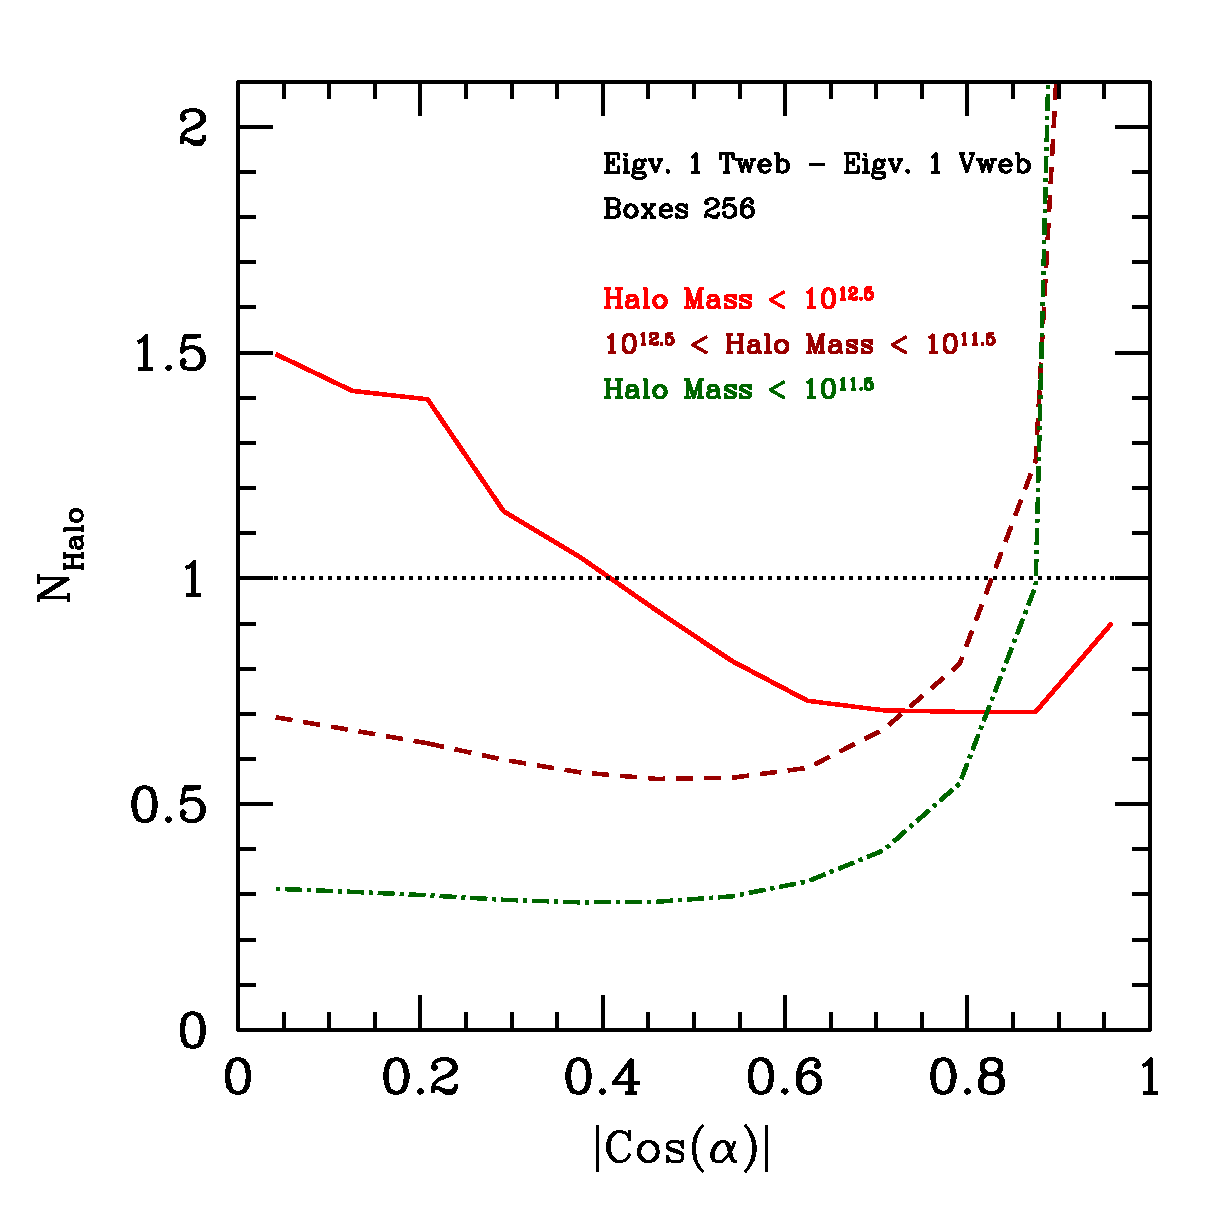
\includegraphics[width=0.30\textwidth]{../plot2/256/256_T1V1.ps}
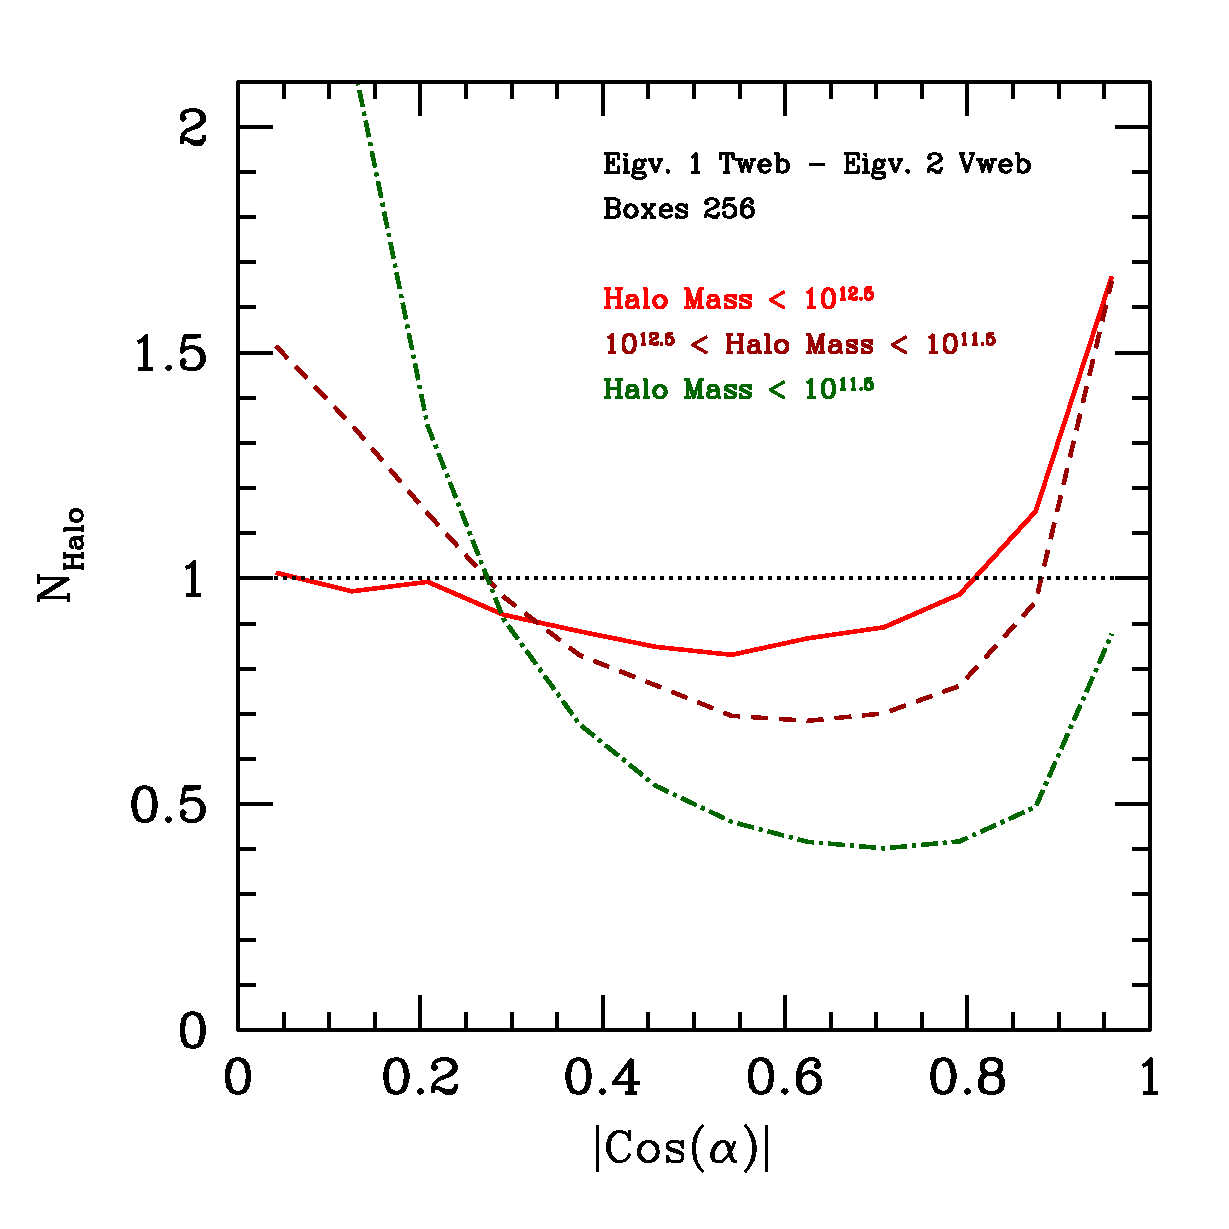
\includegraphics[width=0.30\textwidth]{../plot2/256/256_T1V2.ps}
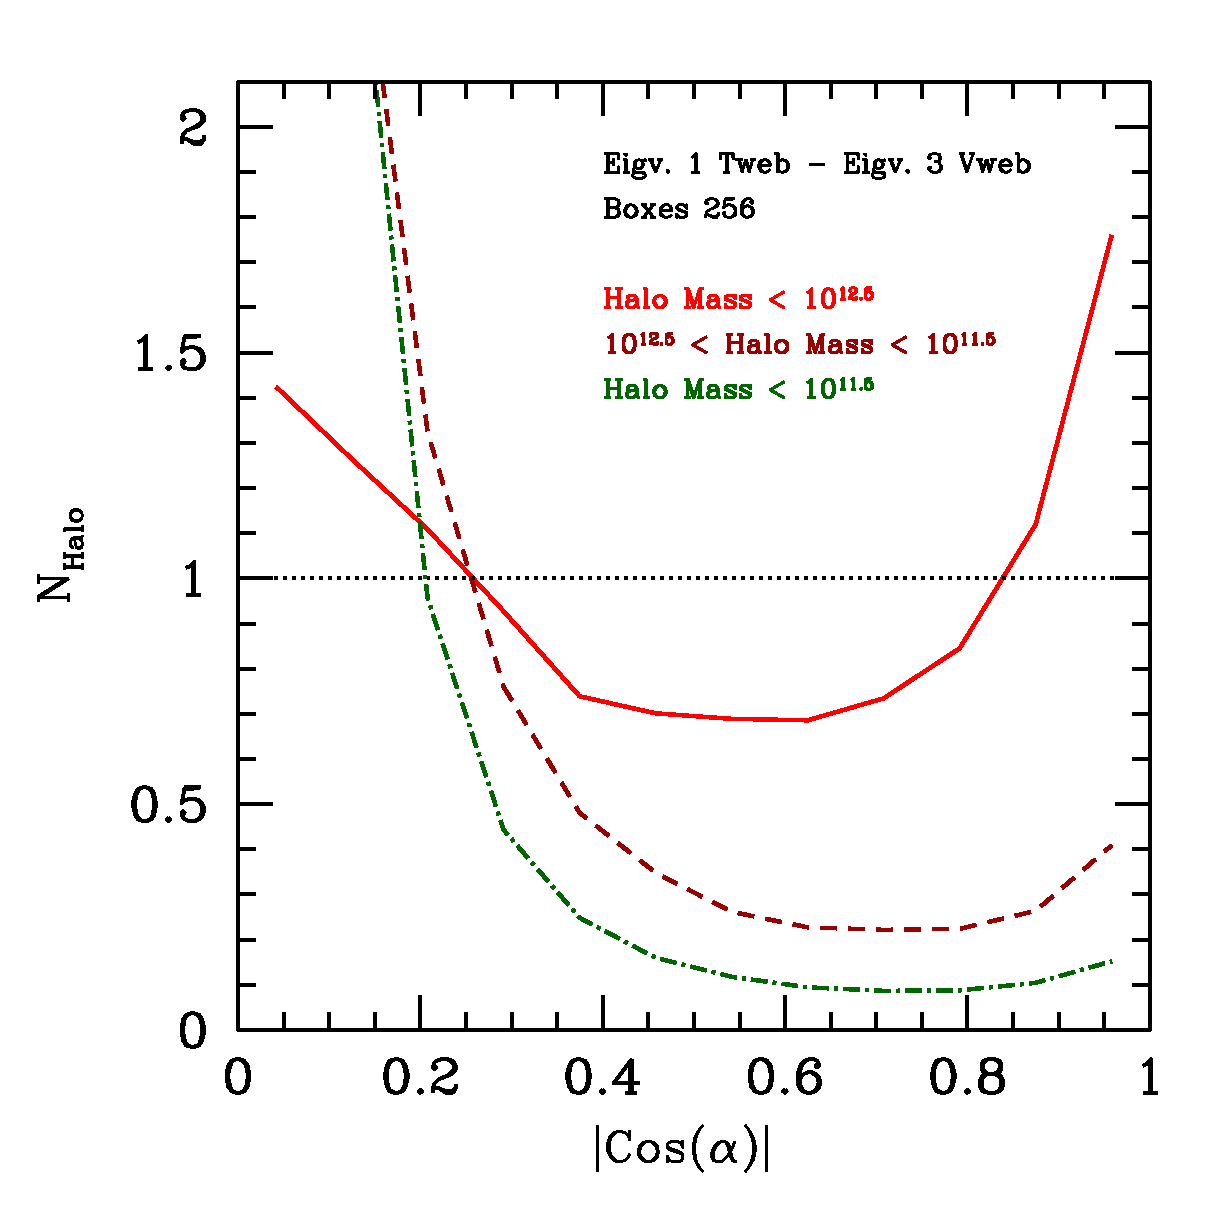
\includegraphics[width=0.30\textwidth]{../plot2/256/256_T1V3.ps}
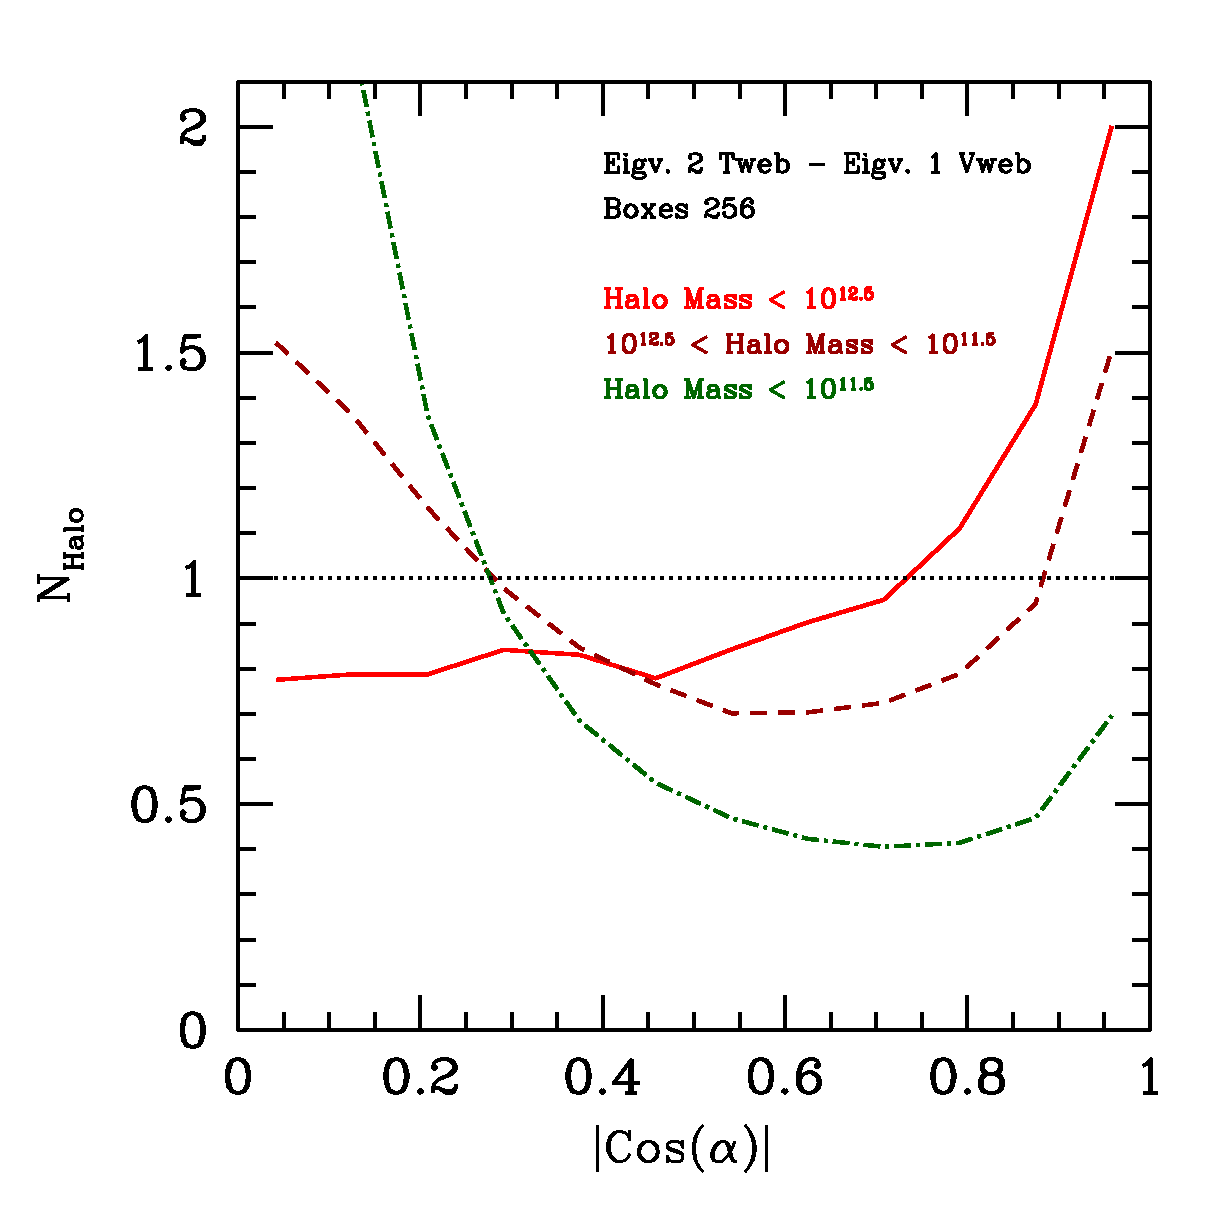
\includegraphics[width=0.30\textwidth]{../plot2/256/256_T2V1.ps}
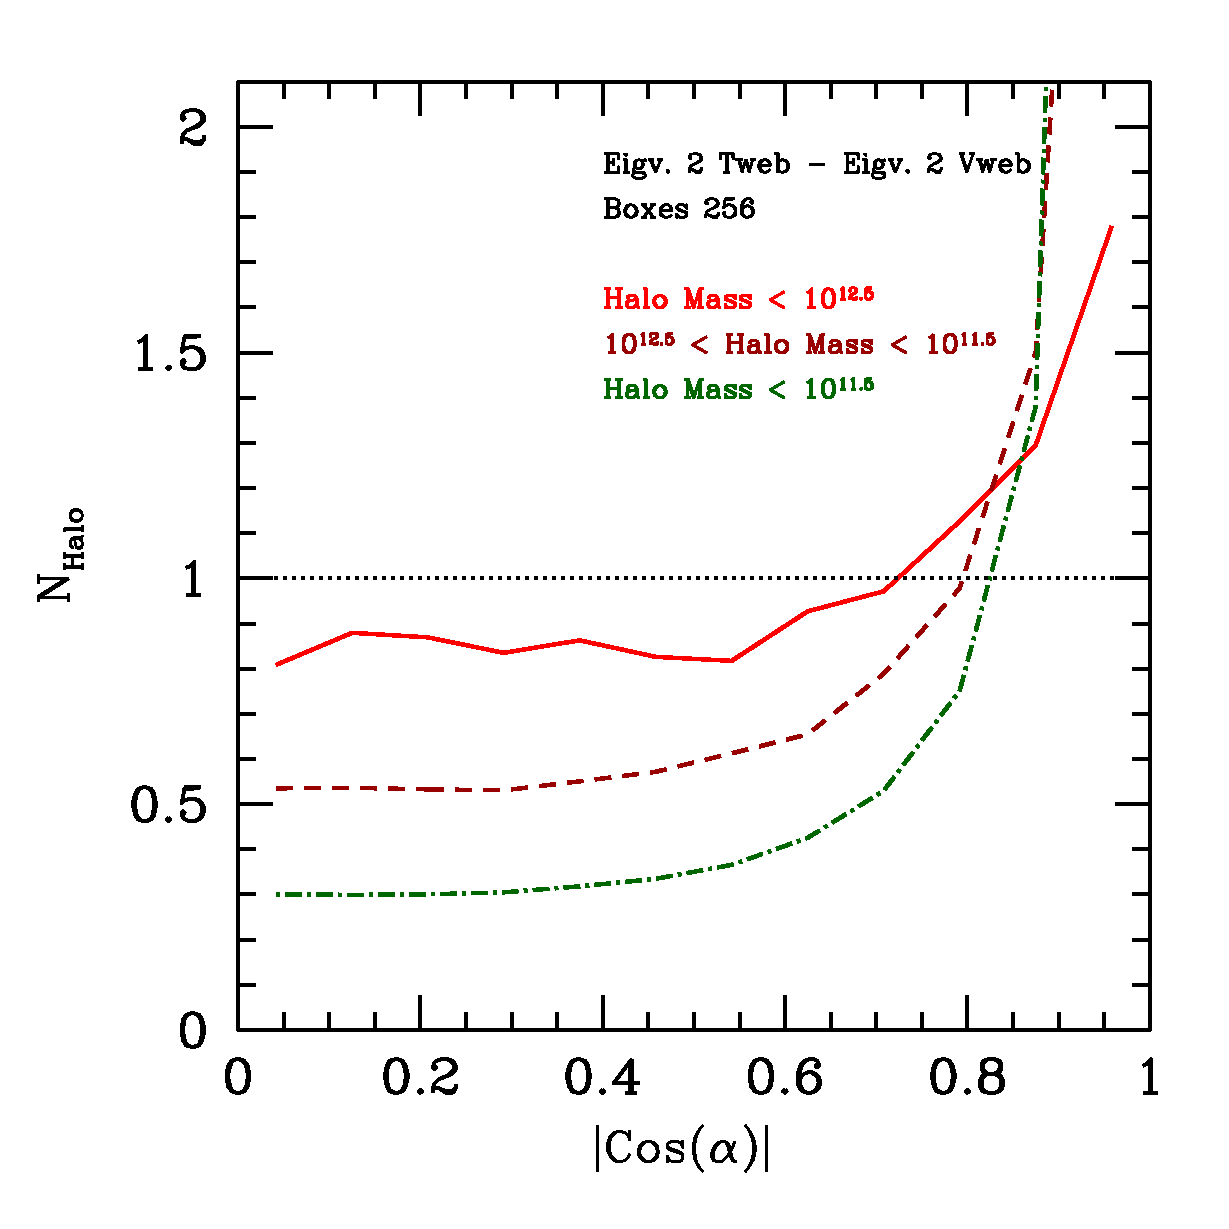
\includegraphics[width=0.30\textwidth]{../plot2/256/256_T2V2.ps}
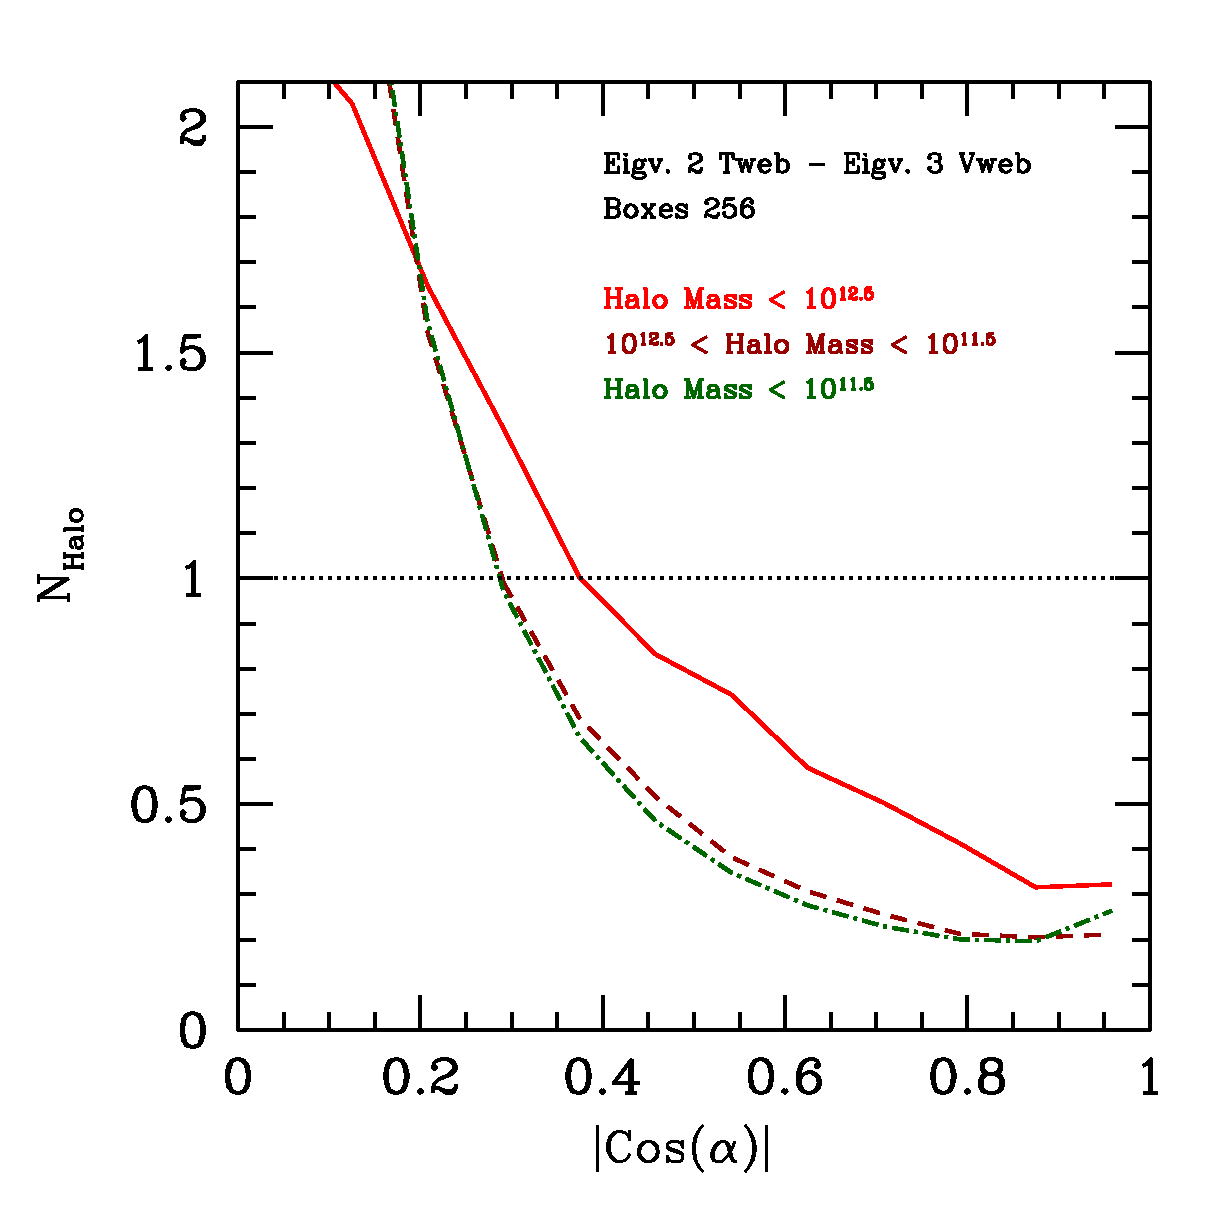
\includegraphics[width=0.30\textwidth]{../plot2/256/256_T2V3.ps}
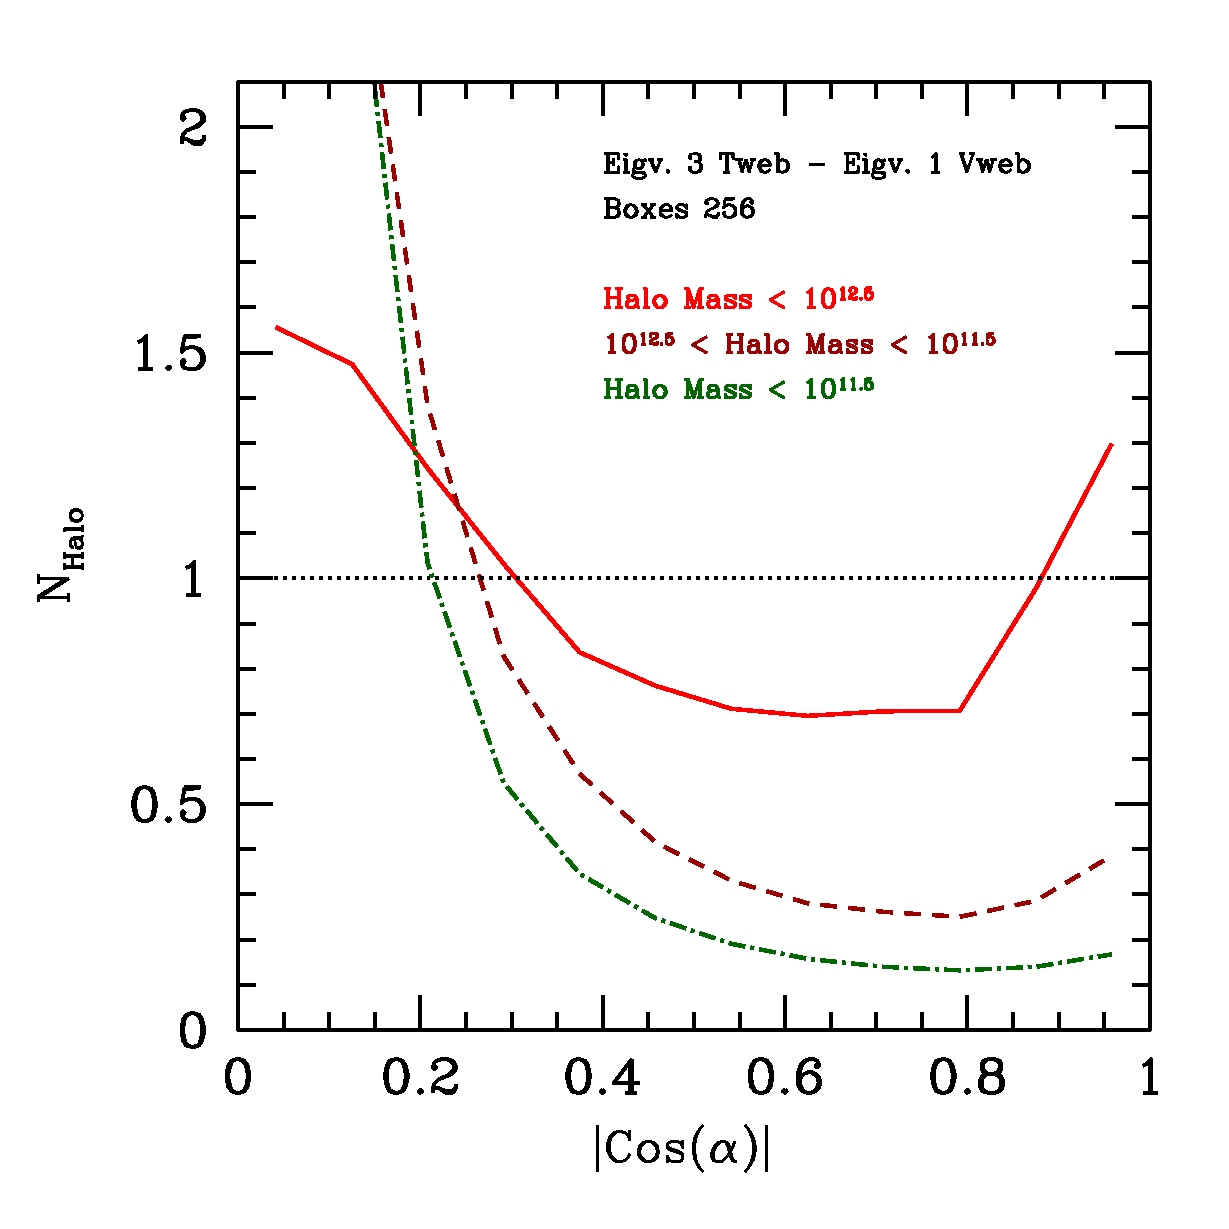
\includegraphics[width=0.30\textwidth]{../plot2/256/256_T3V1.ps}
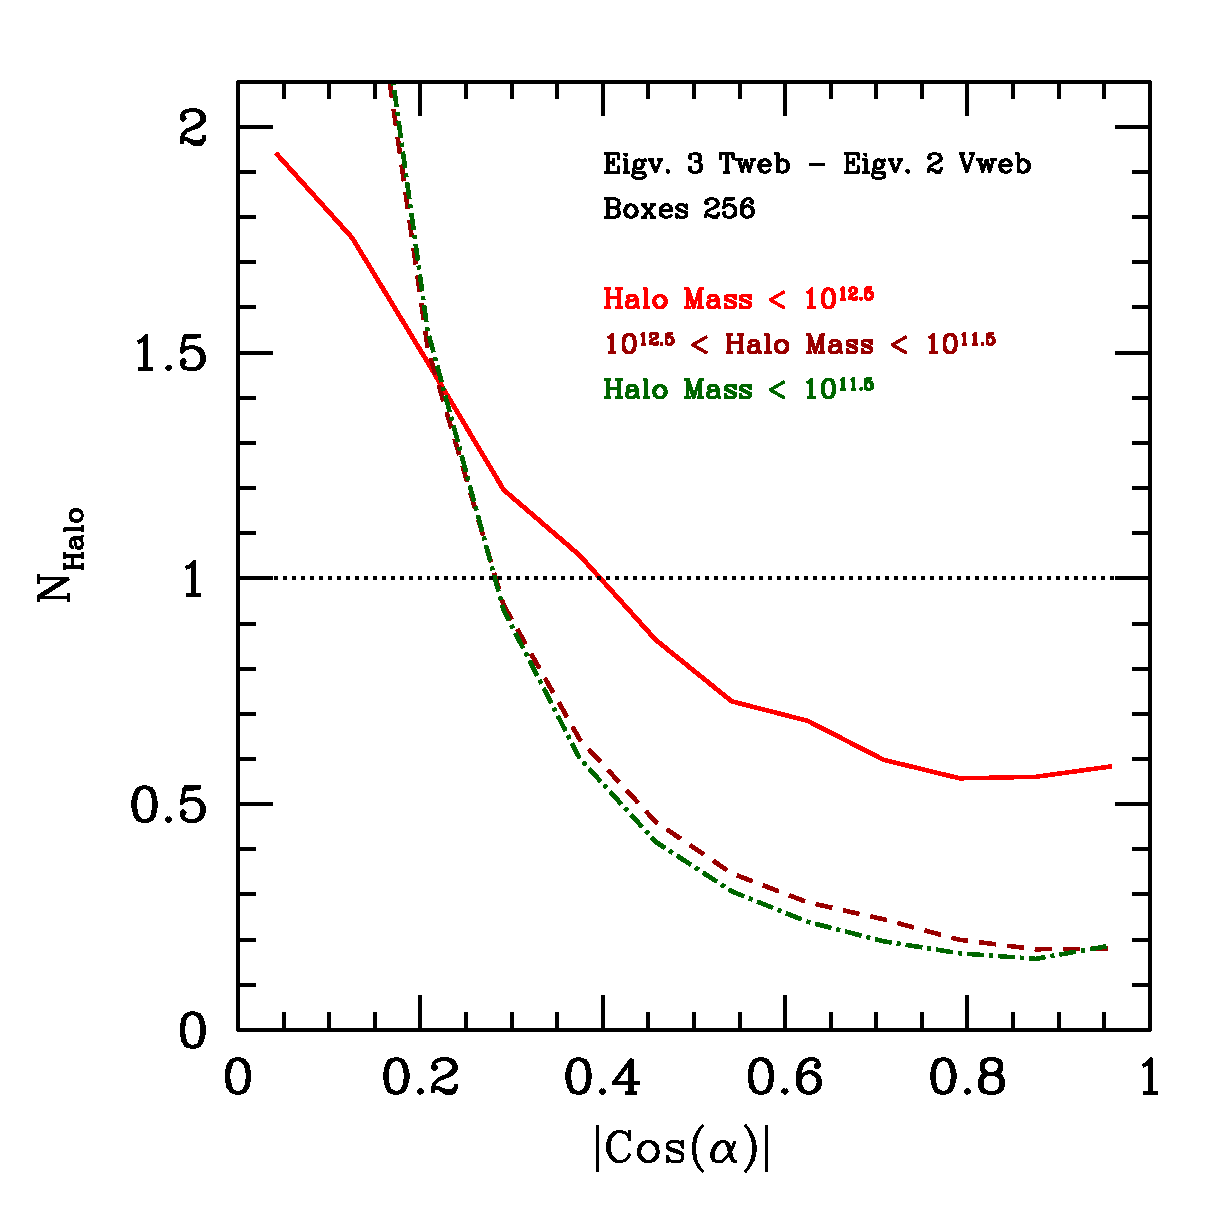
\includegraphics[width=0.30\textwidth]{../plot2/256/256_T3V2.ps}
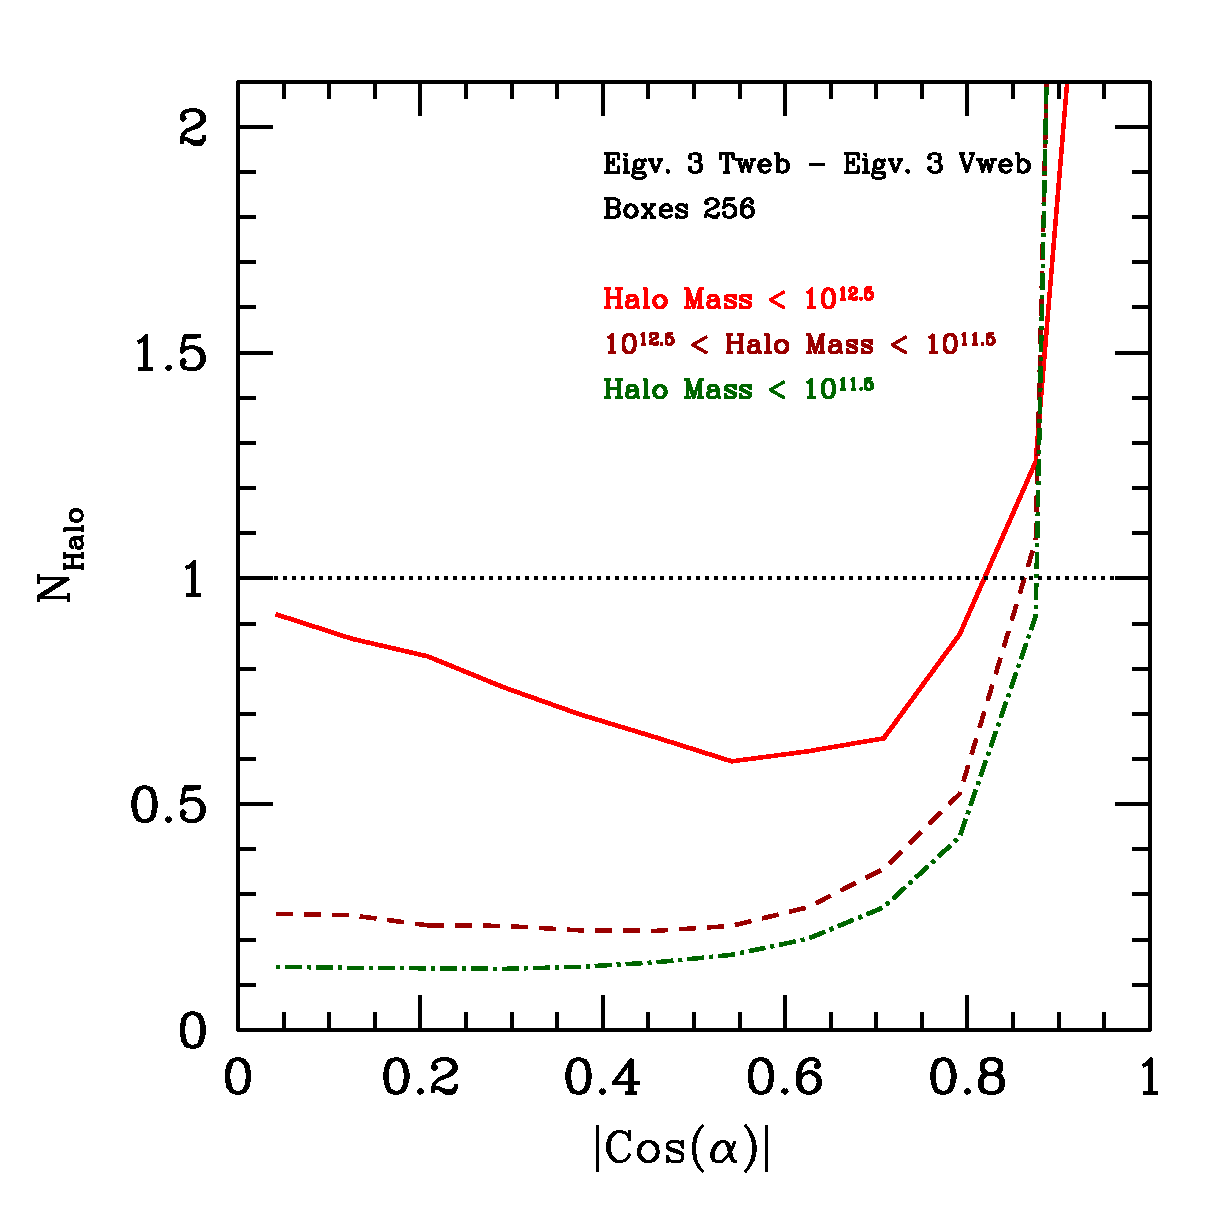
\includegraphics[width=0.30\textwidth]{../plot2/256/256_T3V3.ps}
\caption{Interweb alignment for $256^3$ grid resolution.}
\end{figure*}

\begin{figure*}
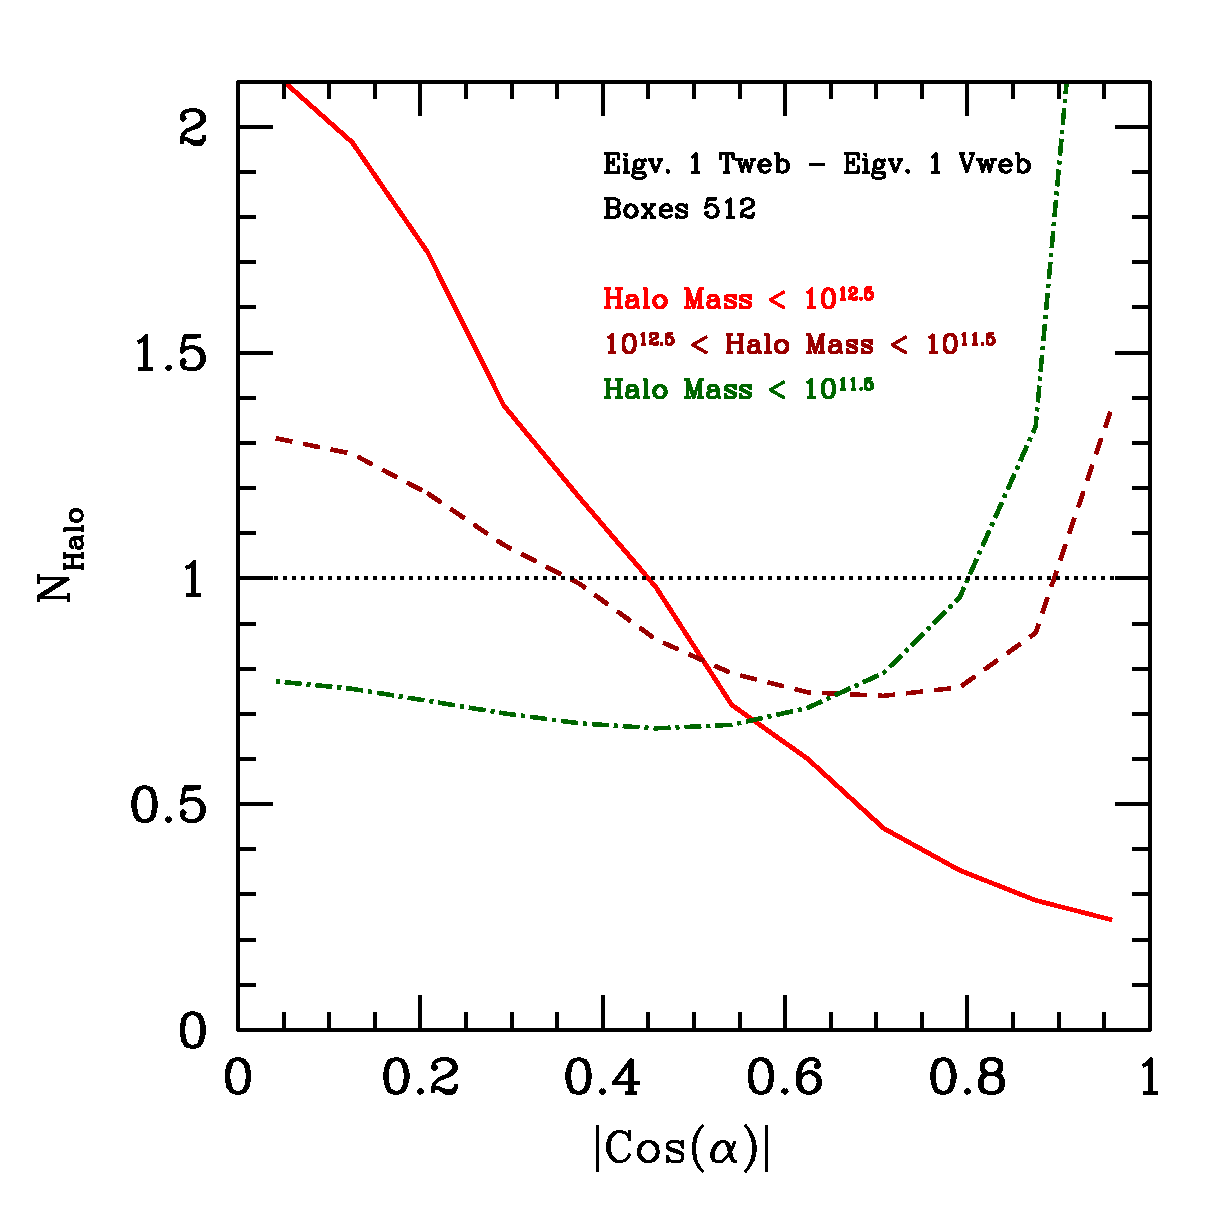
\includegraphics[width=0.30\textwidth]{../plot2/512/512_T1V1.ps}
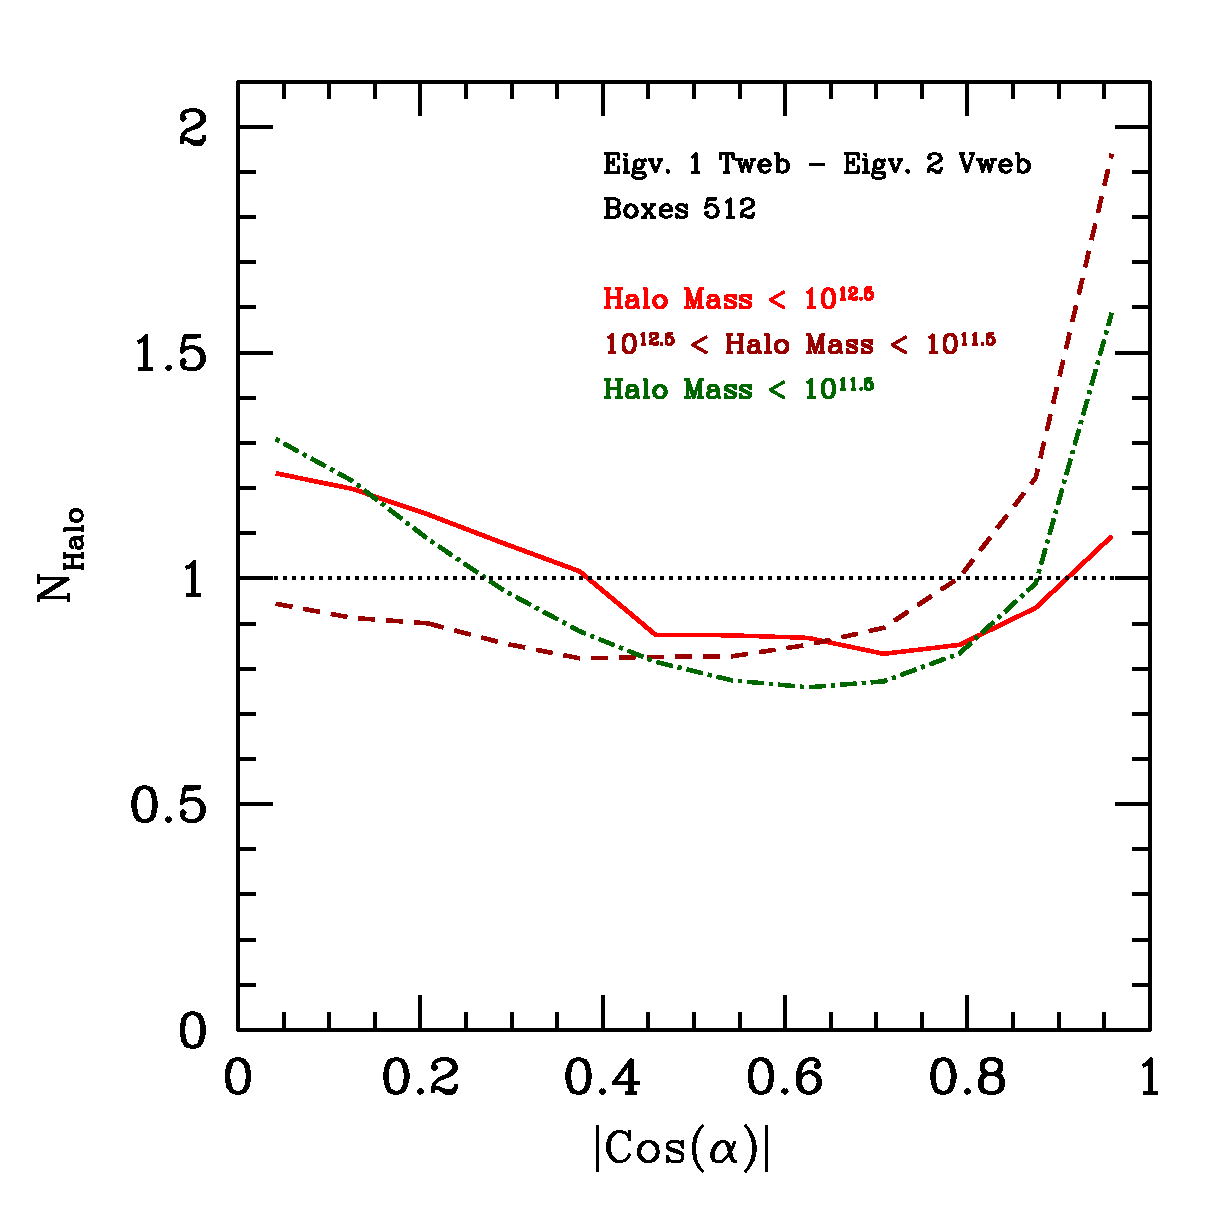
\includegraphics[width=0.30\textwidth]{../plot2/512/512_T1V2.ps}
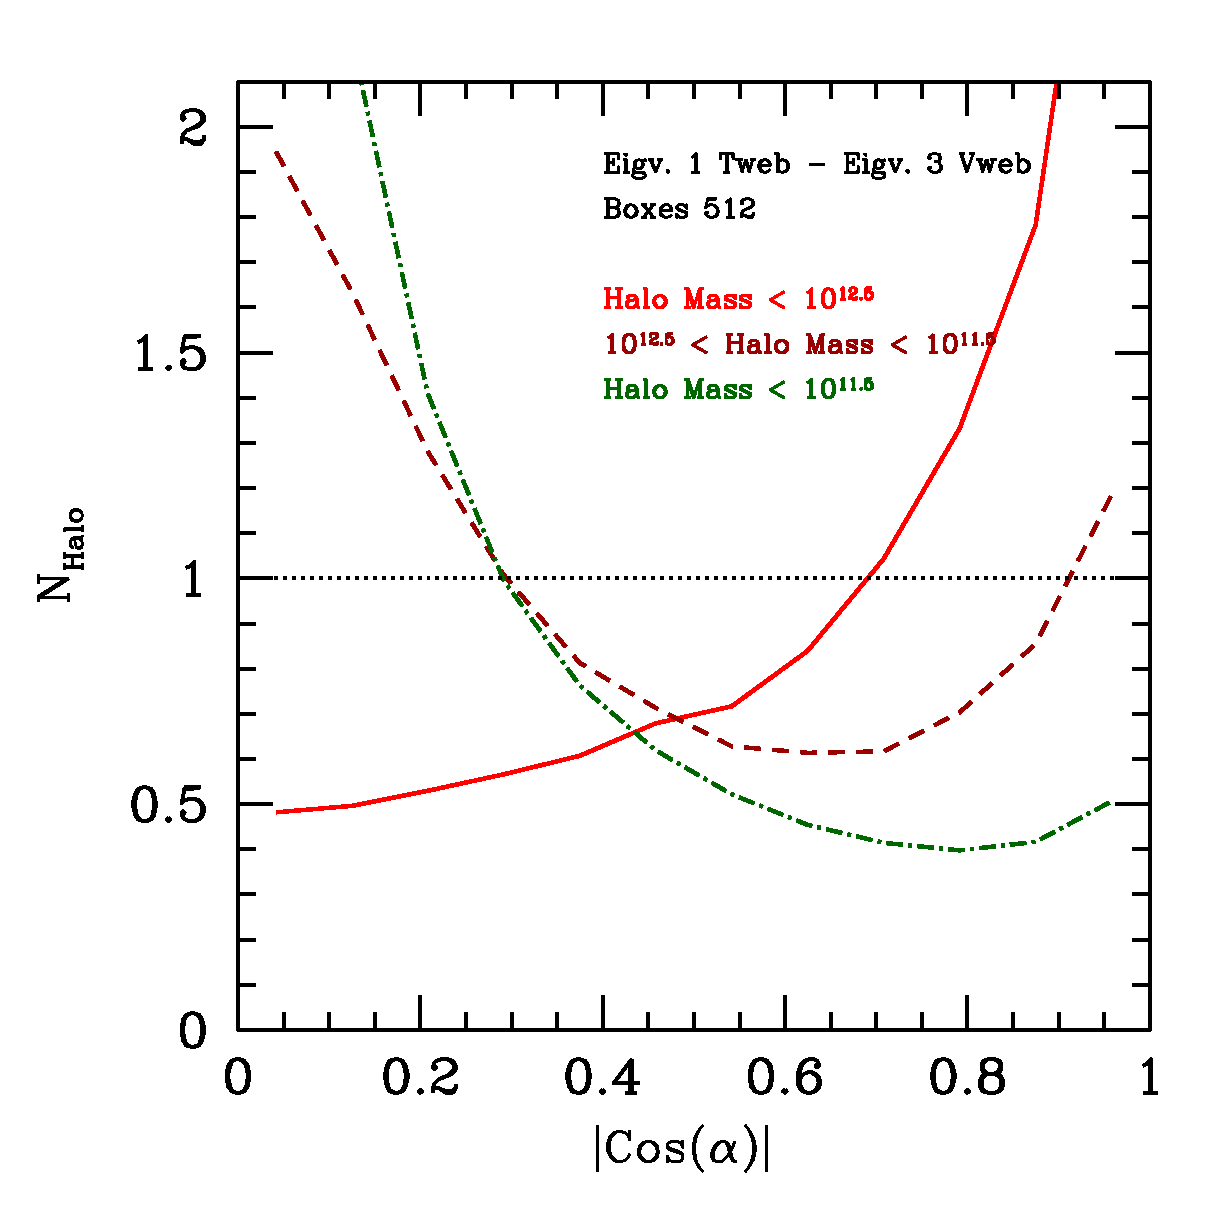
\includegraphics[width=0.30\textwidth]{../plot2/512/512_T1V3.ps}
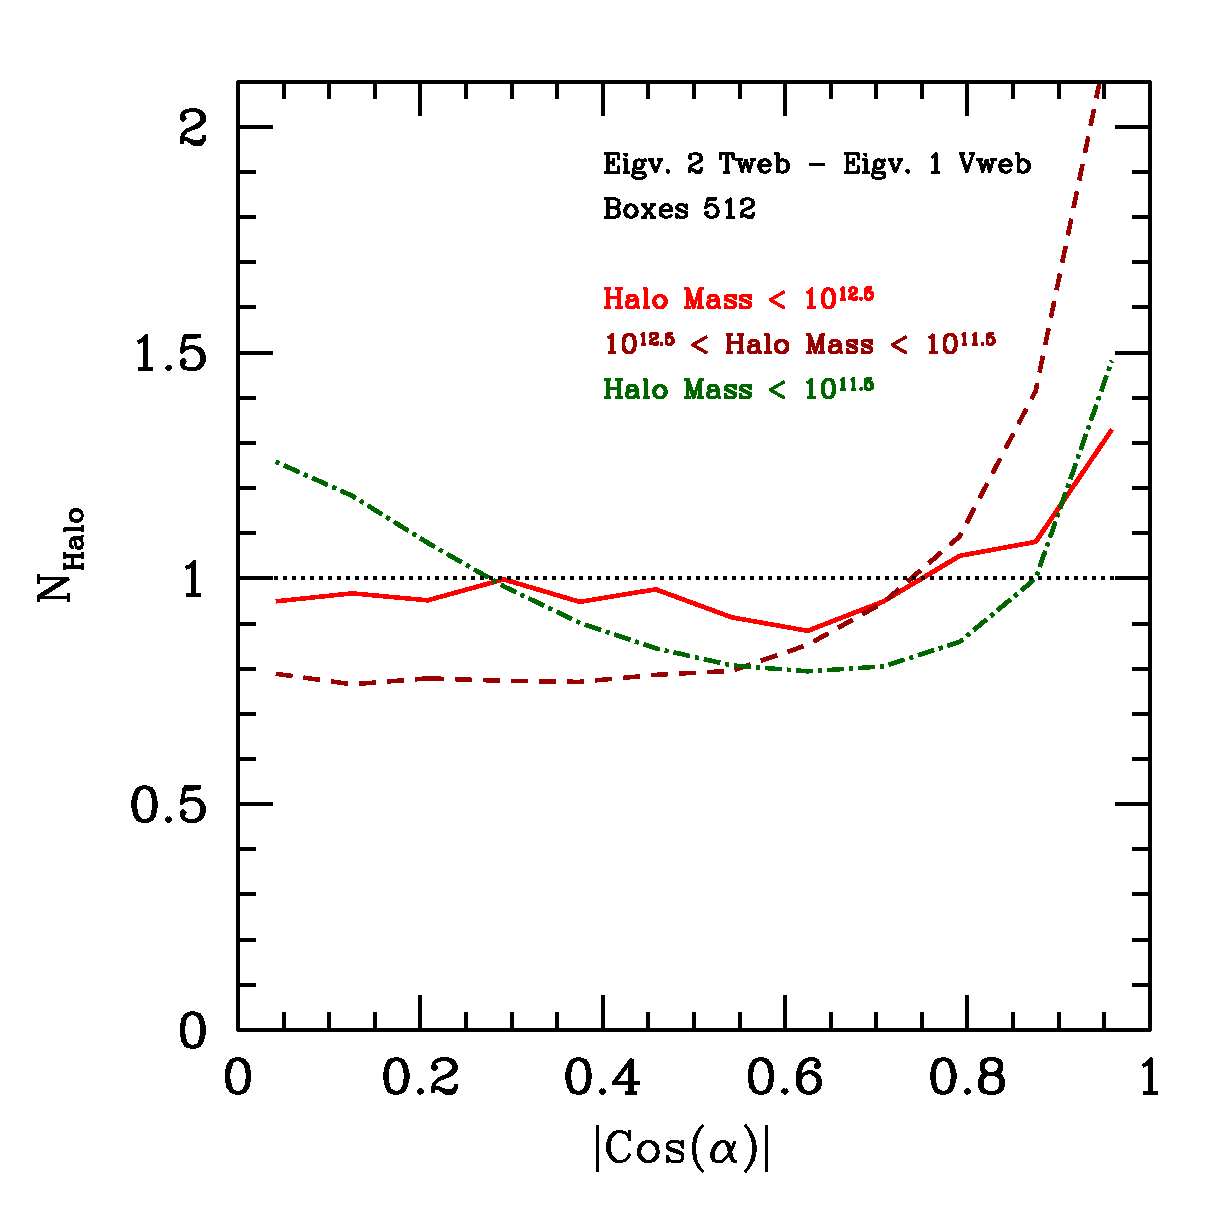
\includegraphics[width=0.30\textwidth]{../plot2/512/512_T2V1.ps}
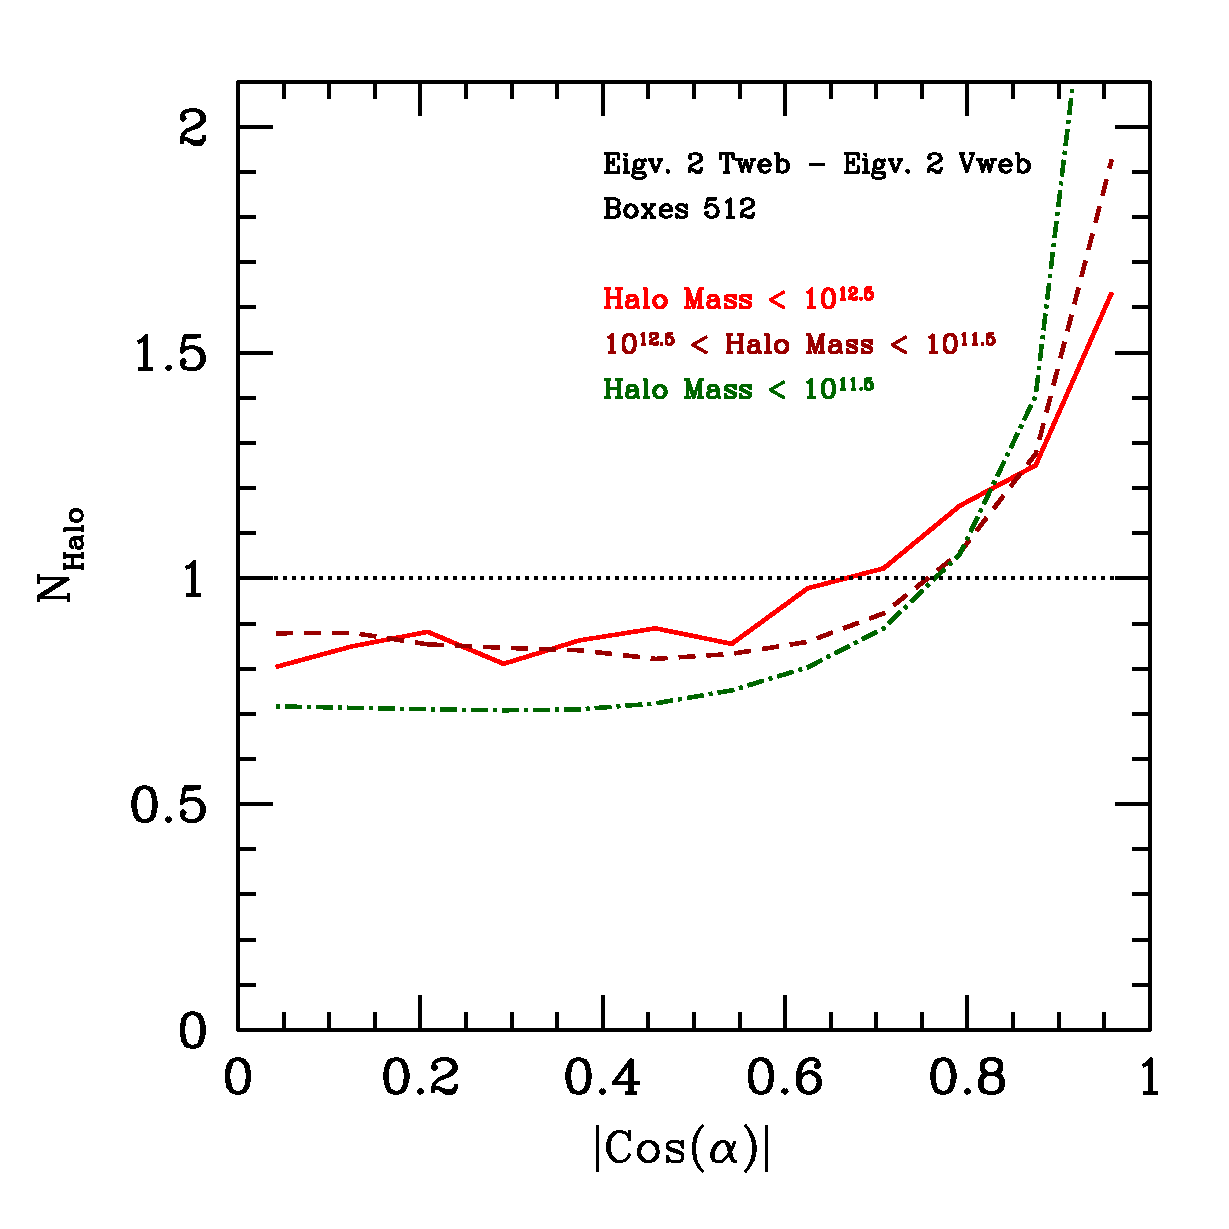
\includegraphics[width=0.30\textwidth]{../plot2/512/512_T2V2.ps}
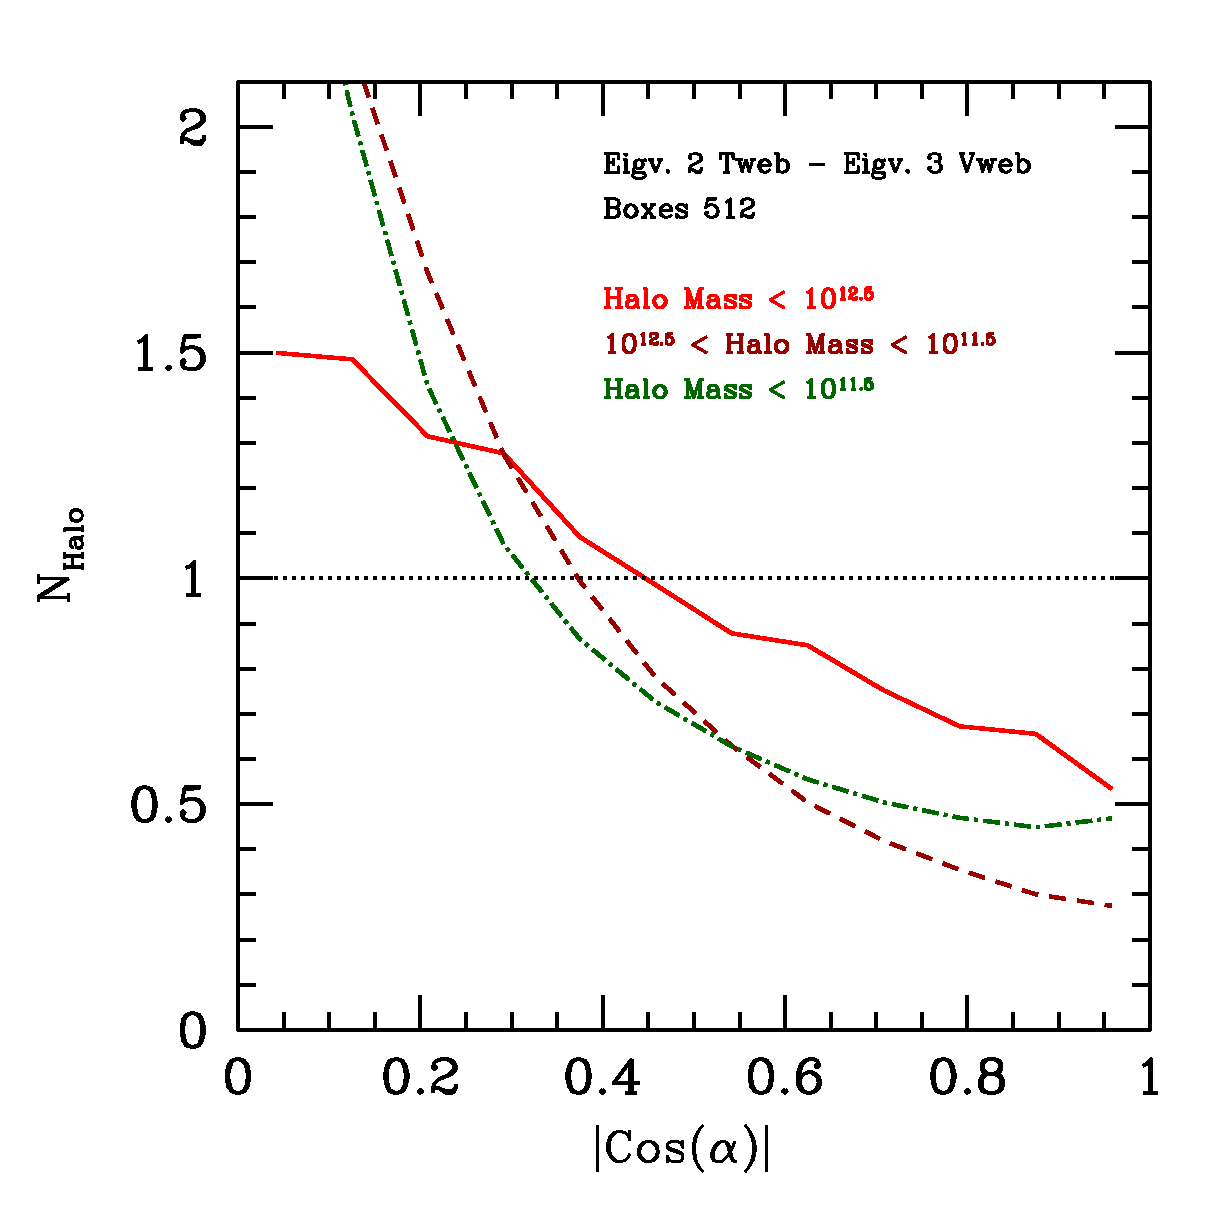
\includegraphics[width=0.30\textwidth]{../plot2/512/512_T2V3.ps}
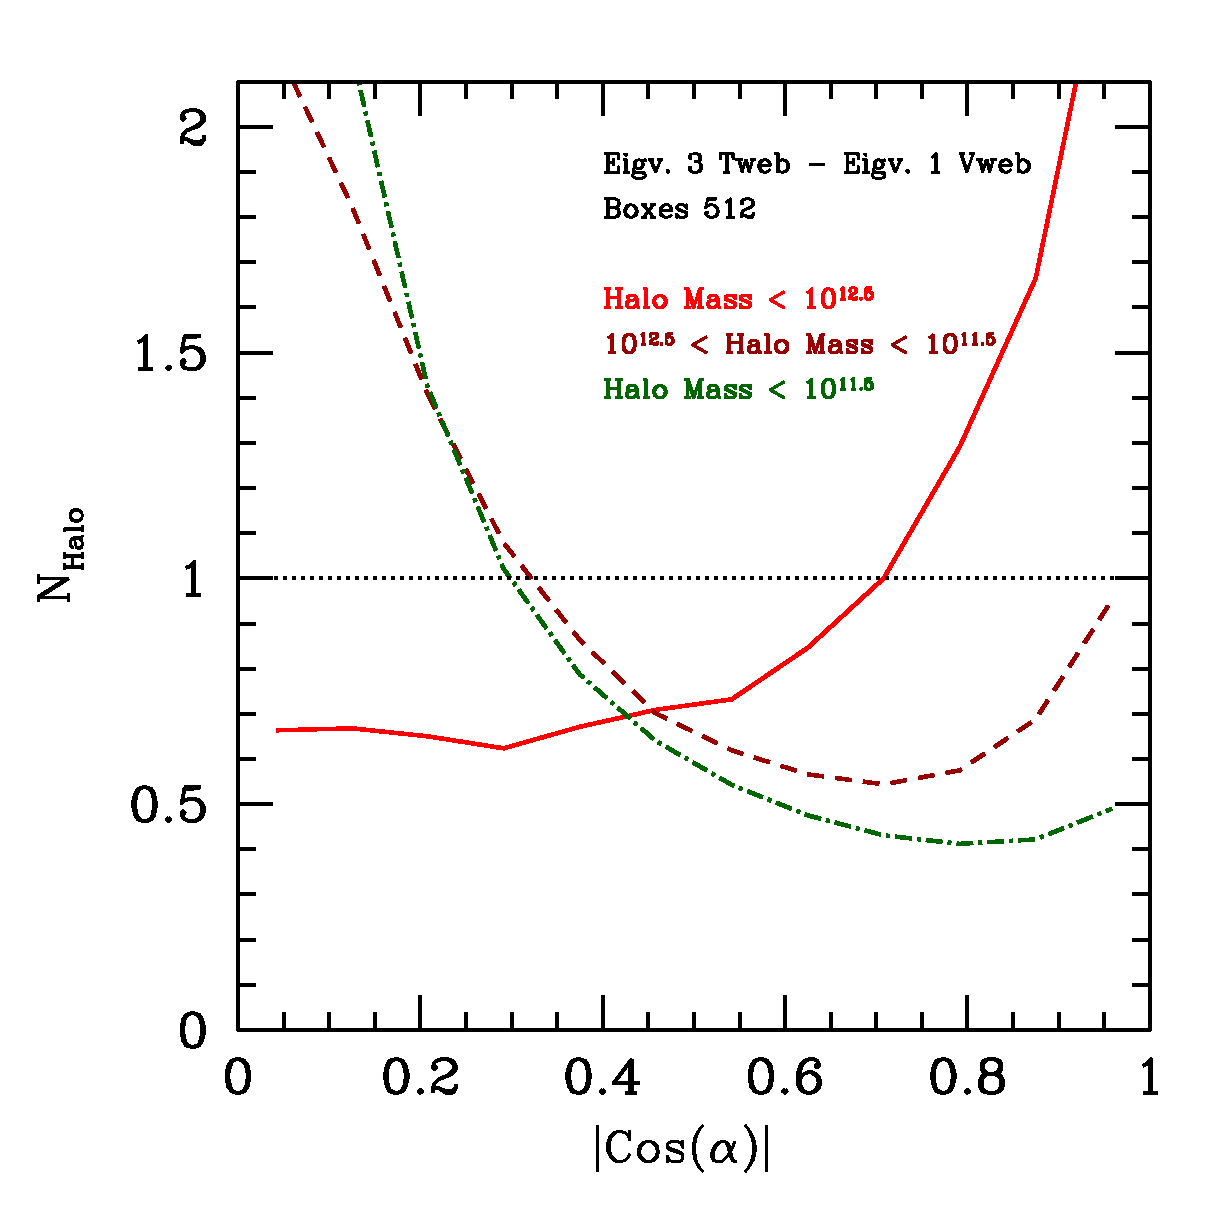
\includegraphics[width=0.30\textwidth]{../plot2/512/512_T3V1.ps}
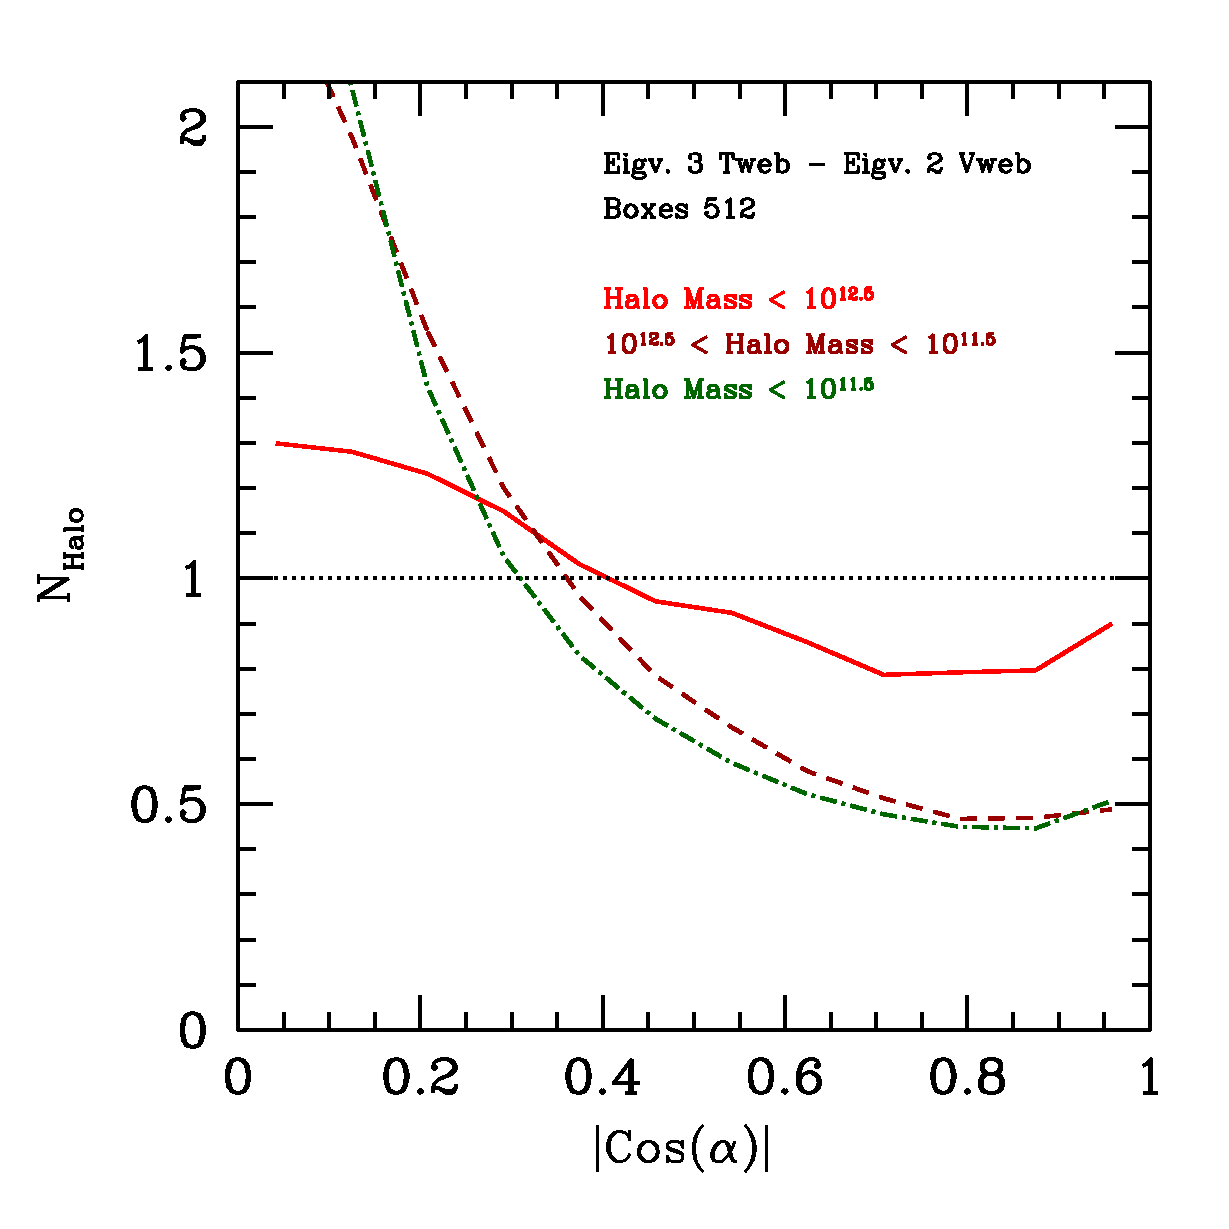
\includegraphics[width=0.30\textwidth]{../plot2/512/512_T3V2.ps}
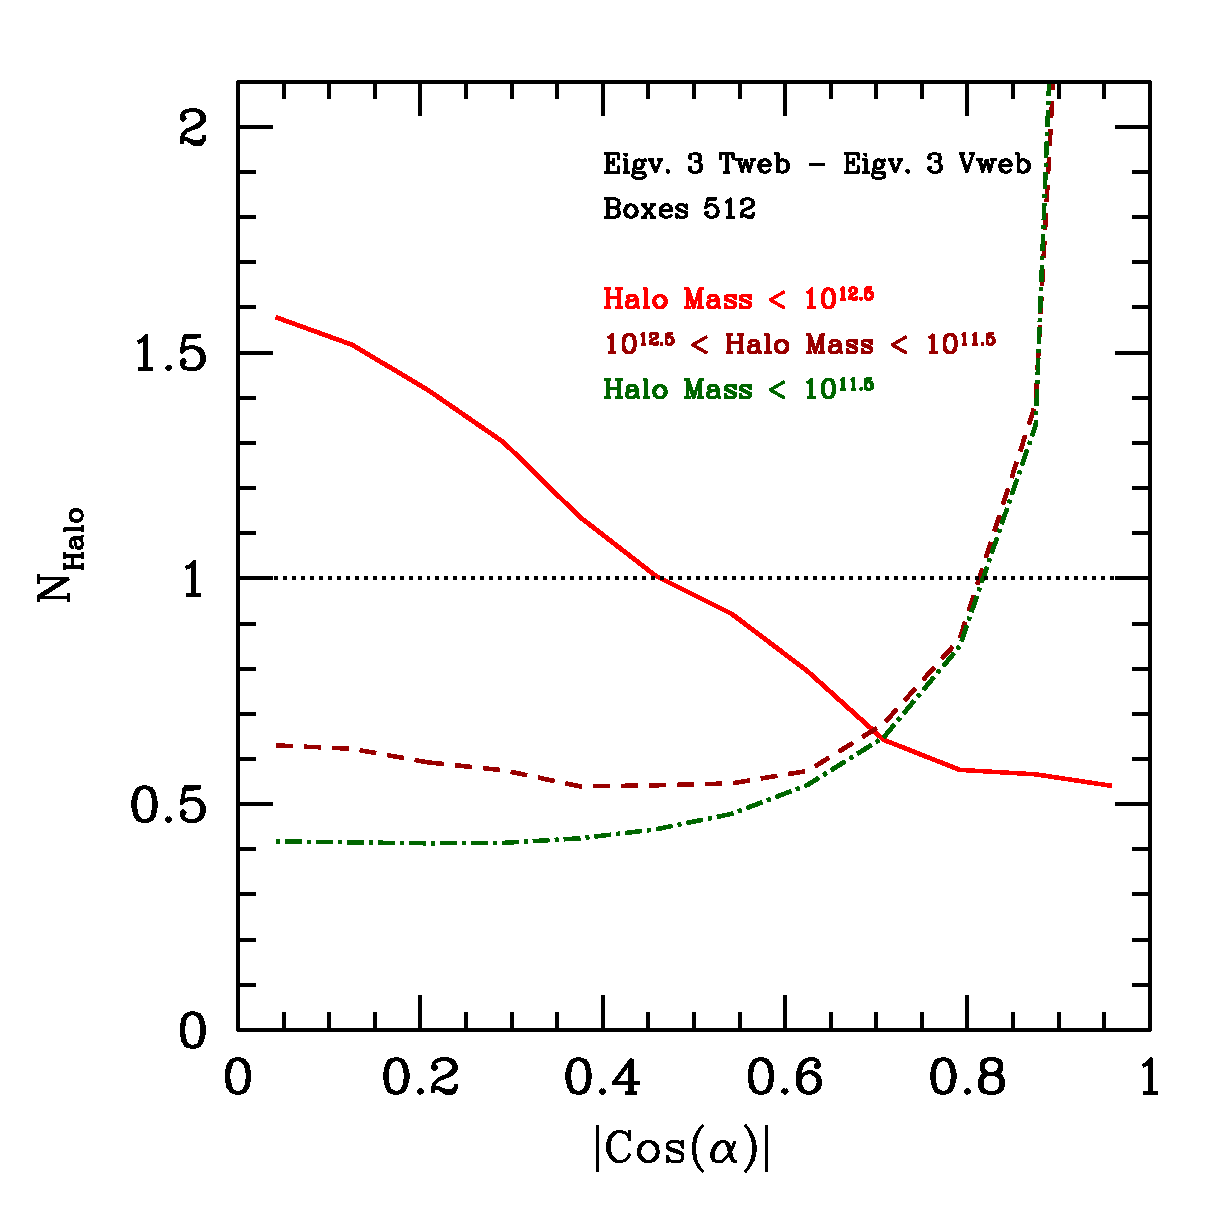
\includegraphics[width=0.30\textwidth]{../plot2/512/512_T3V3.ps}
\caption{Interweb alignment for $512^3$ grid resolution.}
\end{figure*}



\subsection{Shape Alignment}

\begin{figure*}
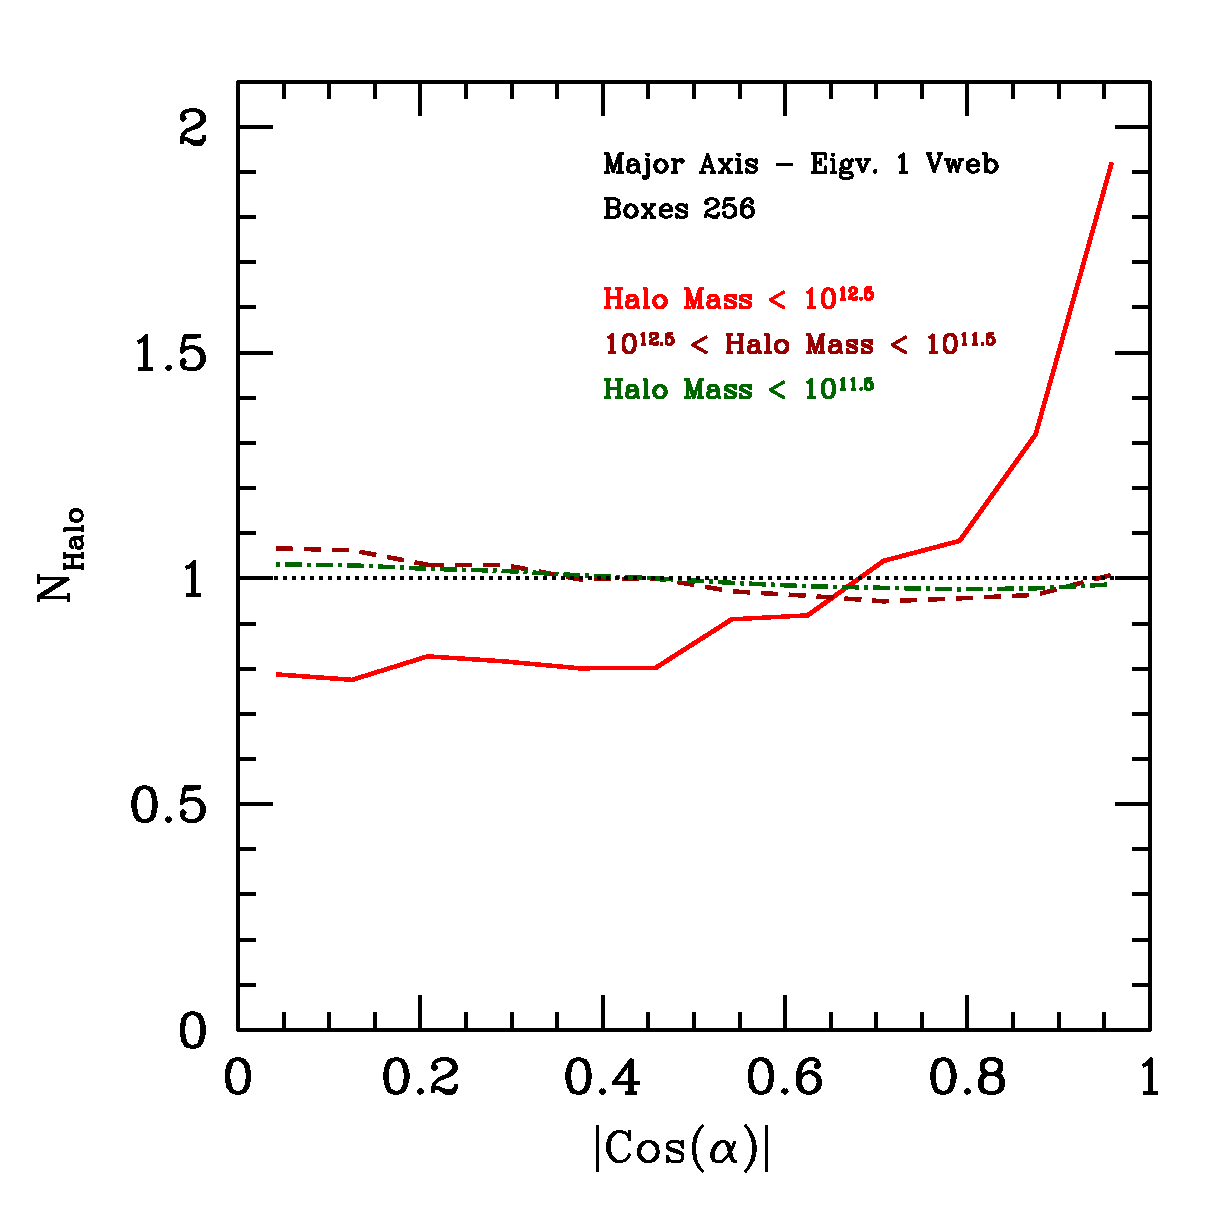
\includegraphics[width=0.30\textwidth]{../plot2/Ax1_VT/256_AX1_V1.ps}
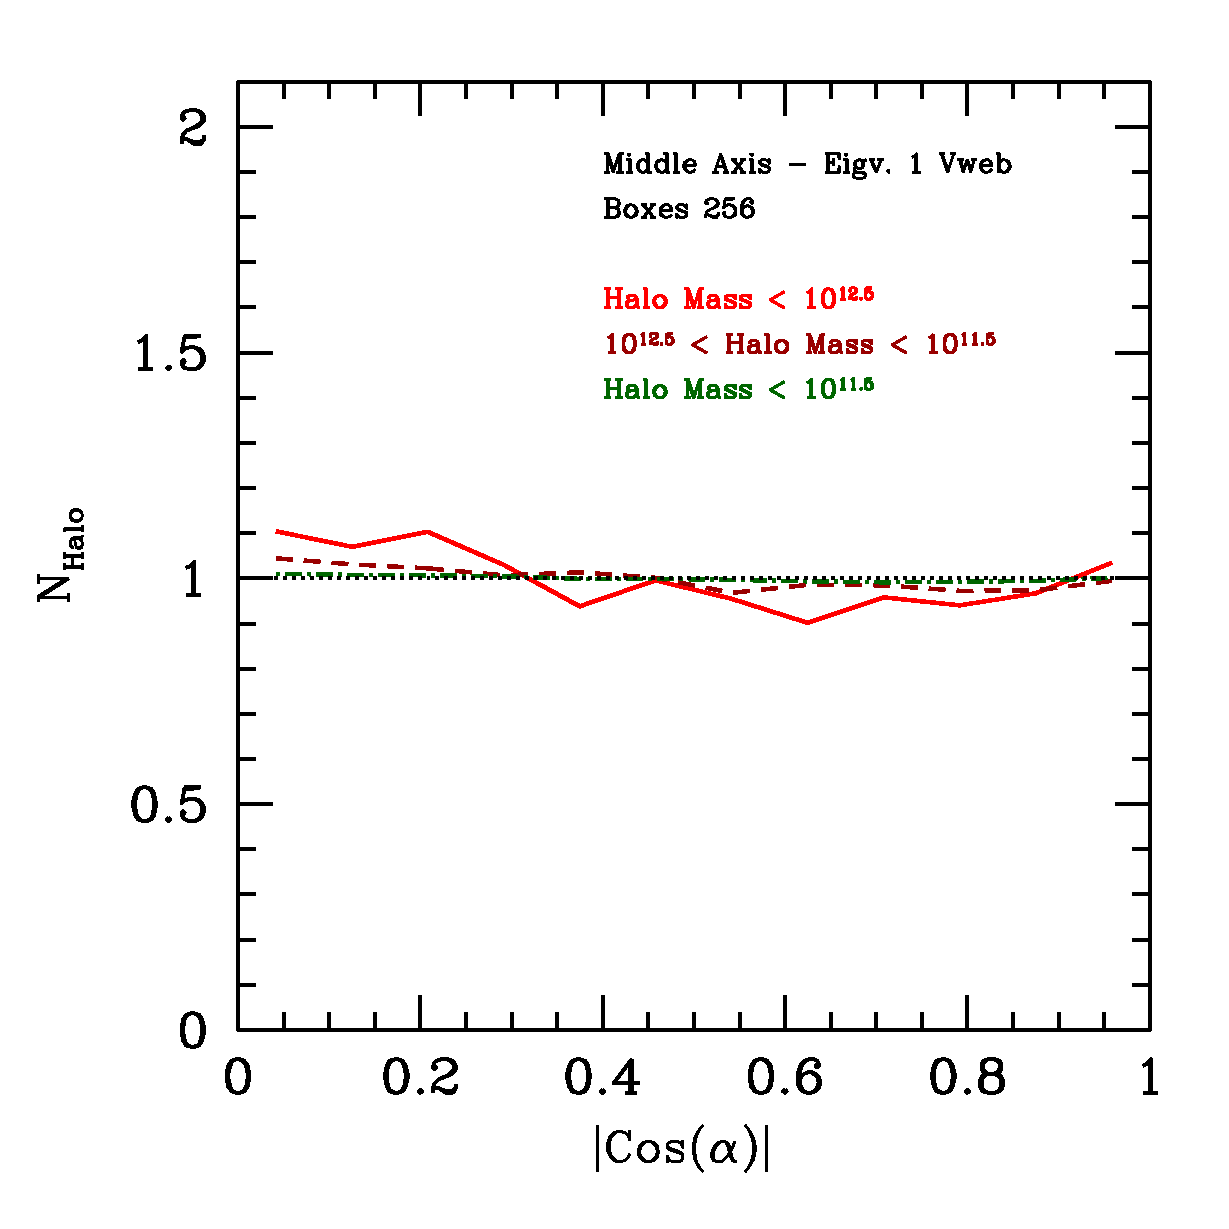
\includegraphics[width=0.30\textwidth]{../plot2/Ax2_VT/256_AX2_V1.ps}
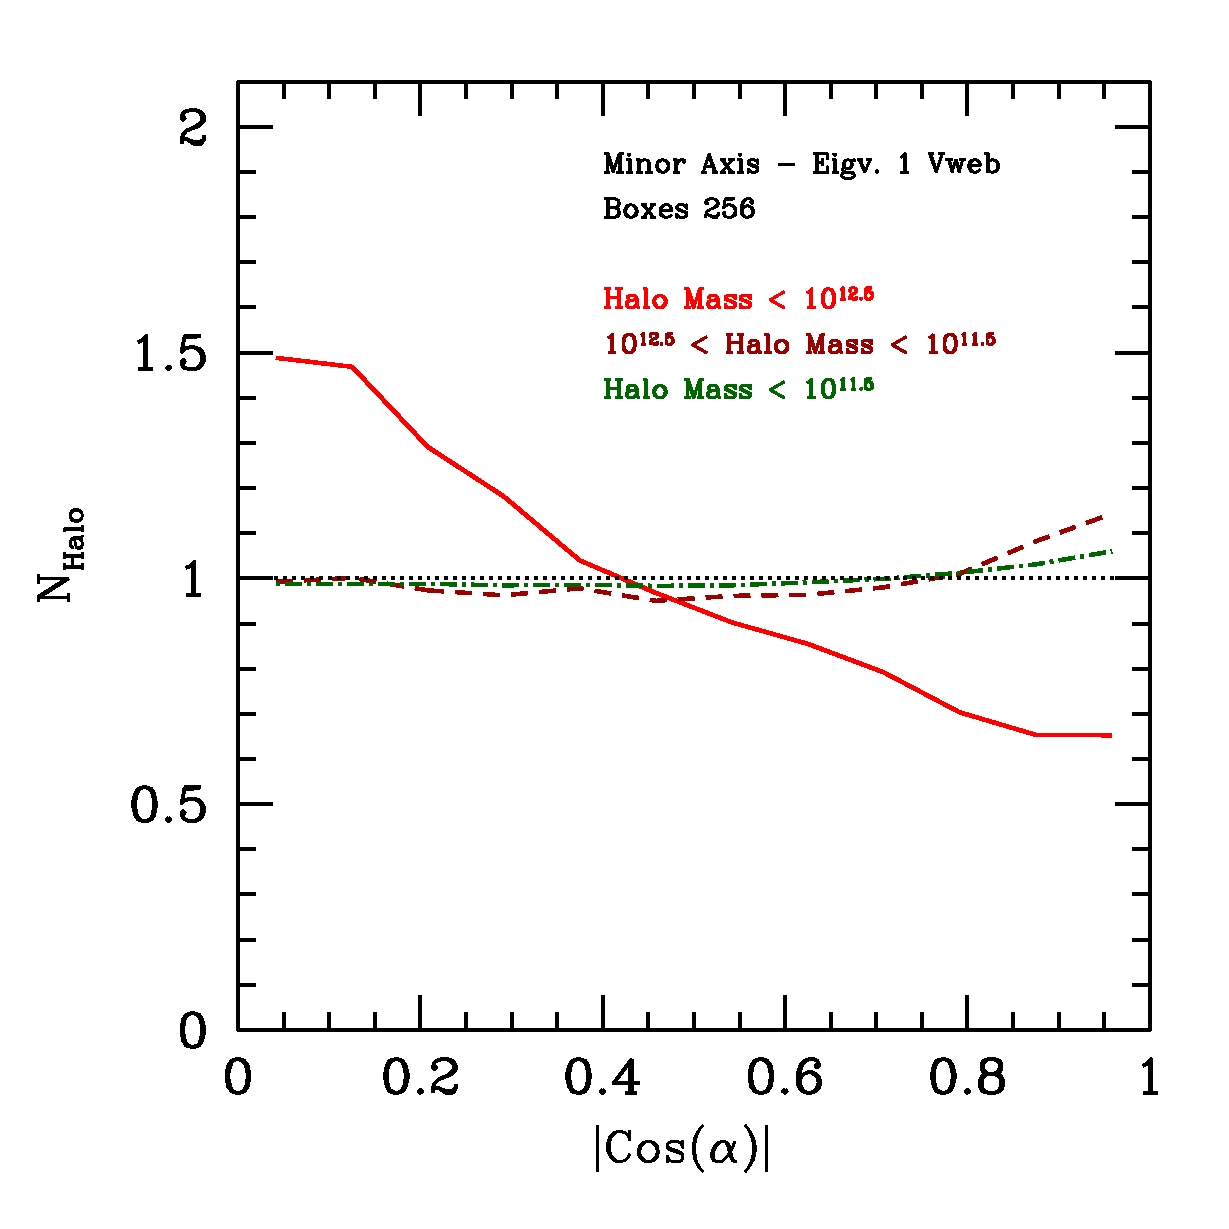
\includegraphics[width=0.30\textwidth]{../plot2/Ax3_VT/256_AX3_V1.ps}
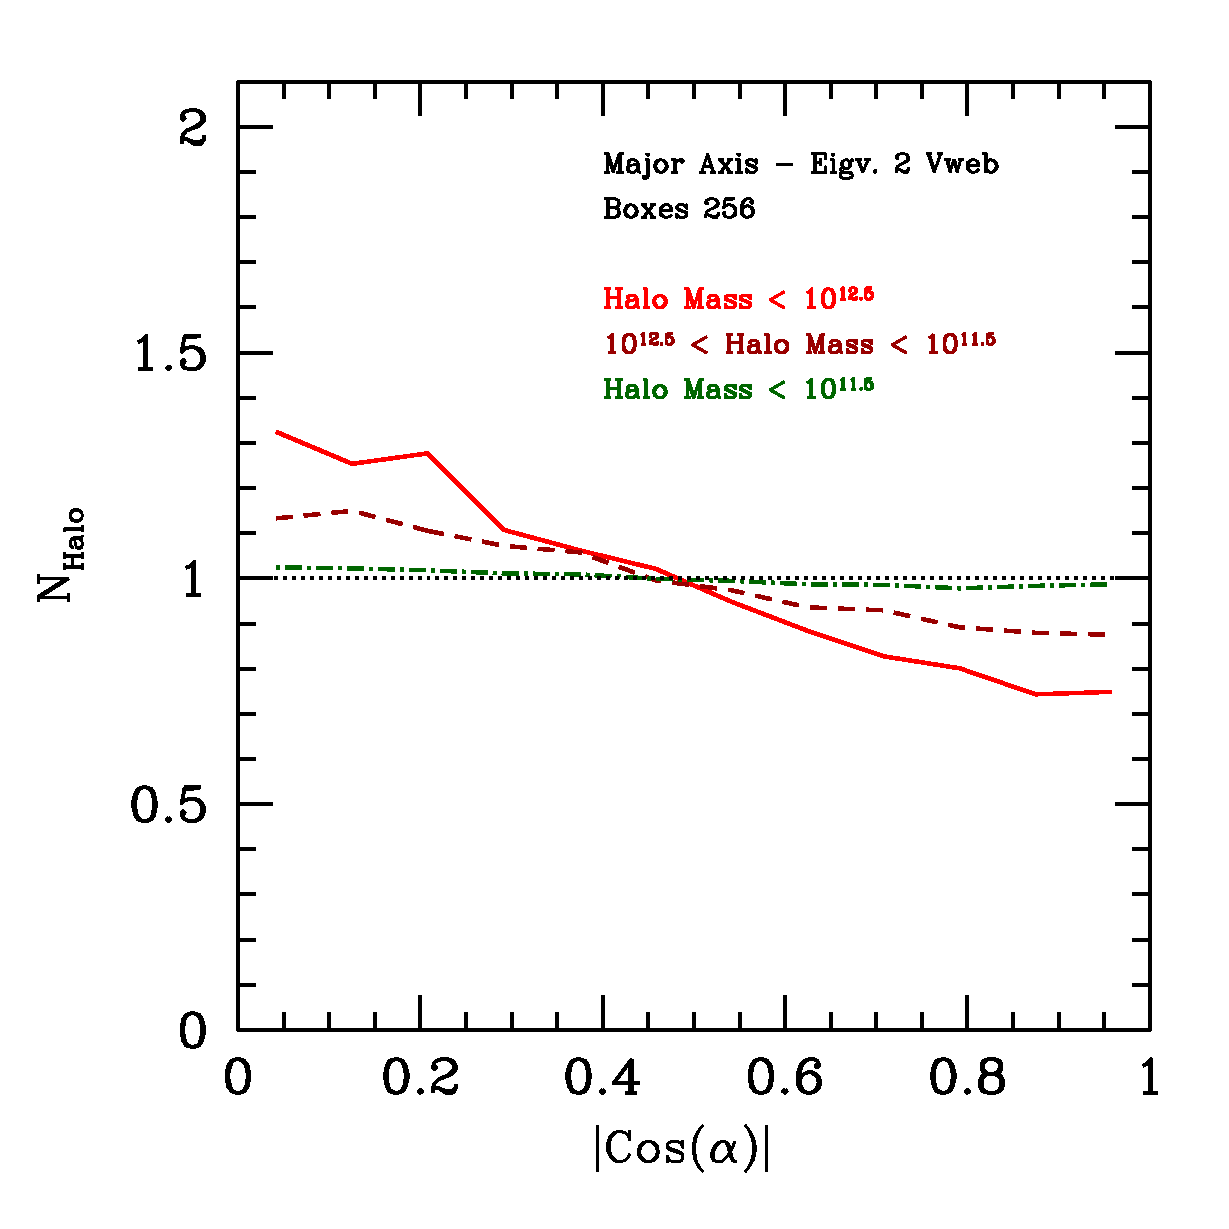
\includegraphics[width=0.30\textwidth]{../plot2/Ax1_VT/256_AX1_V2.ps}
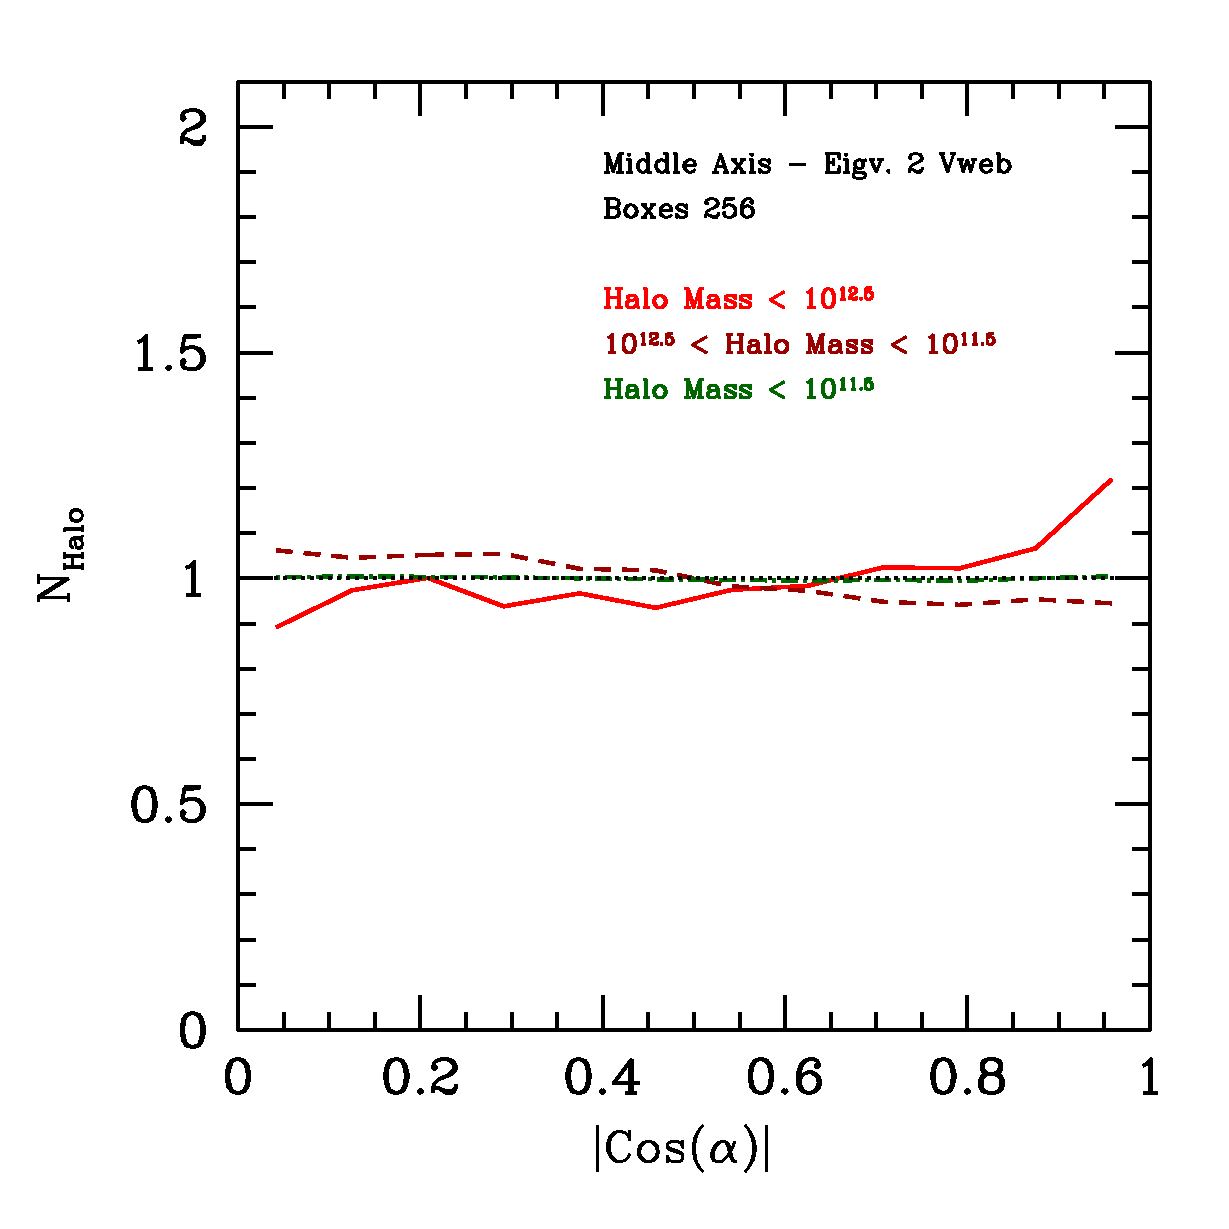
\includegraphics[width=0.30\textwidth]{../plot2/Ax2_VT/256_AX2_V2.ps}
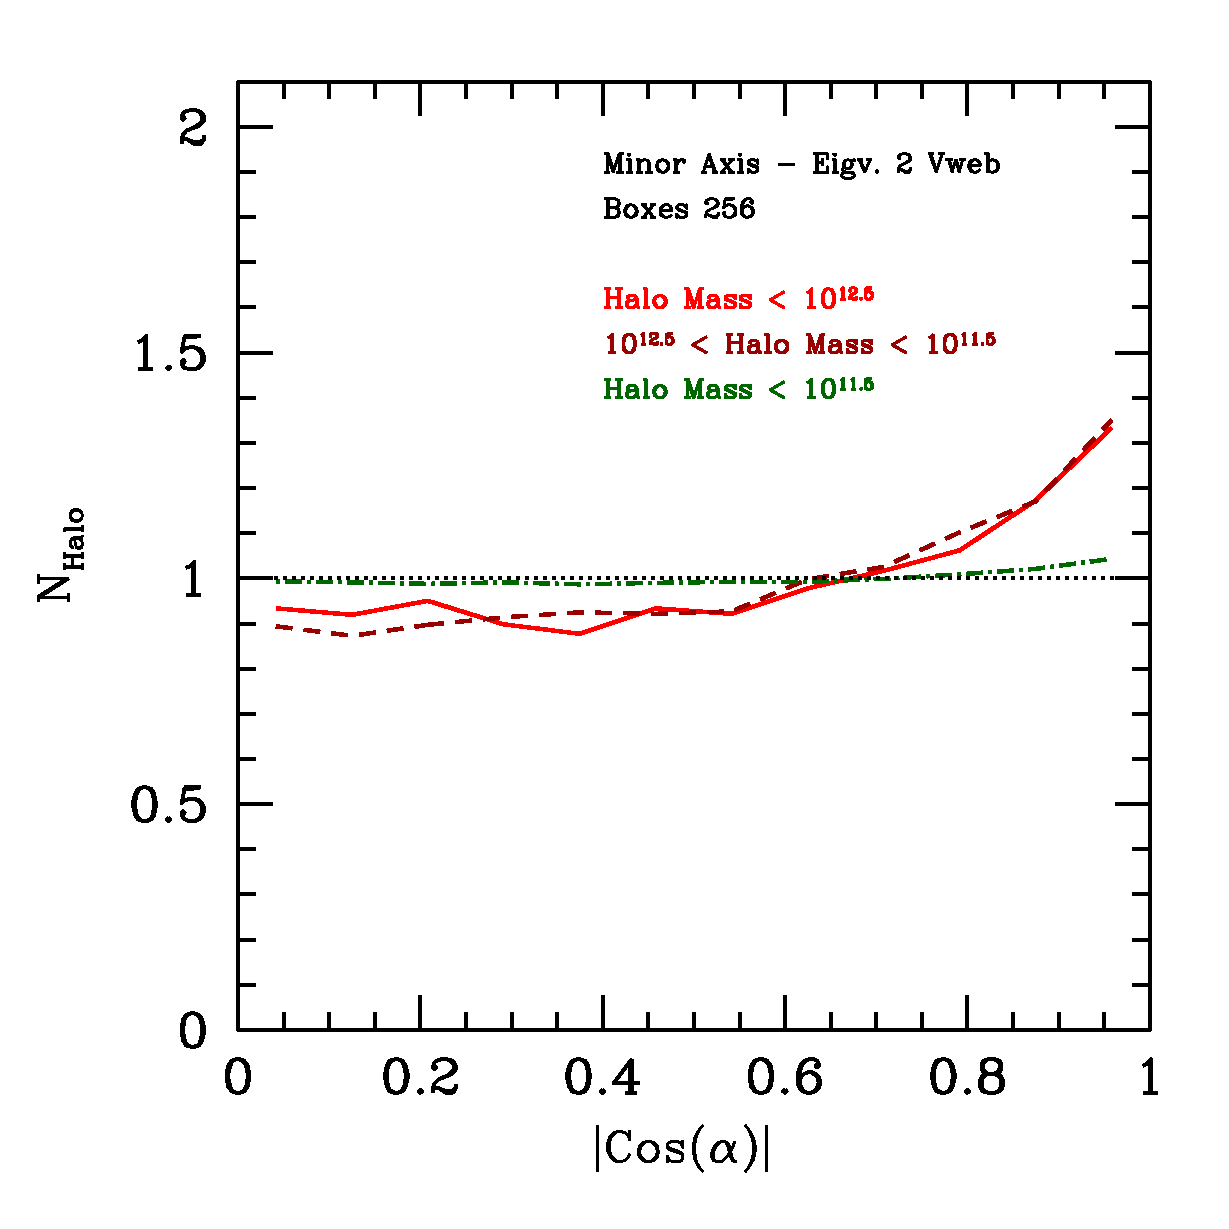
\includegraphics[width=0.30\textwidth]{../plot2/Ax3_VT/256_AX3_V2.ps}
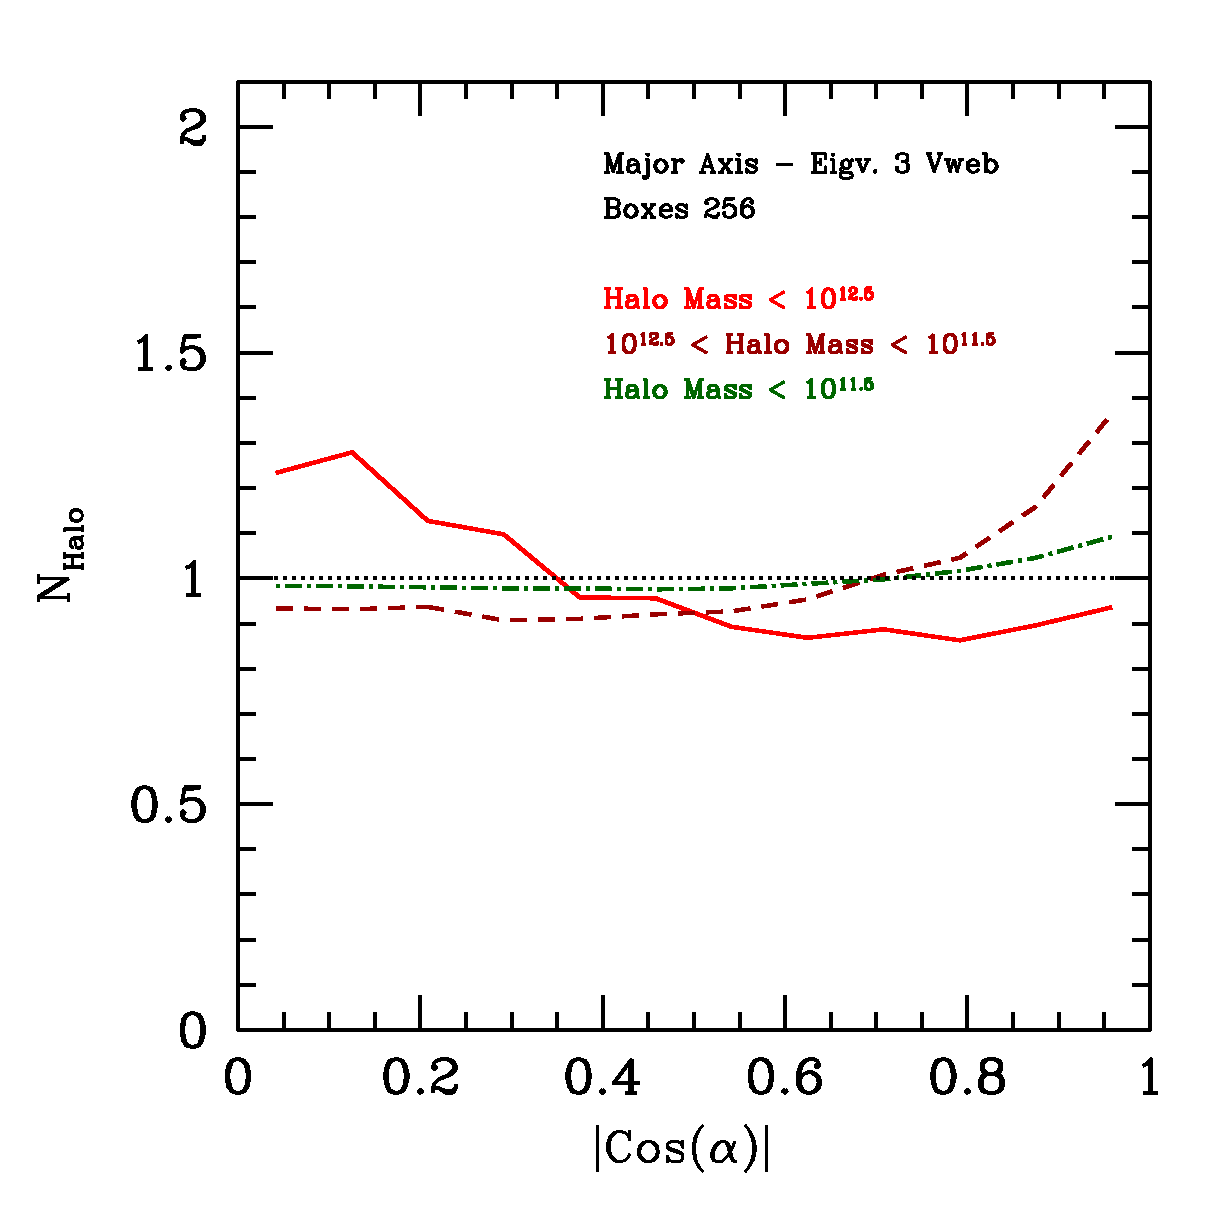
\includegraphics[width=0.30\textwidth]{../plot2/Ax1_VT/256_AX1_V3.ps}
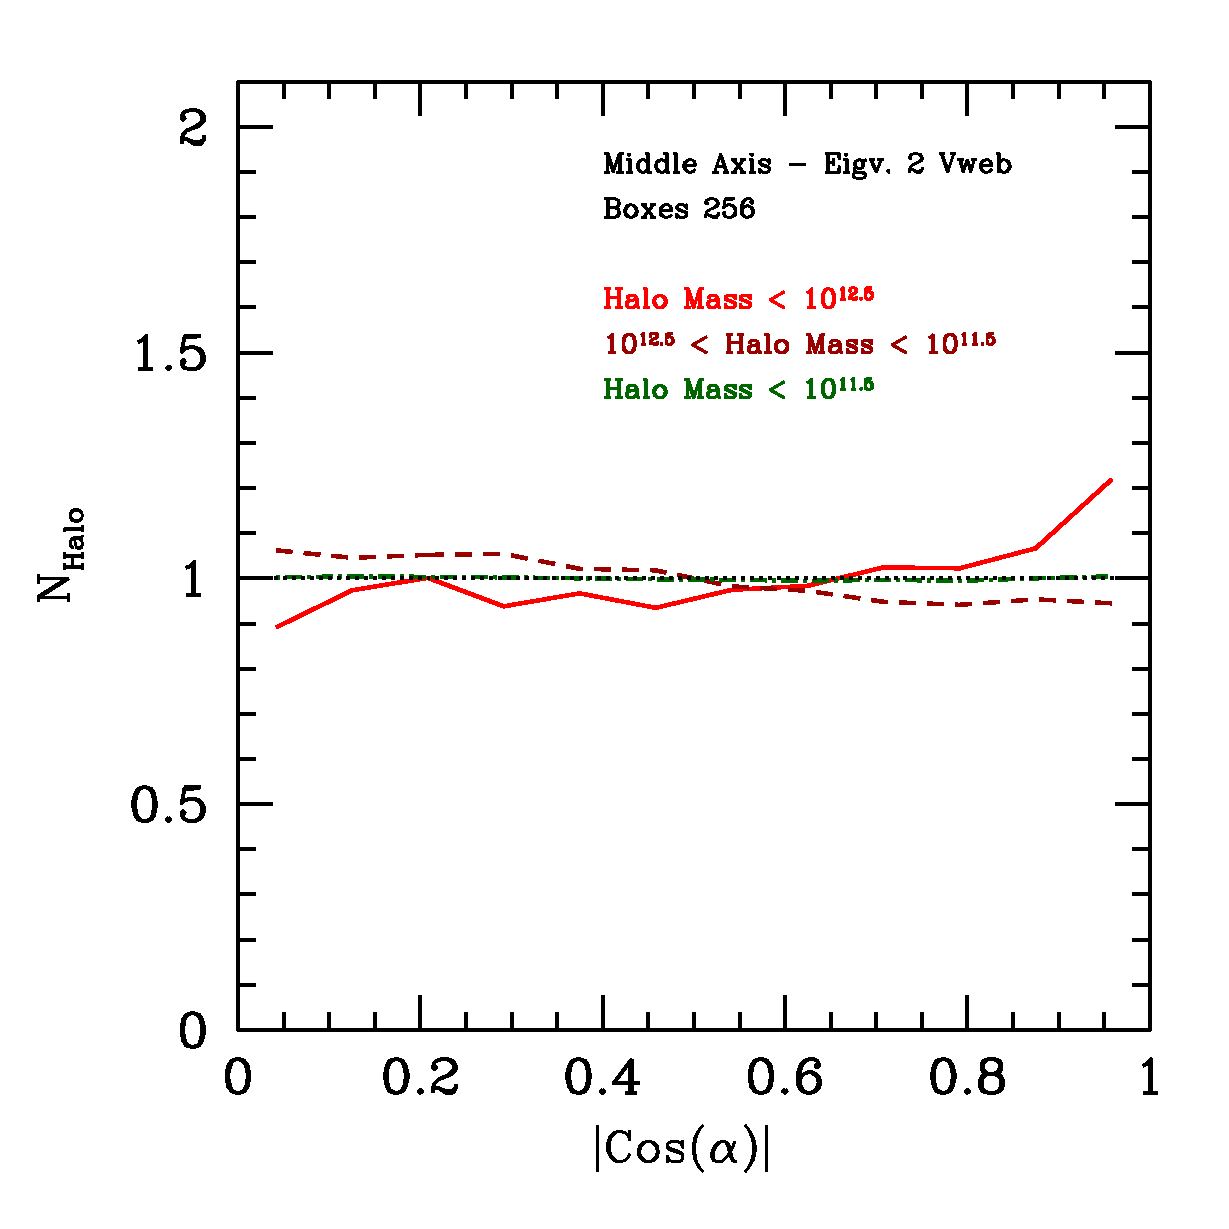
\includegraphics[width=0.30\textwidth]{../plot2/Ax2_VT/256_AX2_V2.ps}
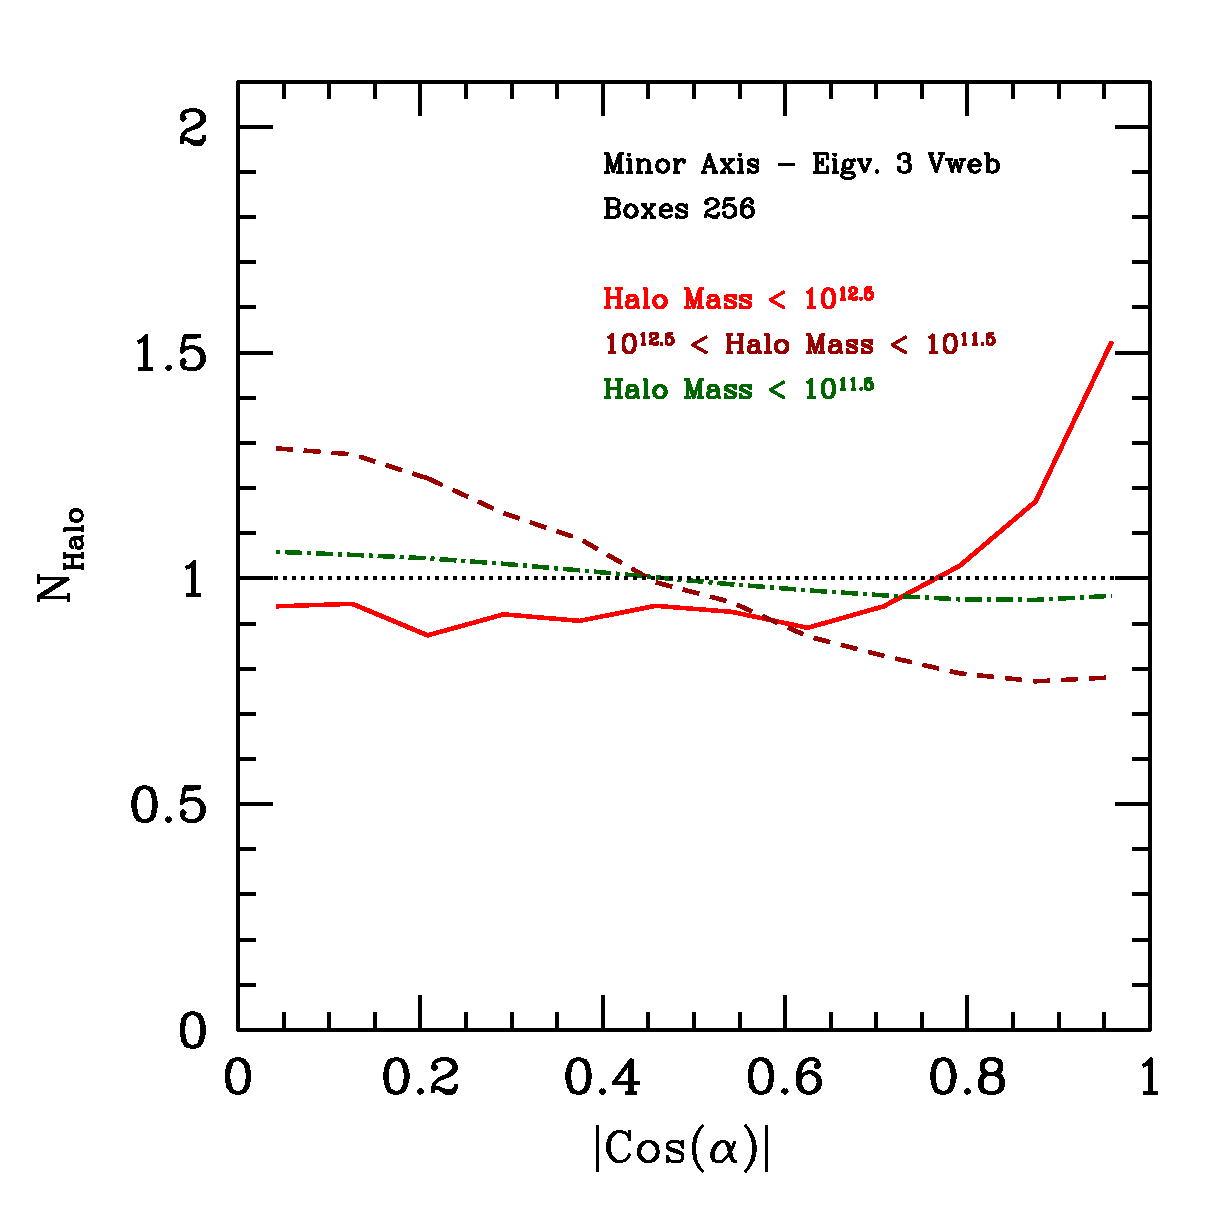
\includegraphics[width=0.30\textwidth]{../plot2/Ax3_VT/256_AX3_V3.ps}
\caption{Shape alignment for the vweb at $256^3$ resolution.}
\end{figure*}

\begin{figure*}
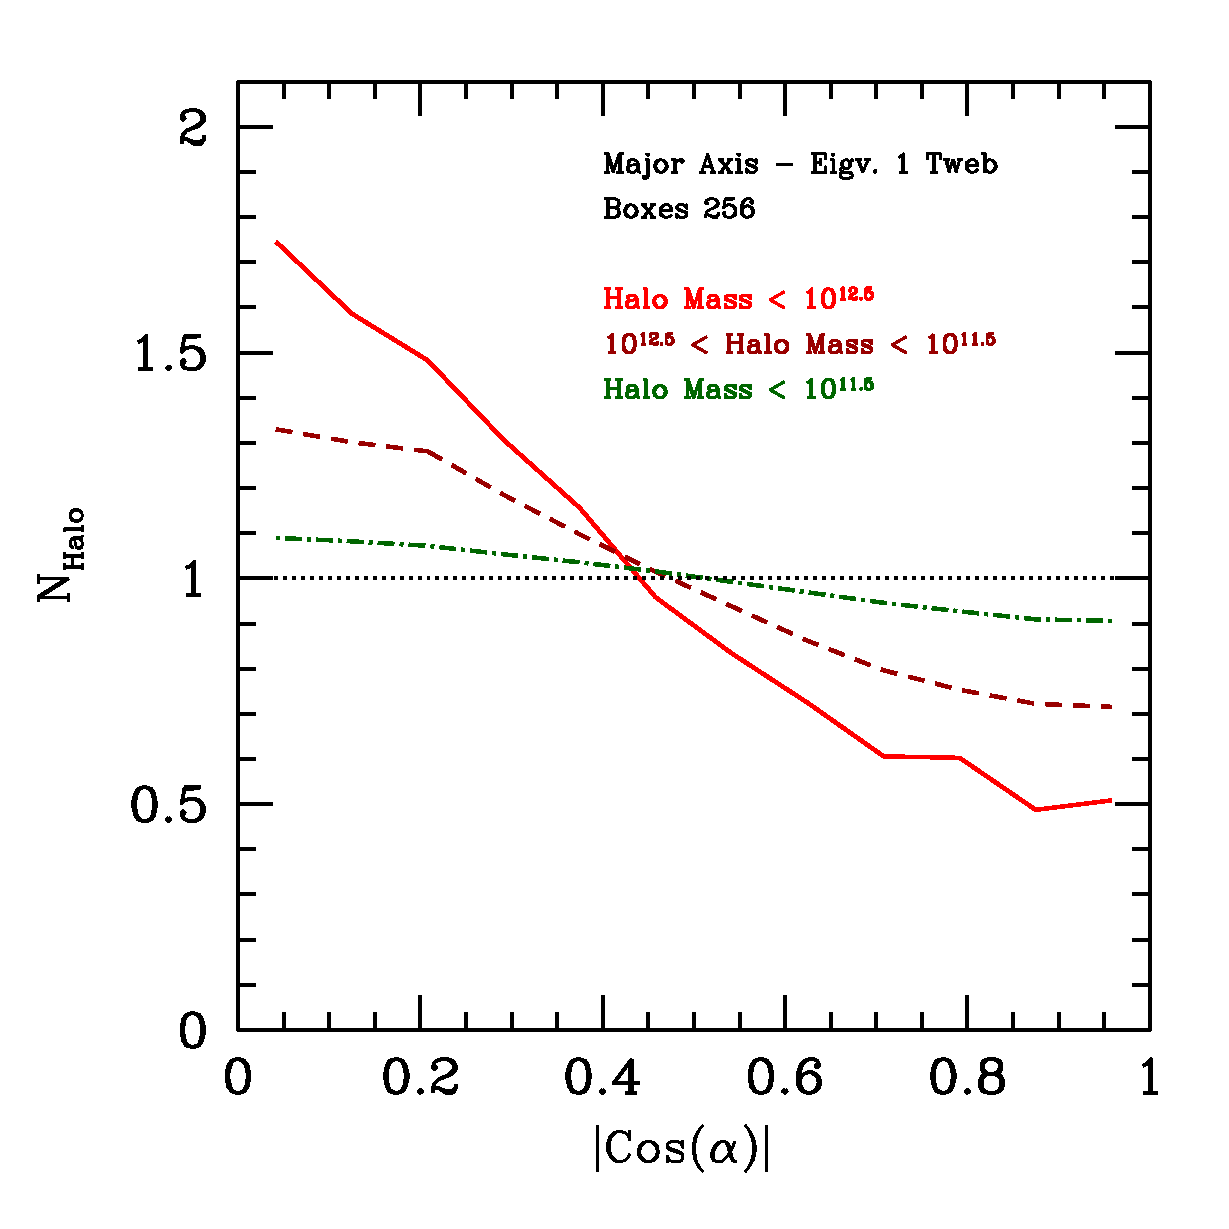
\includegraphics[width=0.30\textwidth]{../plot2/Ax1_VT/256_AX1_T1.ps}
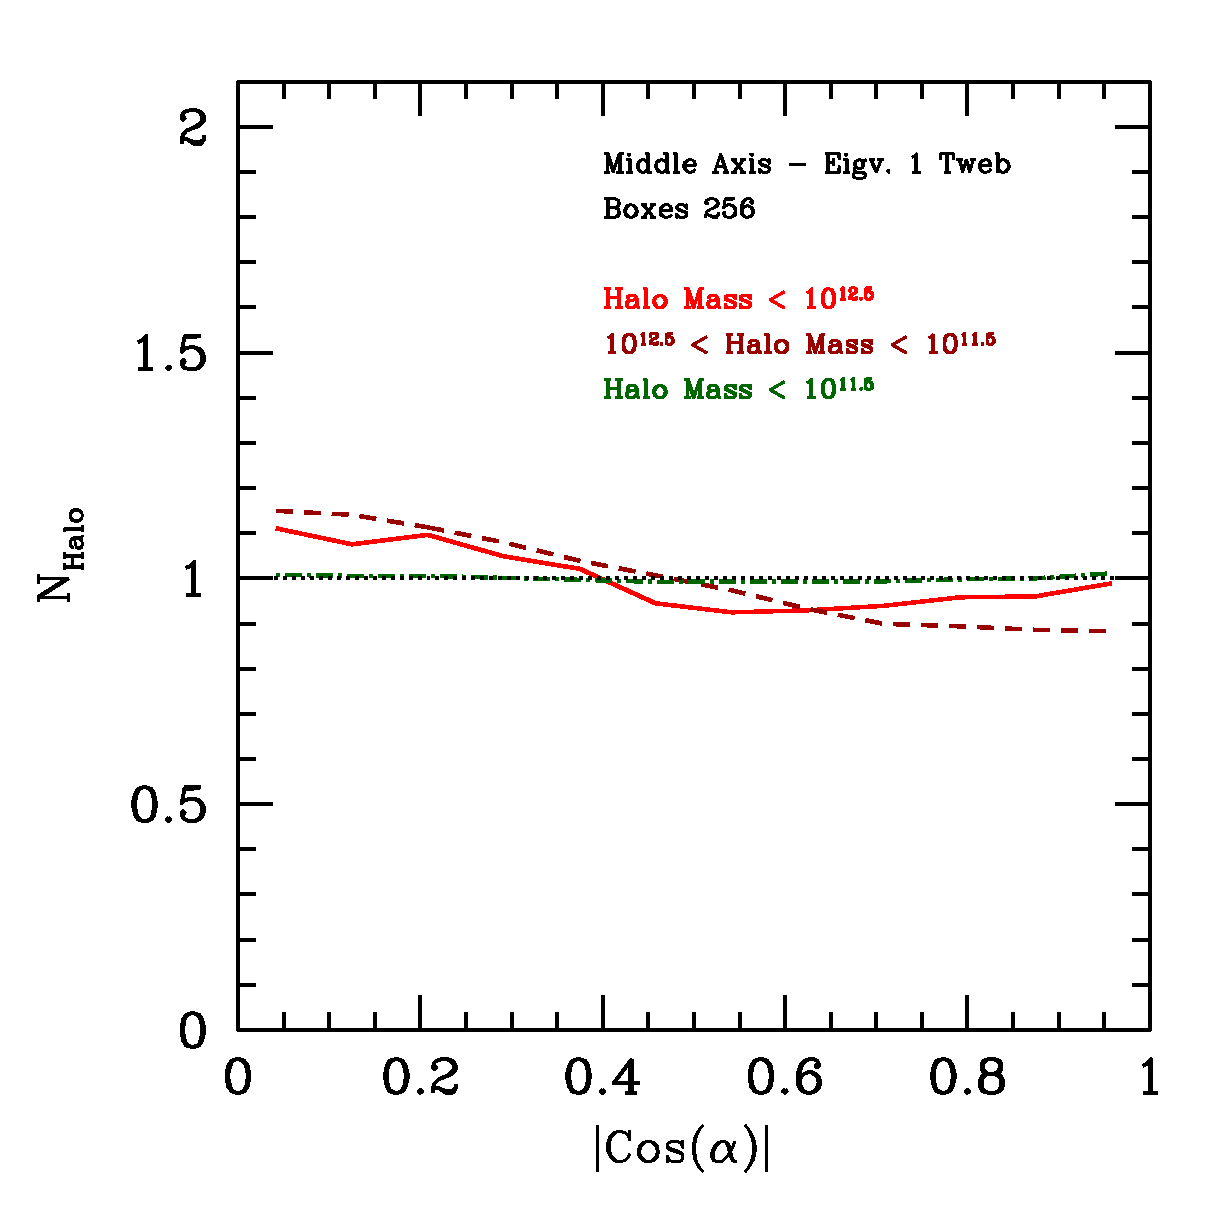
\includegraphics[width=0.30\textwidth]{../plot2/Ax2_VT/256_AX2_T1.ps}
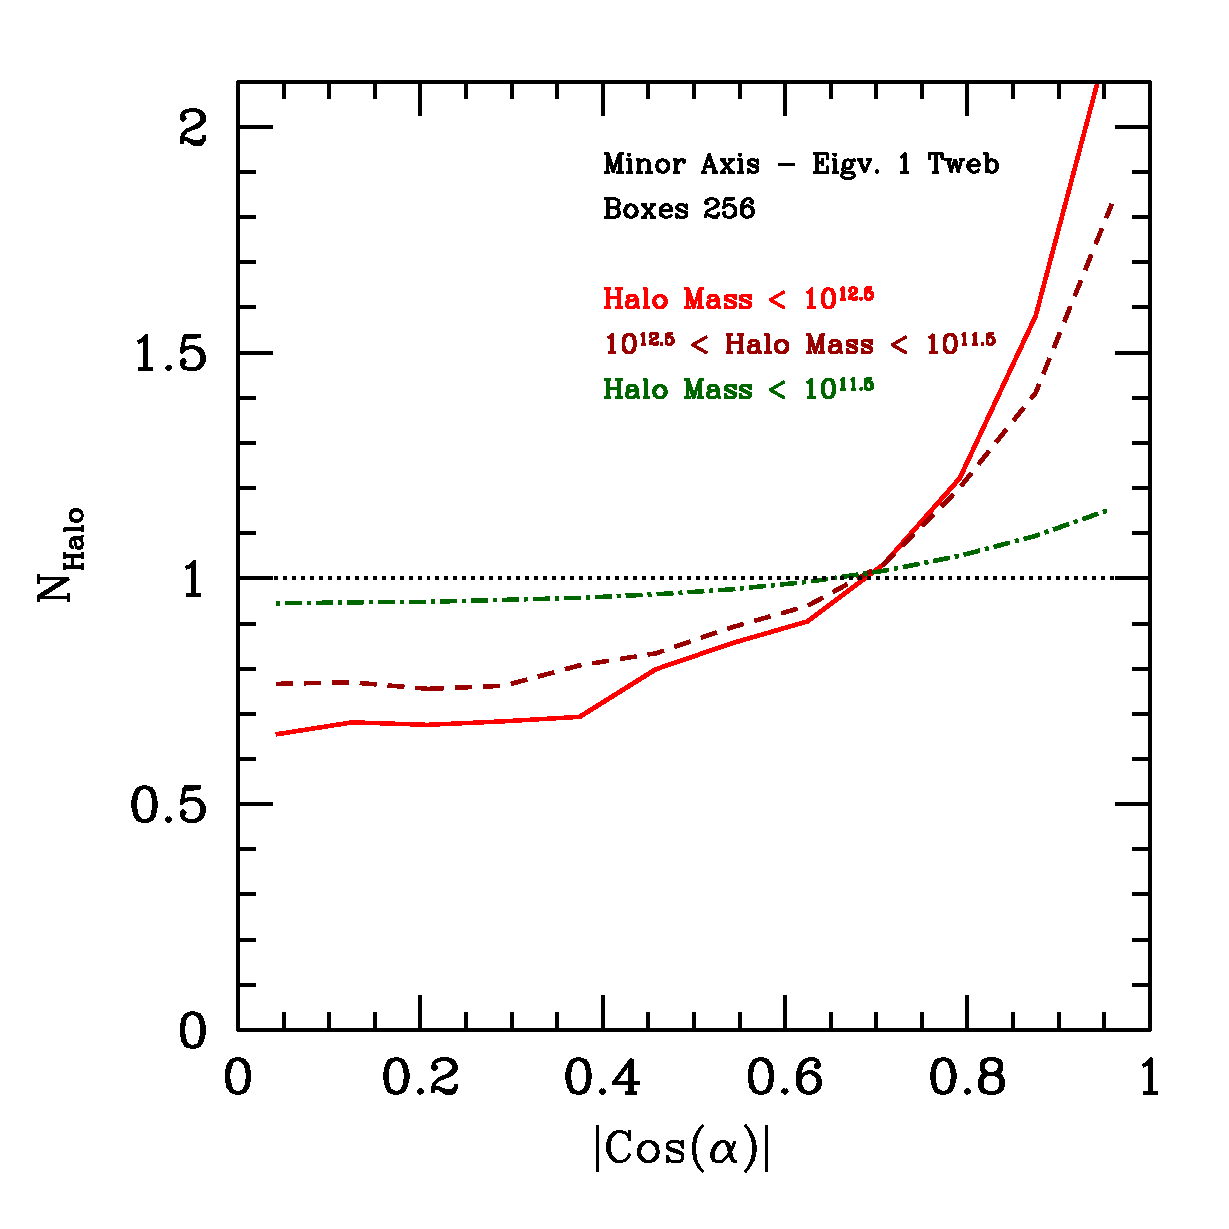
\includegraphics[width=0.30\textwidth]{../plot2/Ax3_VT/256_AX3_T1.ps}
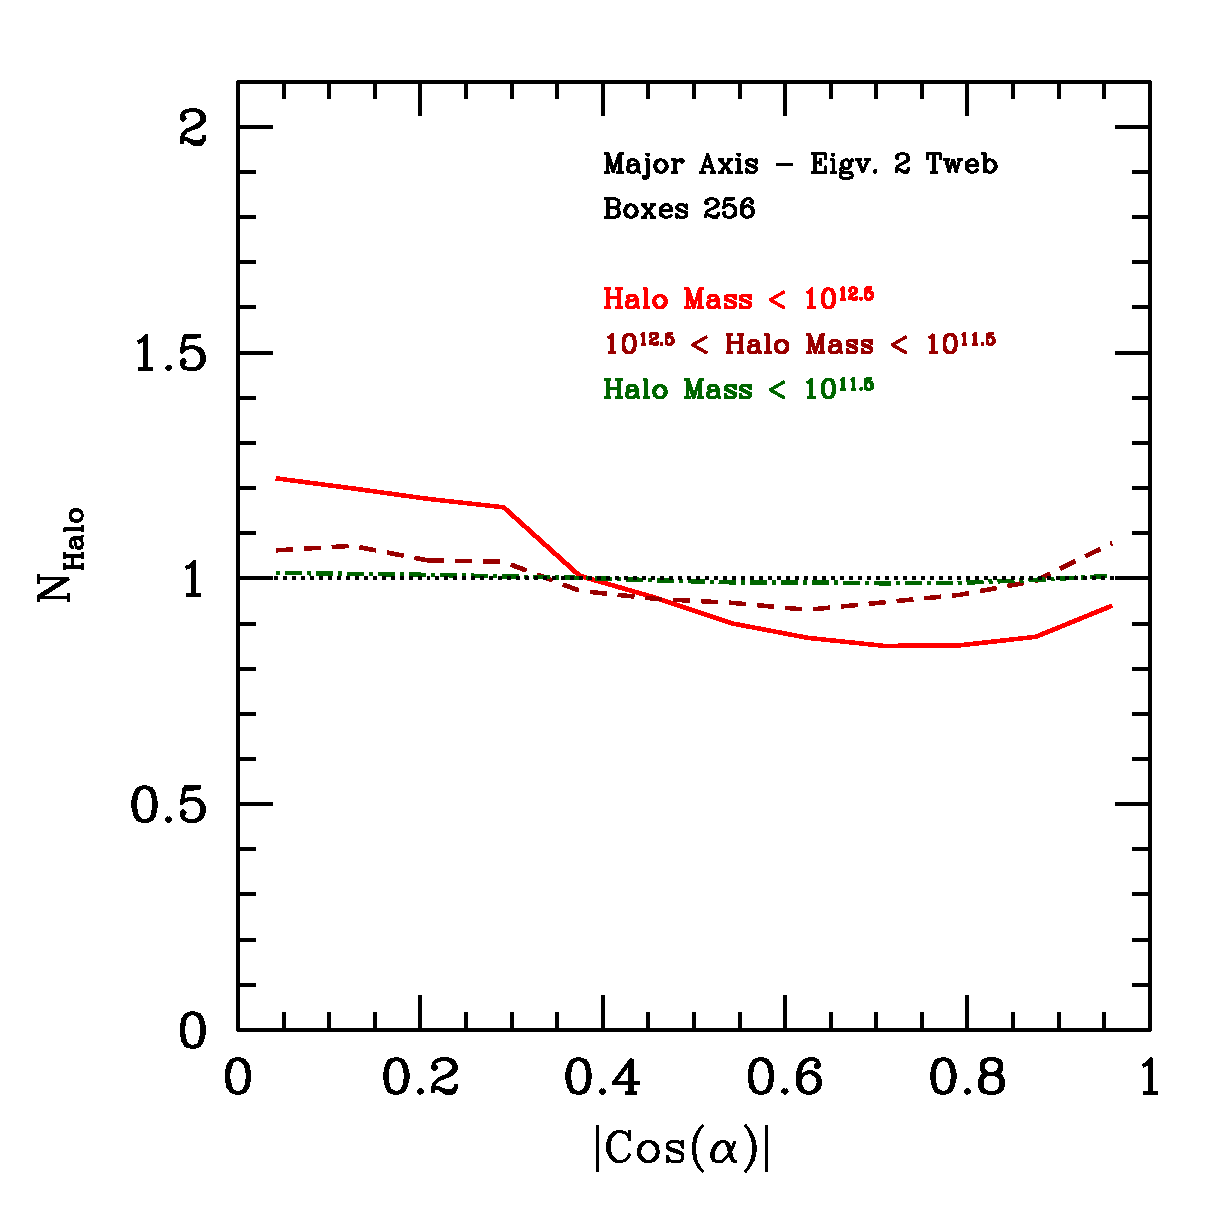
\includegraphics[width=0.30\textwidth]{../plot2/Ax1_VT/256_AX1_T2.ps}
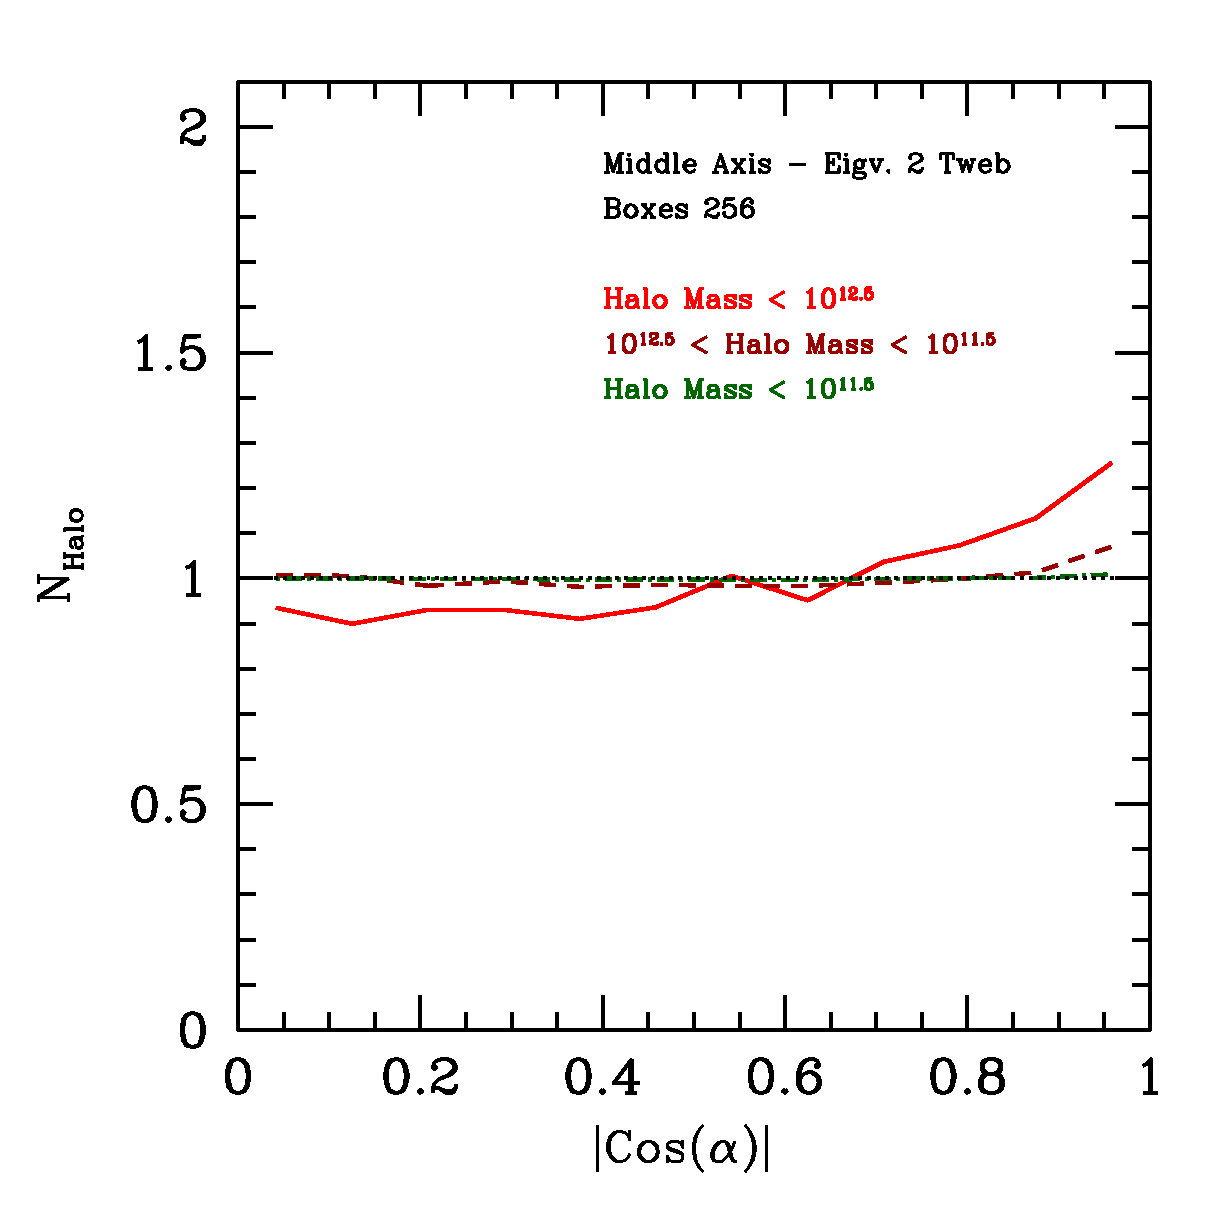
\includegraphics[width=0.30\textwidth]{../plot2/Ax2_VT/256_AX2_T2.ps}
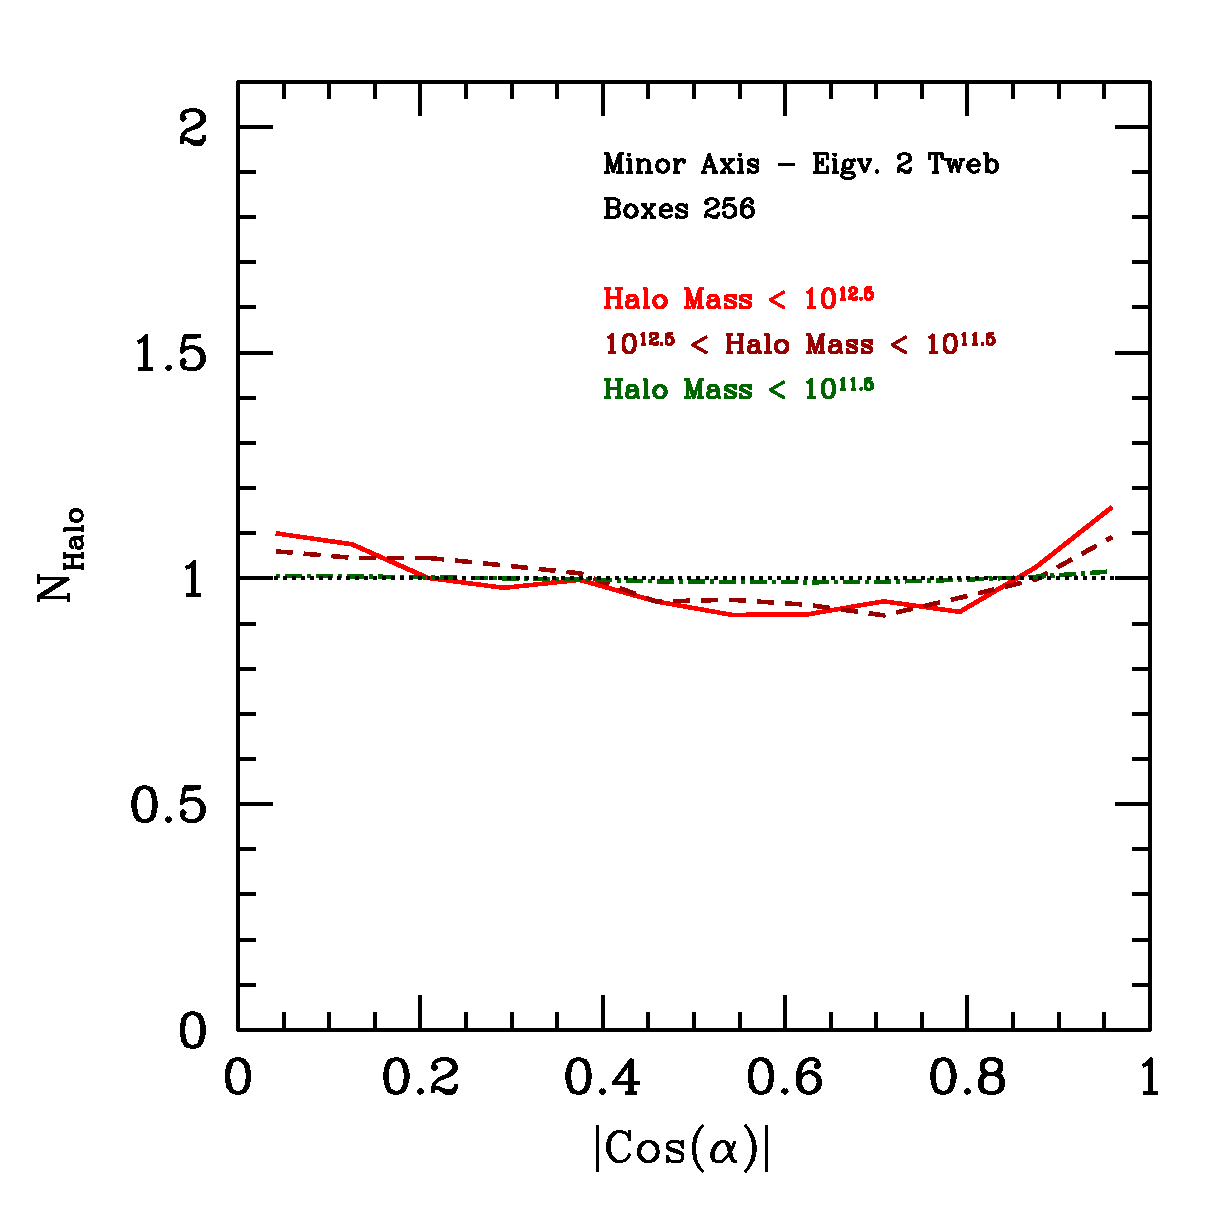
\includegraphics[width=0.30\textwidth]{../plot2/Ax3_VT/256_AX3_T2.ps}
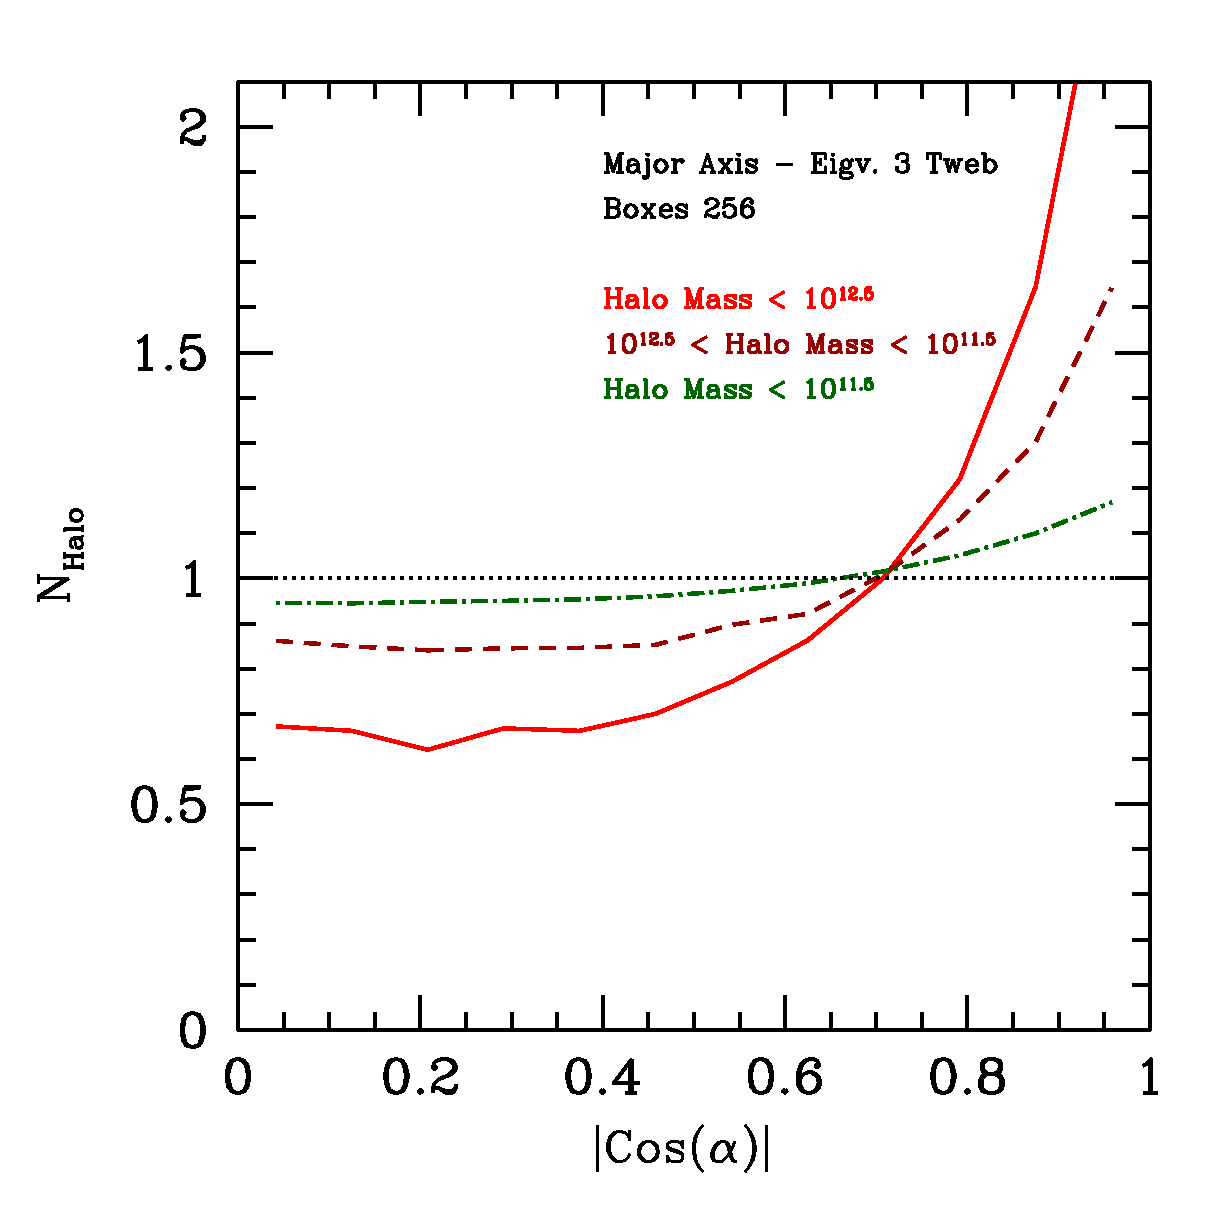
\includegraphics[width=0.30\textwidth]{../plot2/Ax1_VT/256_AX1_T3.ps}
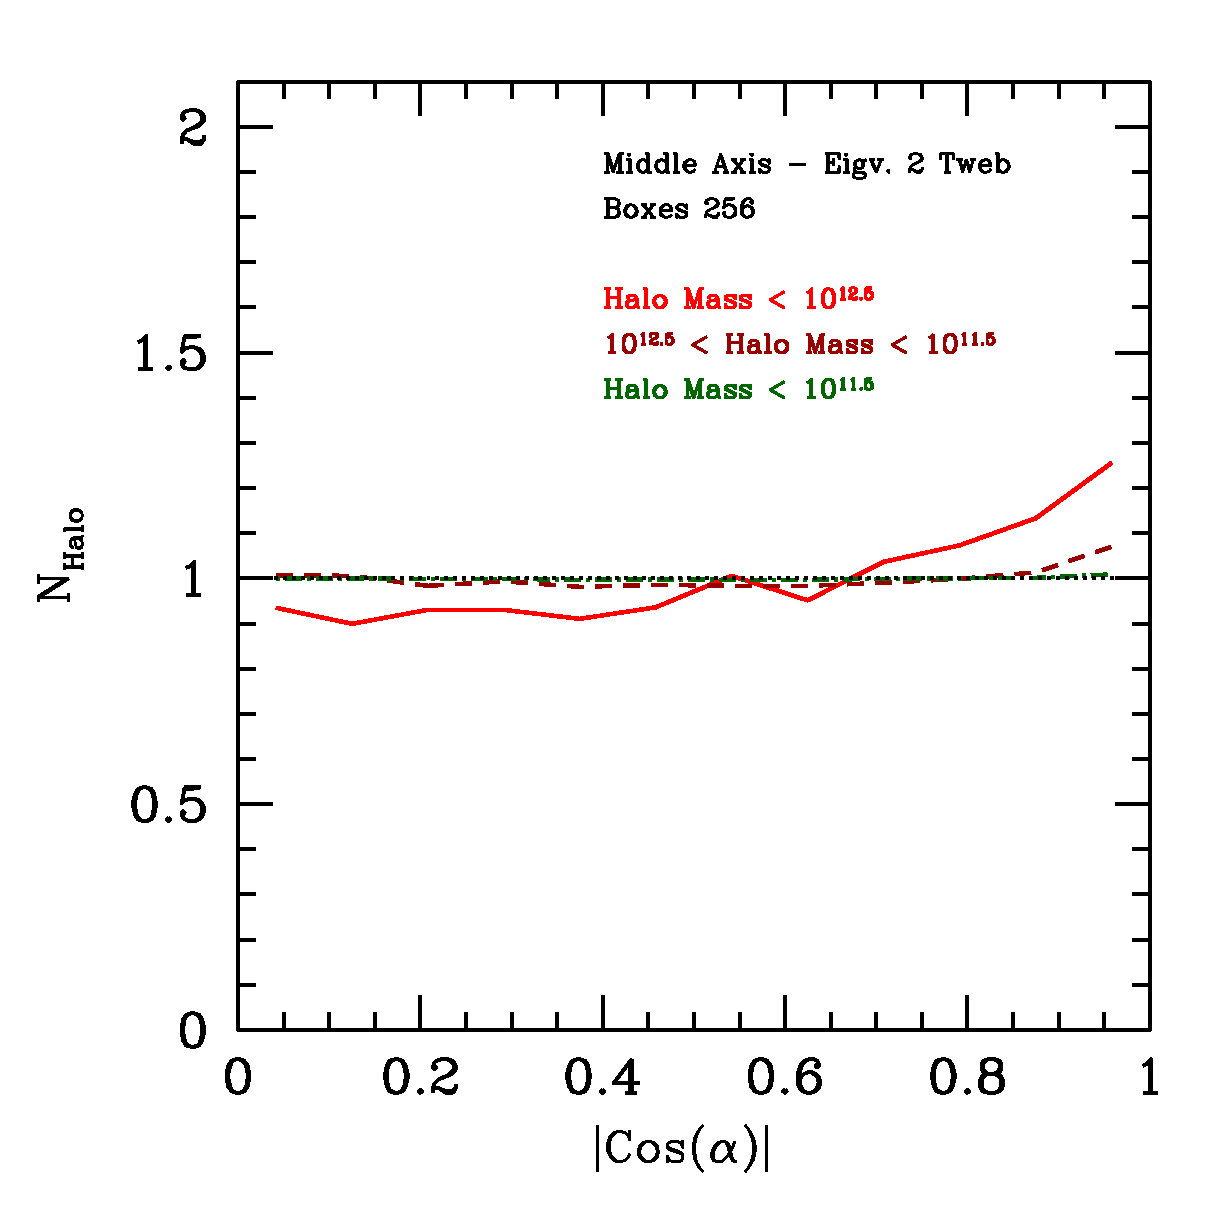
\includegraphics[width=0.30\textwidth]{../plot2/Ax2_VT/256_AX2_T2.ps}
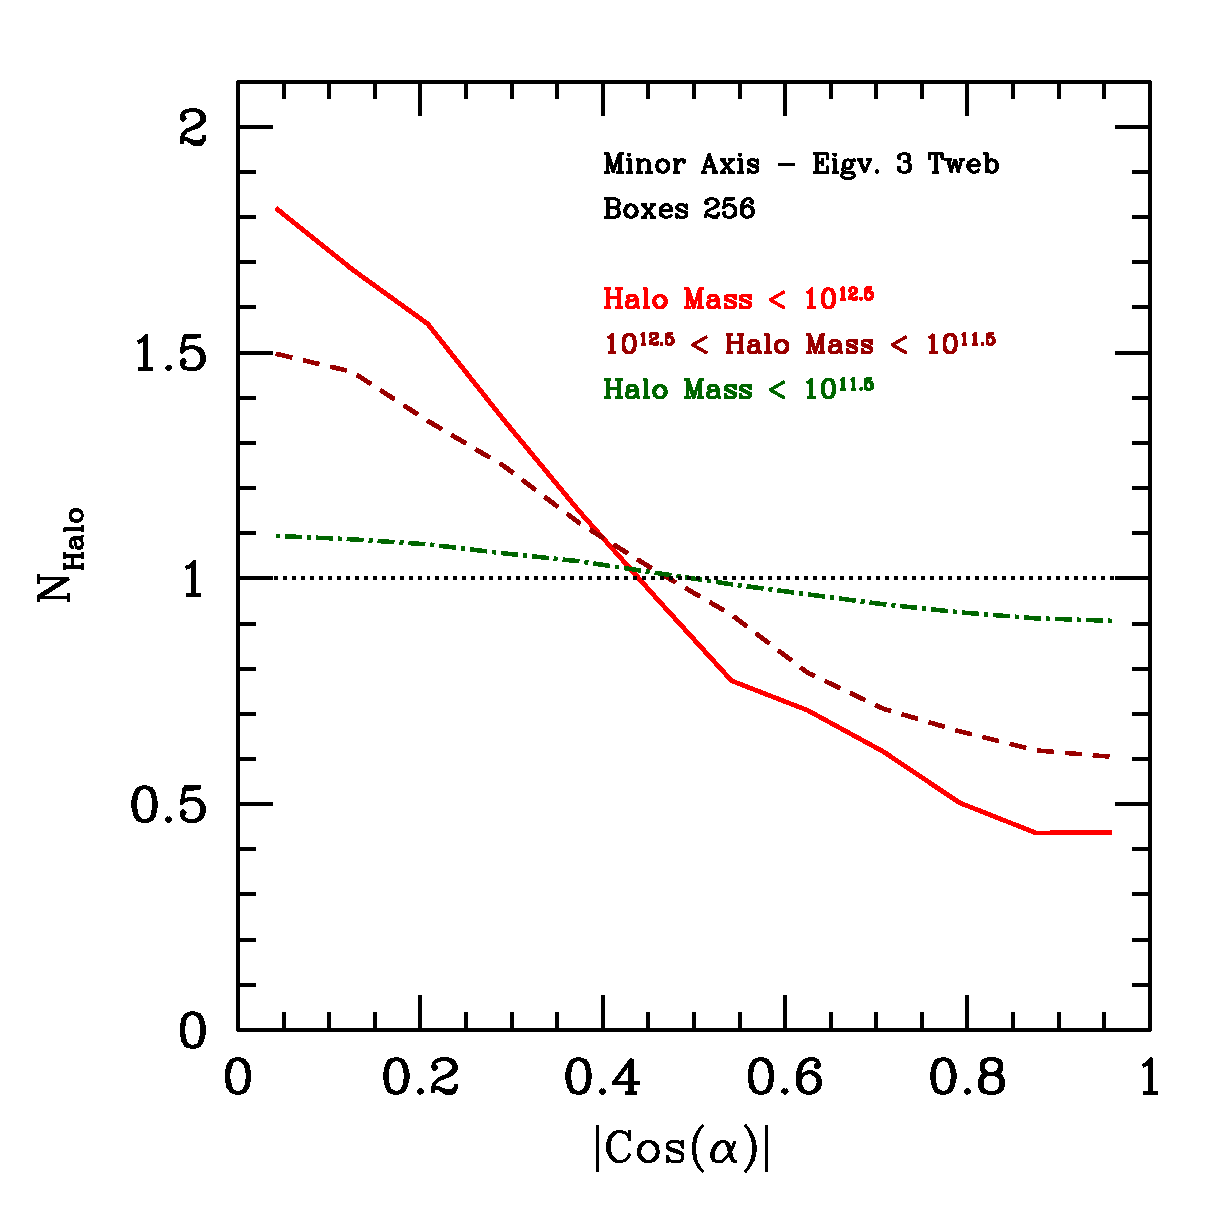
\includegraphics[width=0.30\textwidth]{../plot2/Ax3_VT/256_AX3_T3.ps}
\caption{Shape alignment for the tweb at $256^3$ resolution.}
\end{figure*}


\begin{figure*}
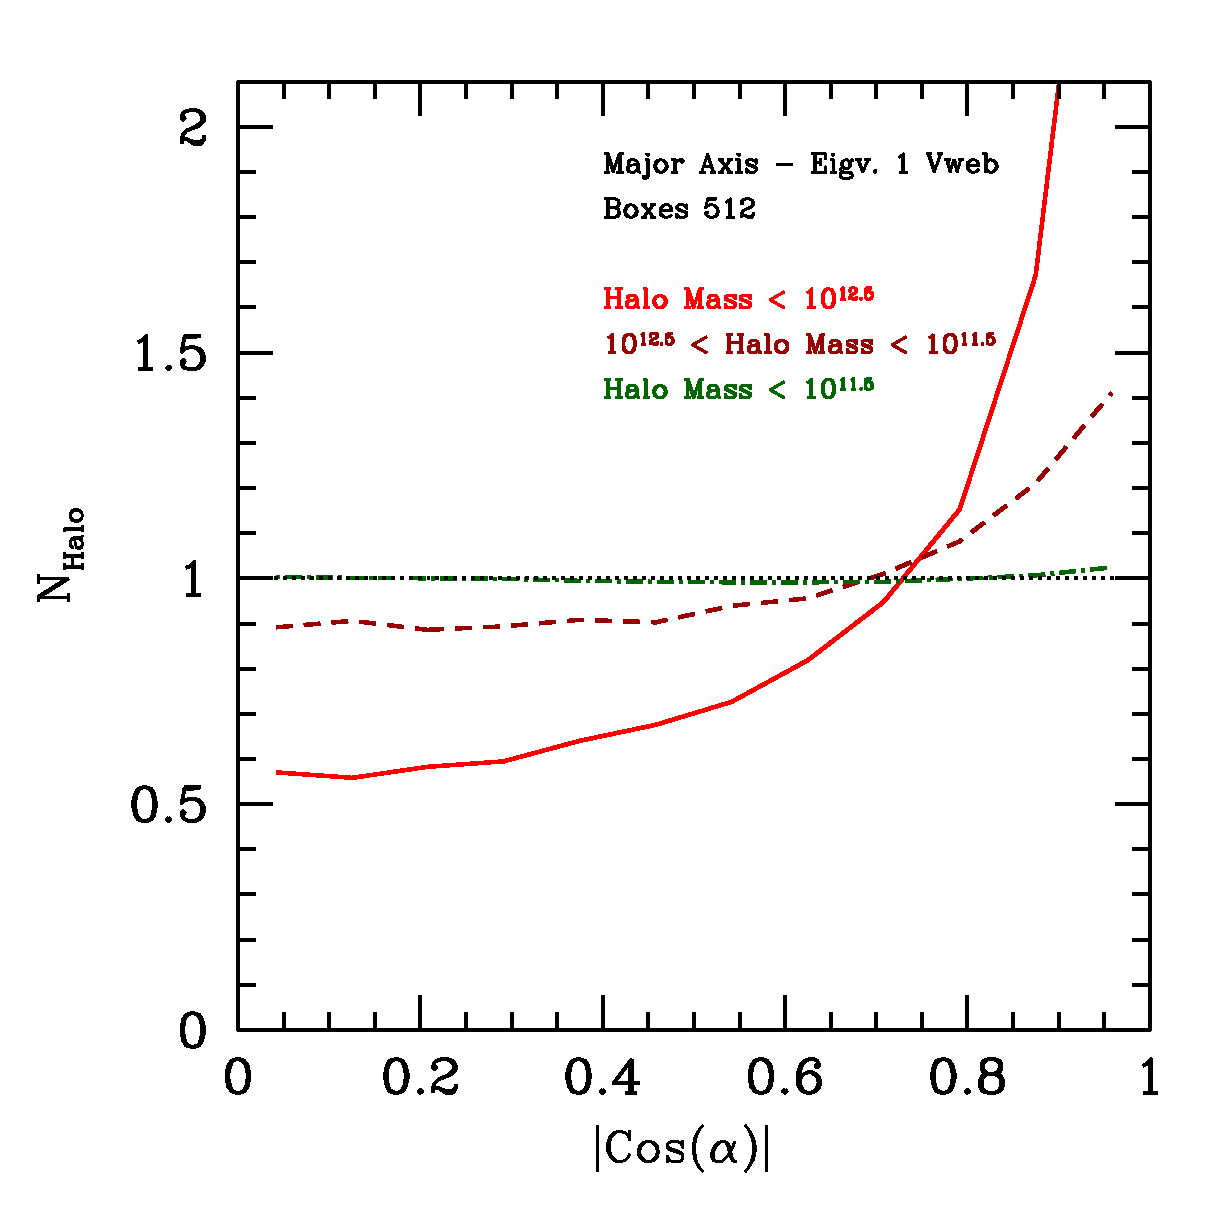
\includegraphics[width=0.30\textwidth]{../plot2/Ax1_VT/512_AX1_V1.ps}
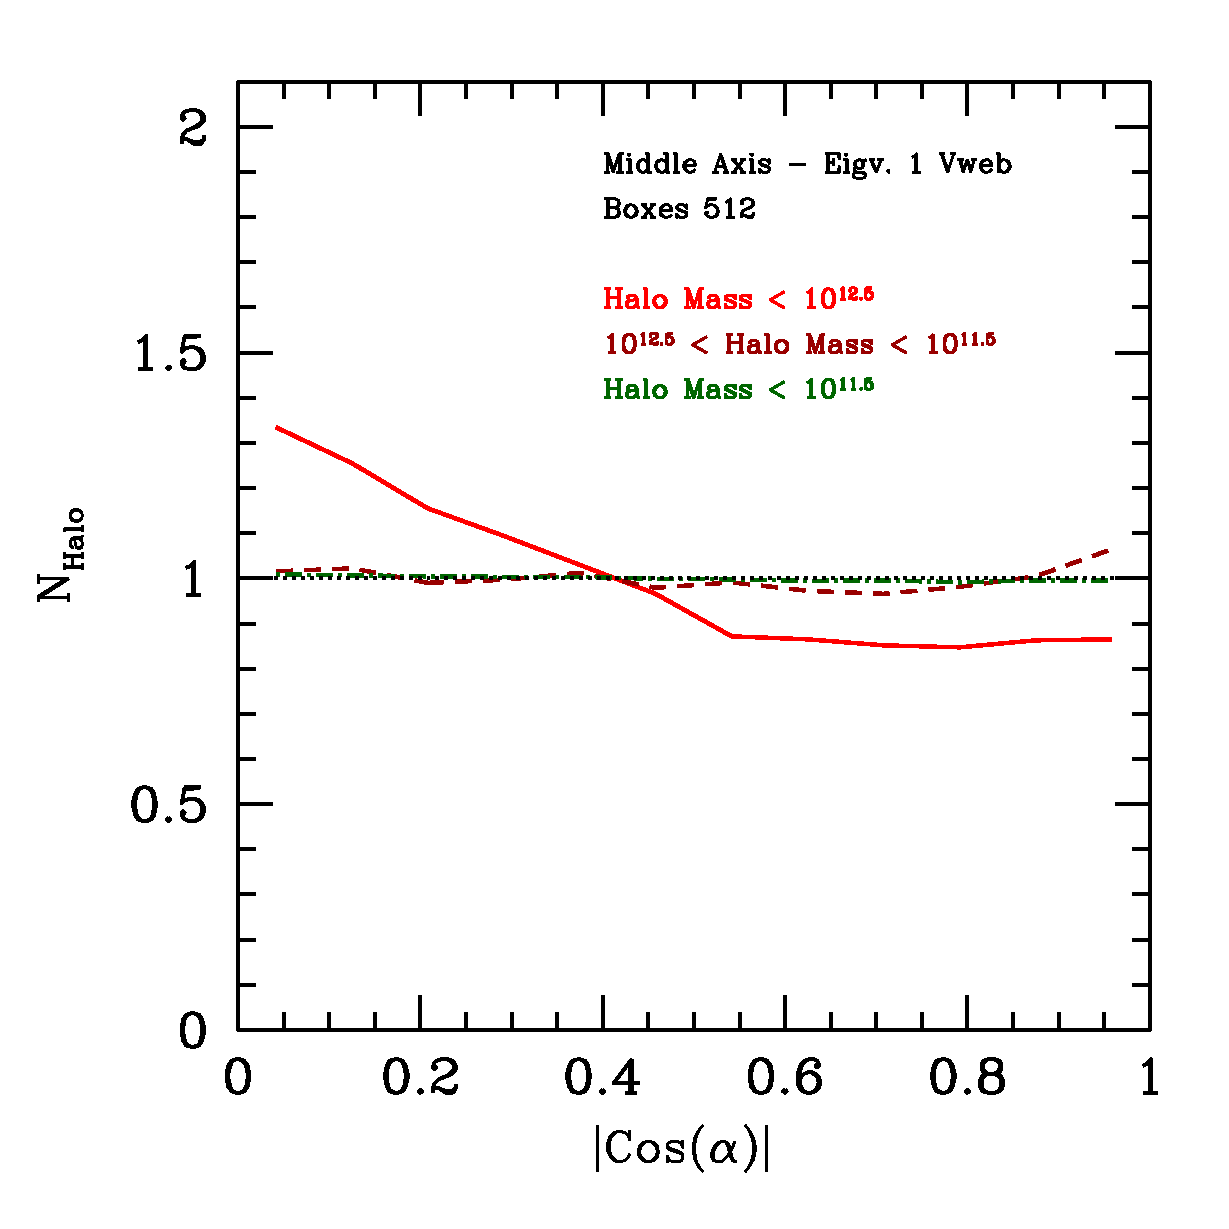
\includegraphics[width=0.30\textwidth]{../plot2/Ax2_VT/512_AX2_V1.ps}
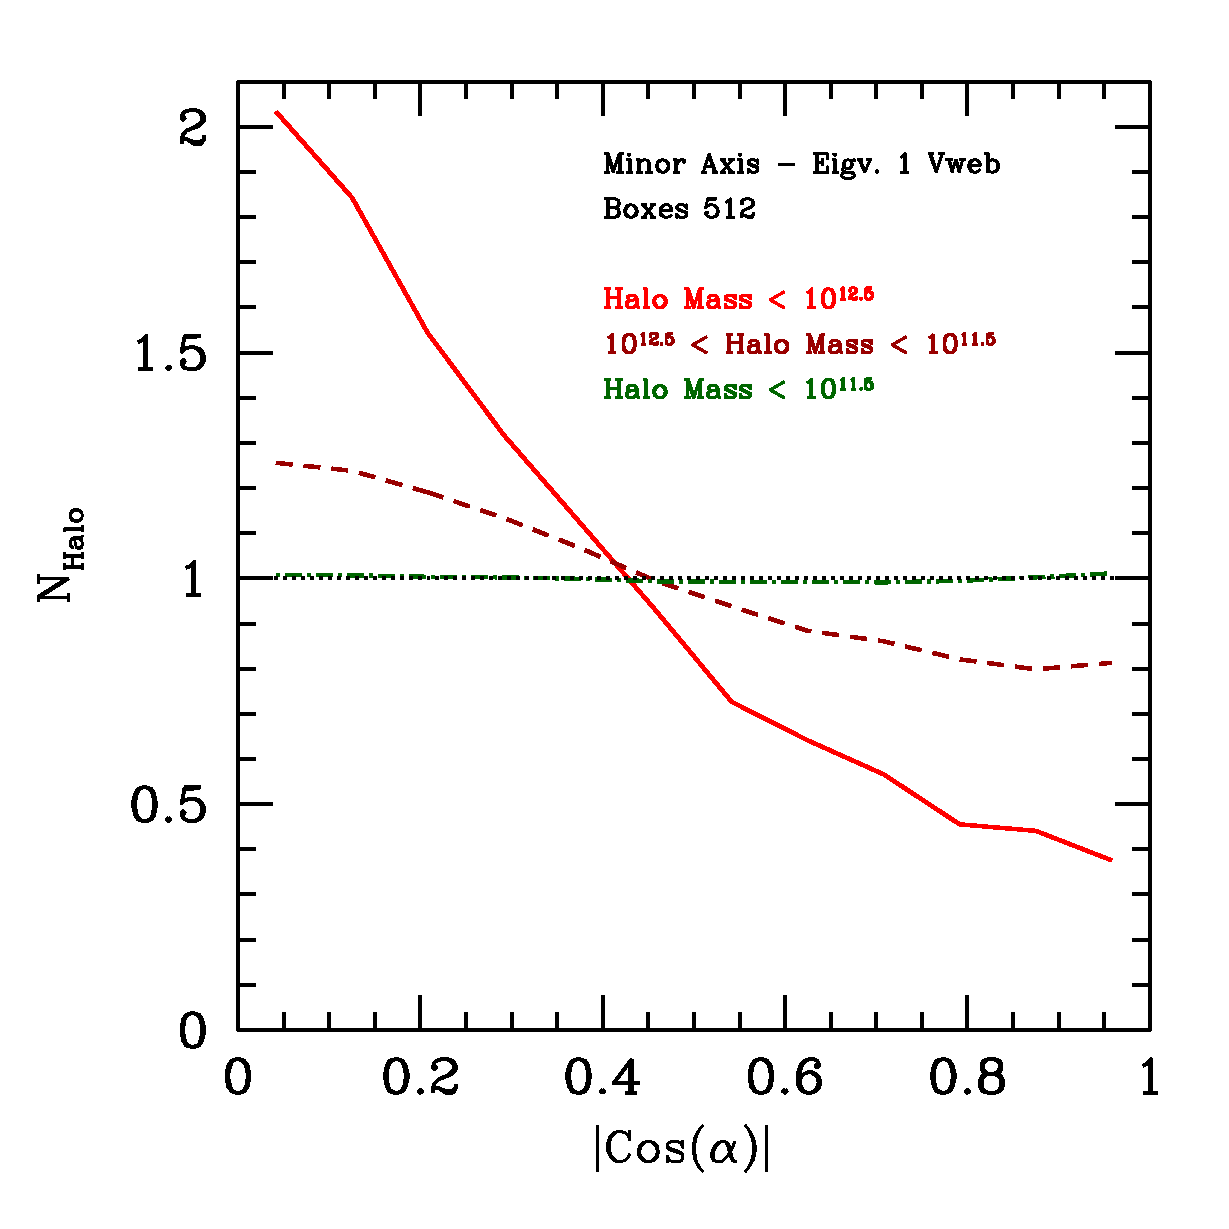
\includegraphics[width=0.30\textwidth]{../plot2/Ax3_VT/512_AX3_V1.ps}
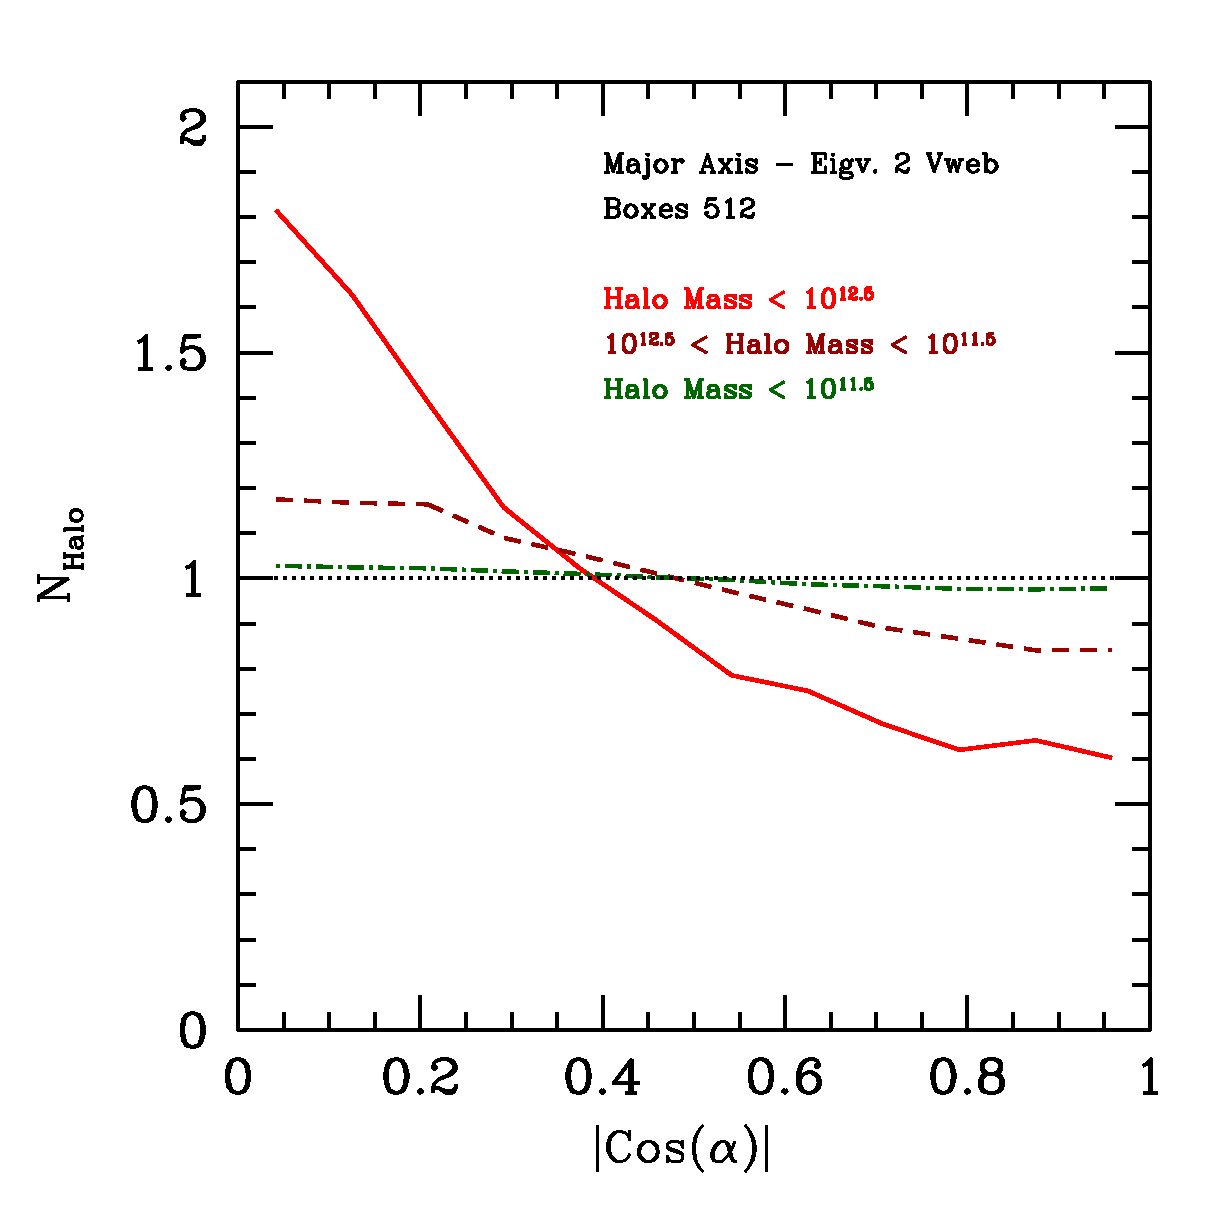
\includegraphics[width=0.30\textwidth]{../plot2/Ax1_VT/512_AX1_V2.ps}
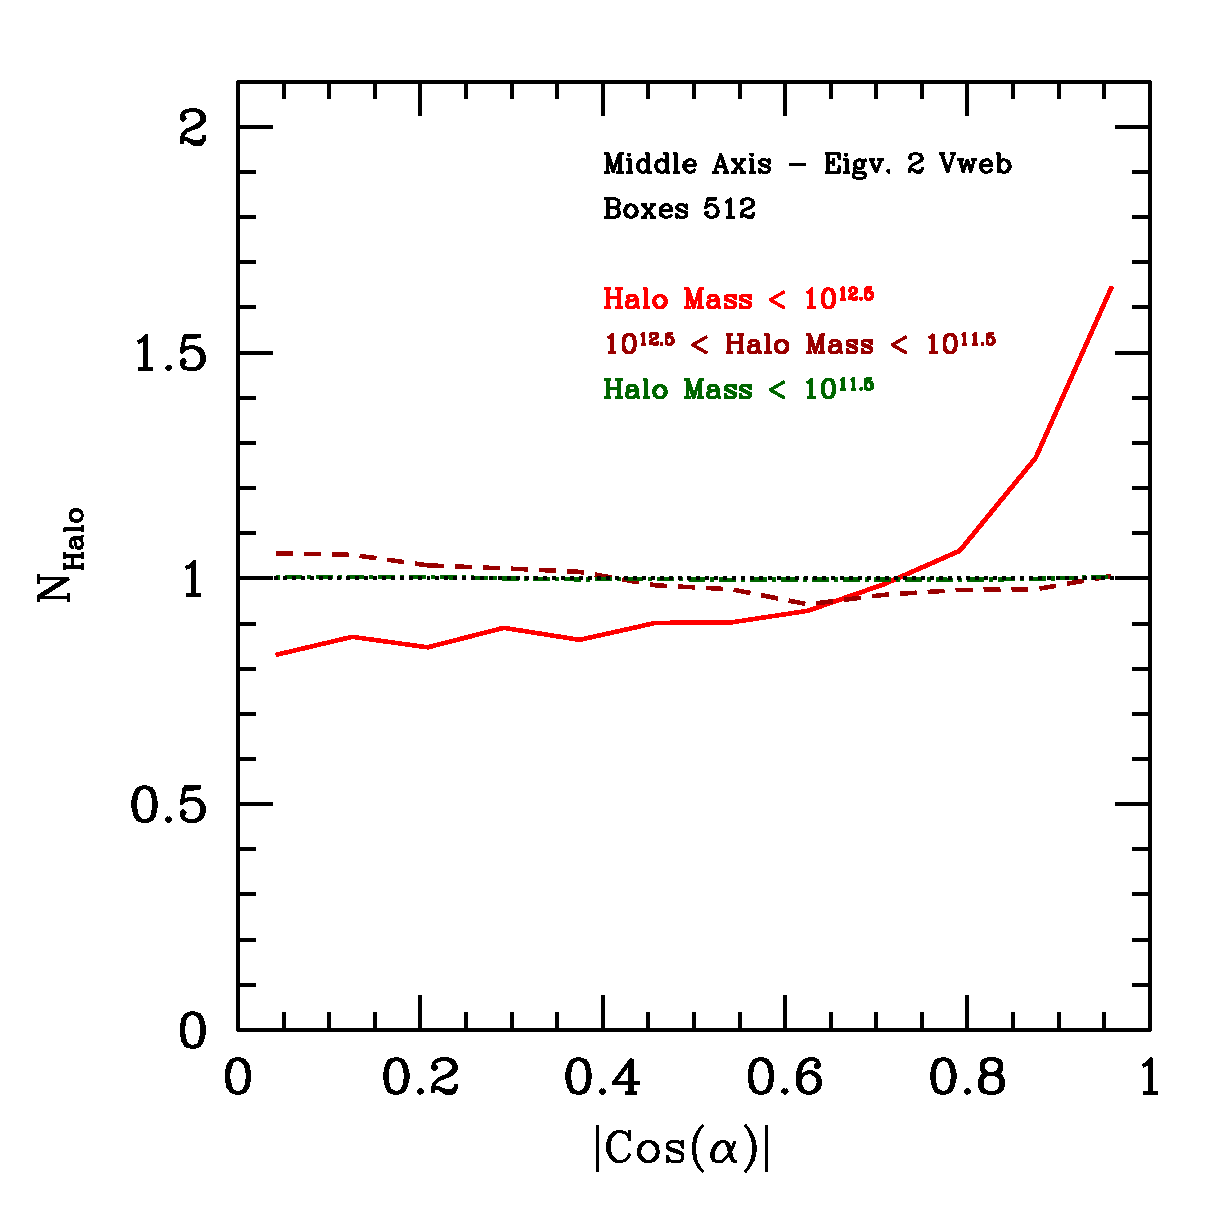
\includegraphics[width=0.30\textwidth]{../plot2/Ax2_VT/512_AX2_V2.ps}
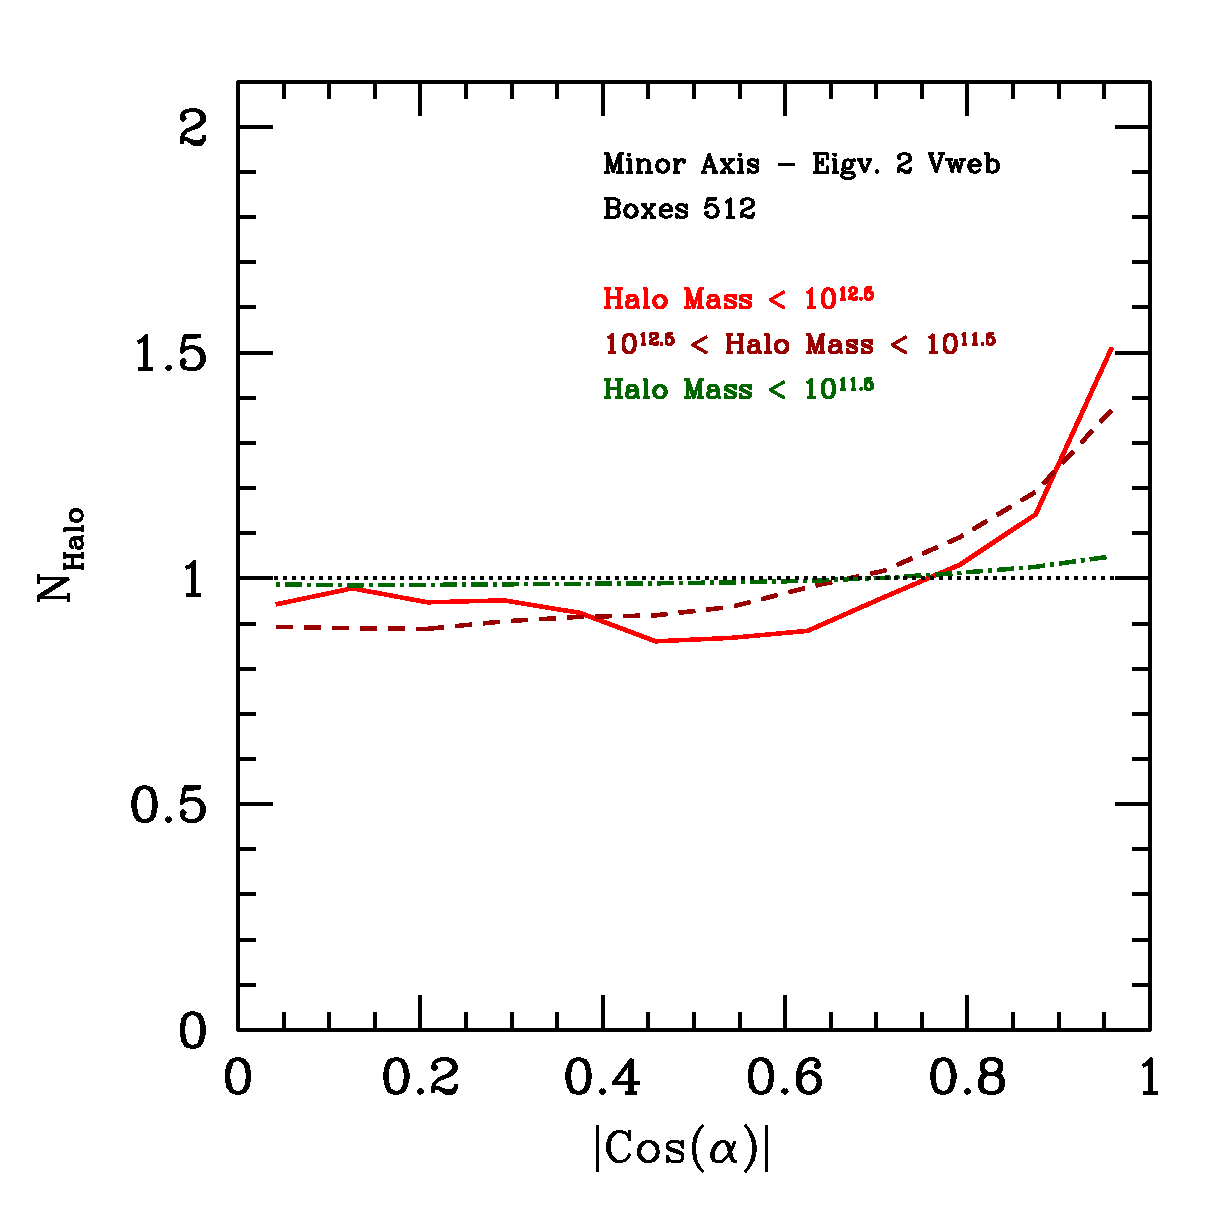
\includegraphics[width=0.30\textwidth]{../plot2/Ax3_VT/512_AX3_V2.ps}
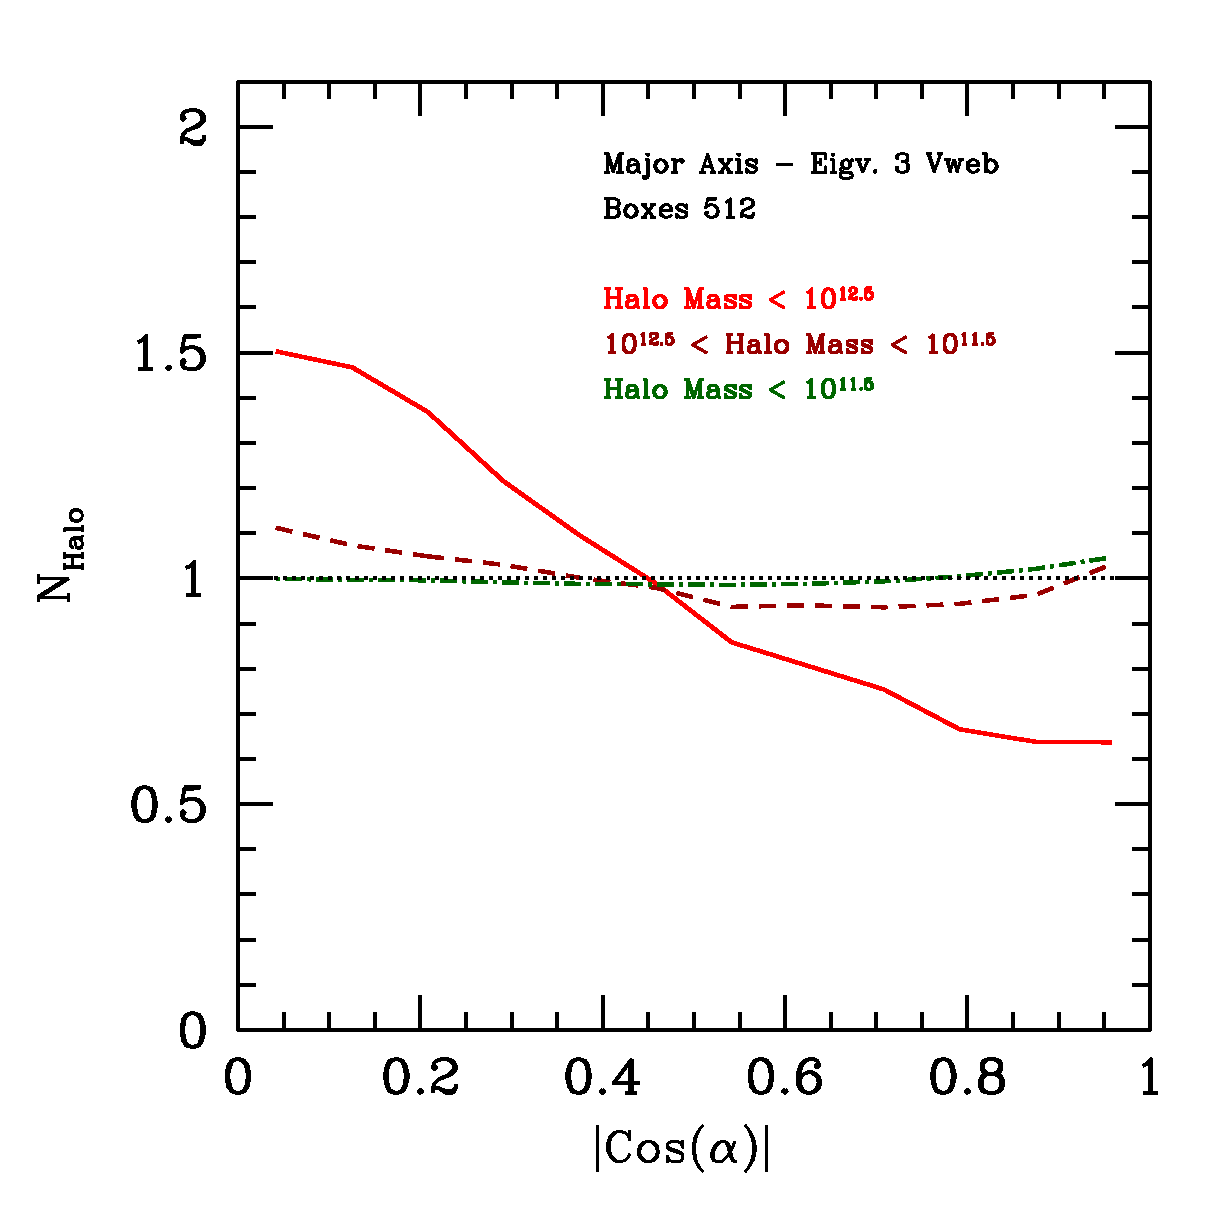
\includegraphics[width=0.30\textwidth]{../plot2/Ax1_VT/512_AX1_V3.ps}
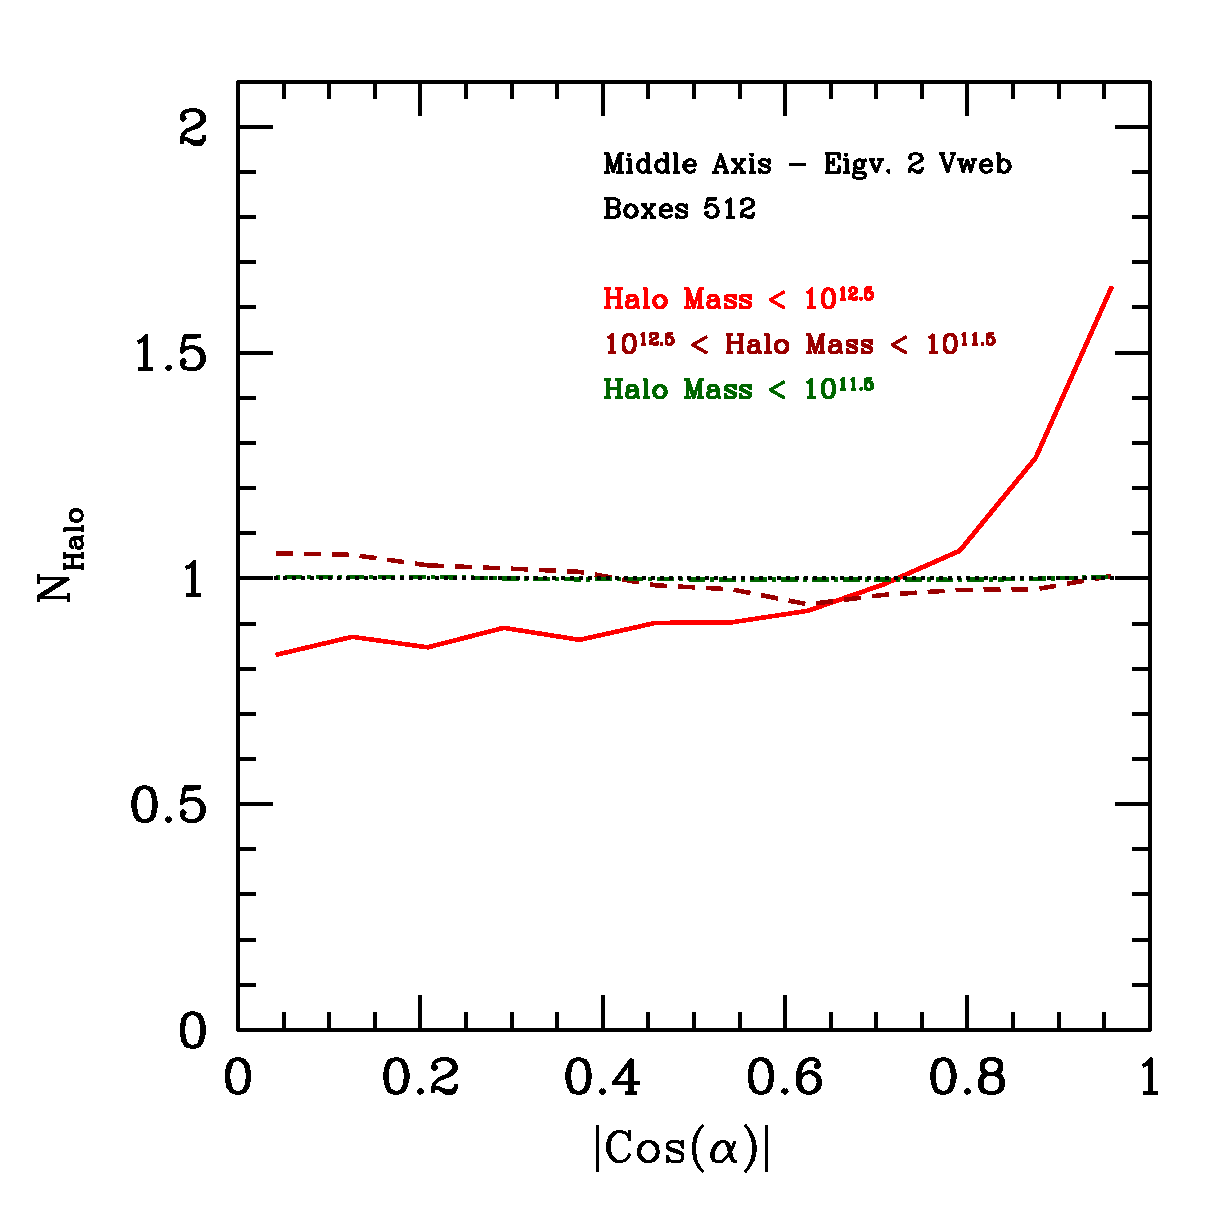
\includegraphics[width=0.30\textwidth]{../plot2/Ax2_VT/512_AX2_V2.ps}
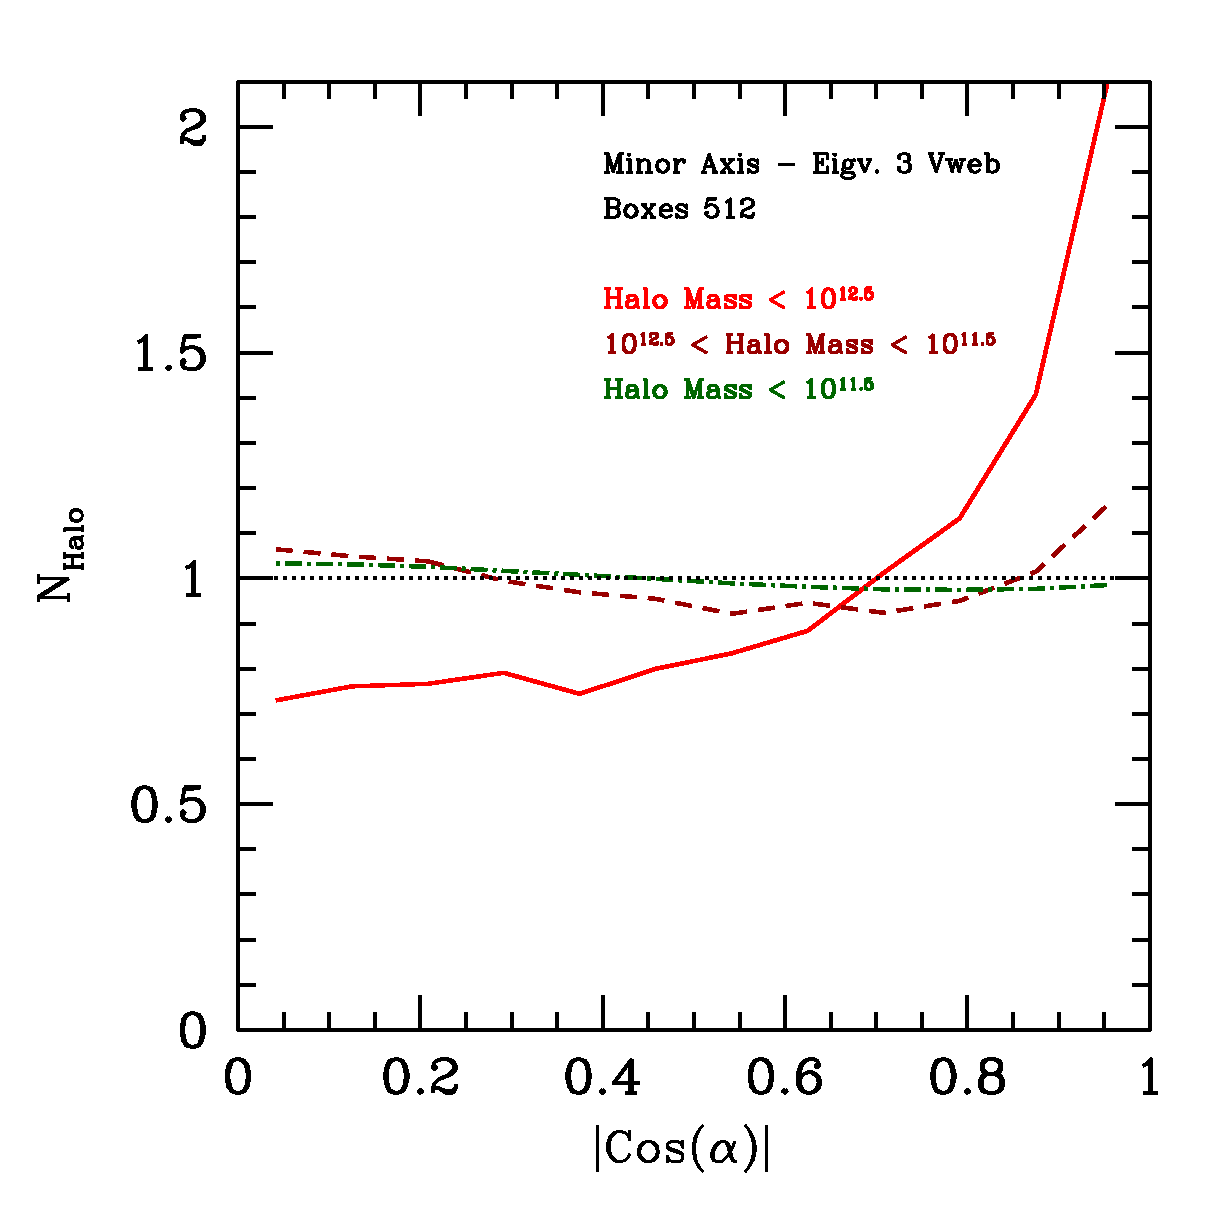
\includegraphics[width=0.30\textwidth]{../plot2/Ax3_VT/512_AX3_V3.ps}
\caption{Shape alignment for the vweb at $512^3$ resolution.}
\end{figure*}

\begin{figure*}
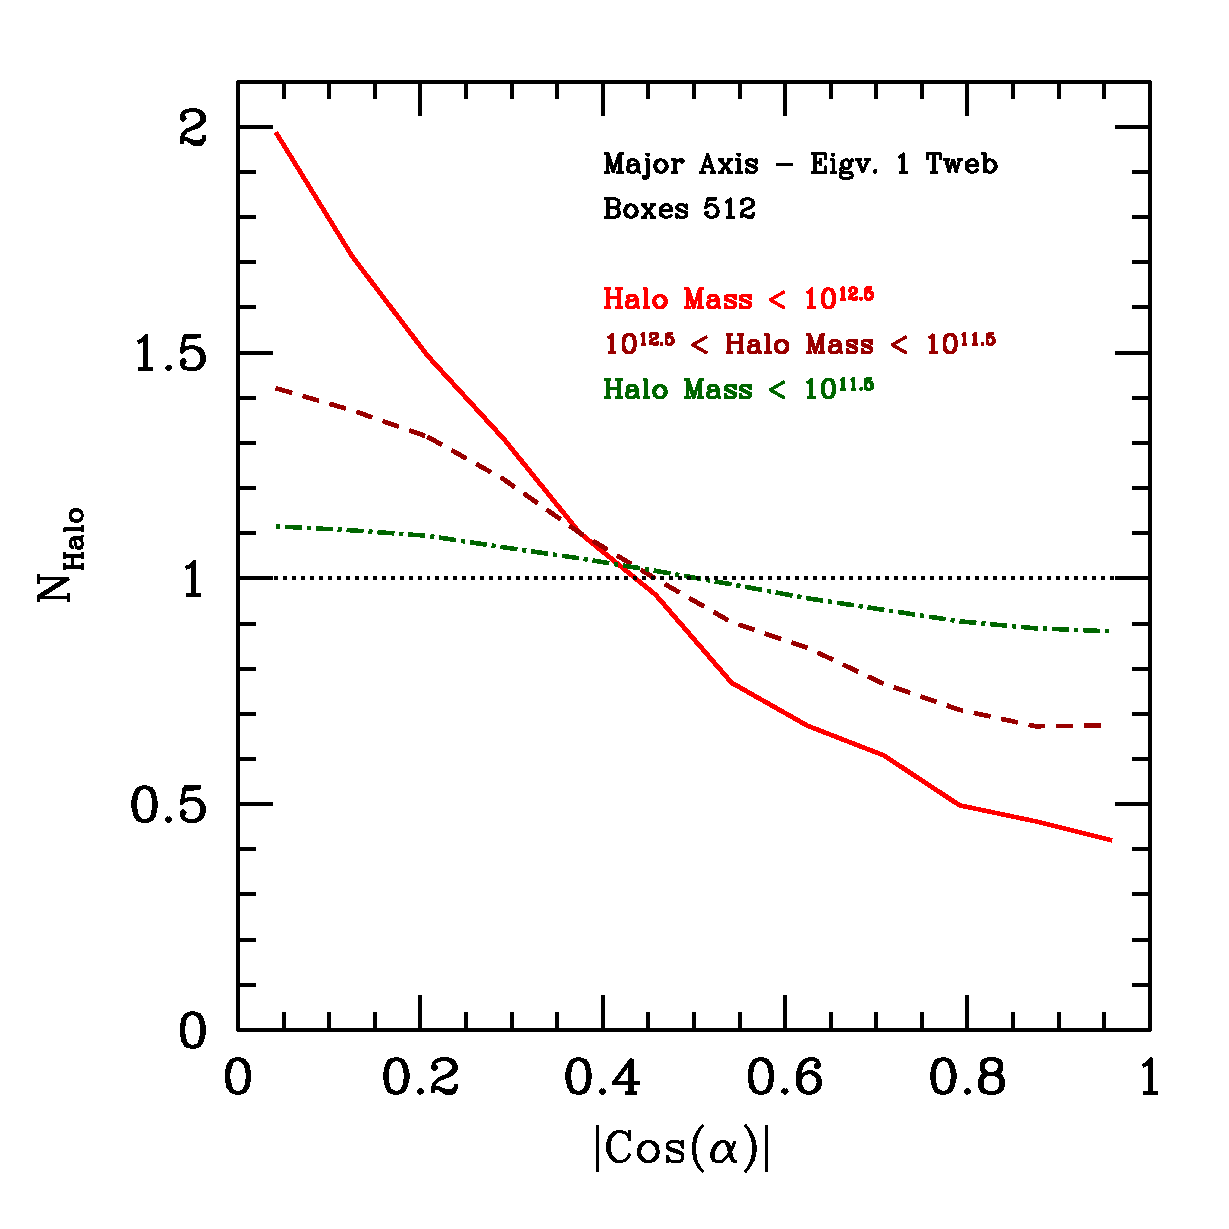
\includegraphics[width=0.30\textwidth]{../plot2/Ax1_VT/512_AX1_T1.ps}
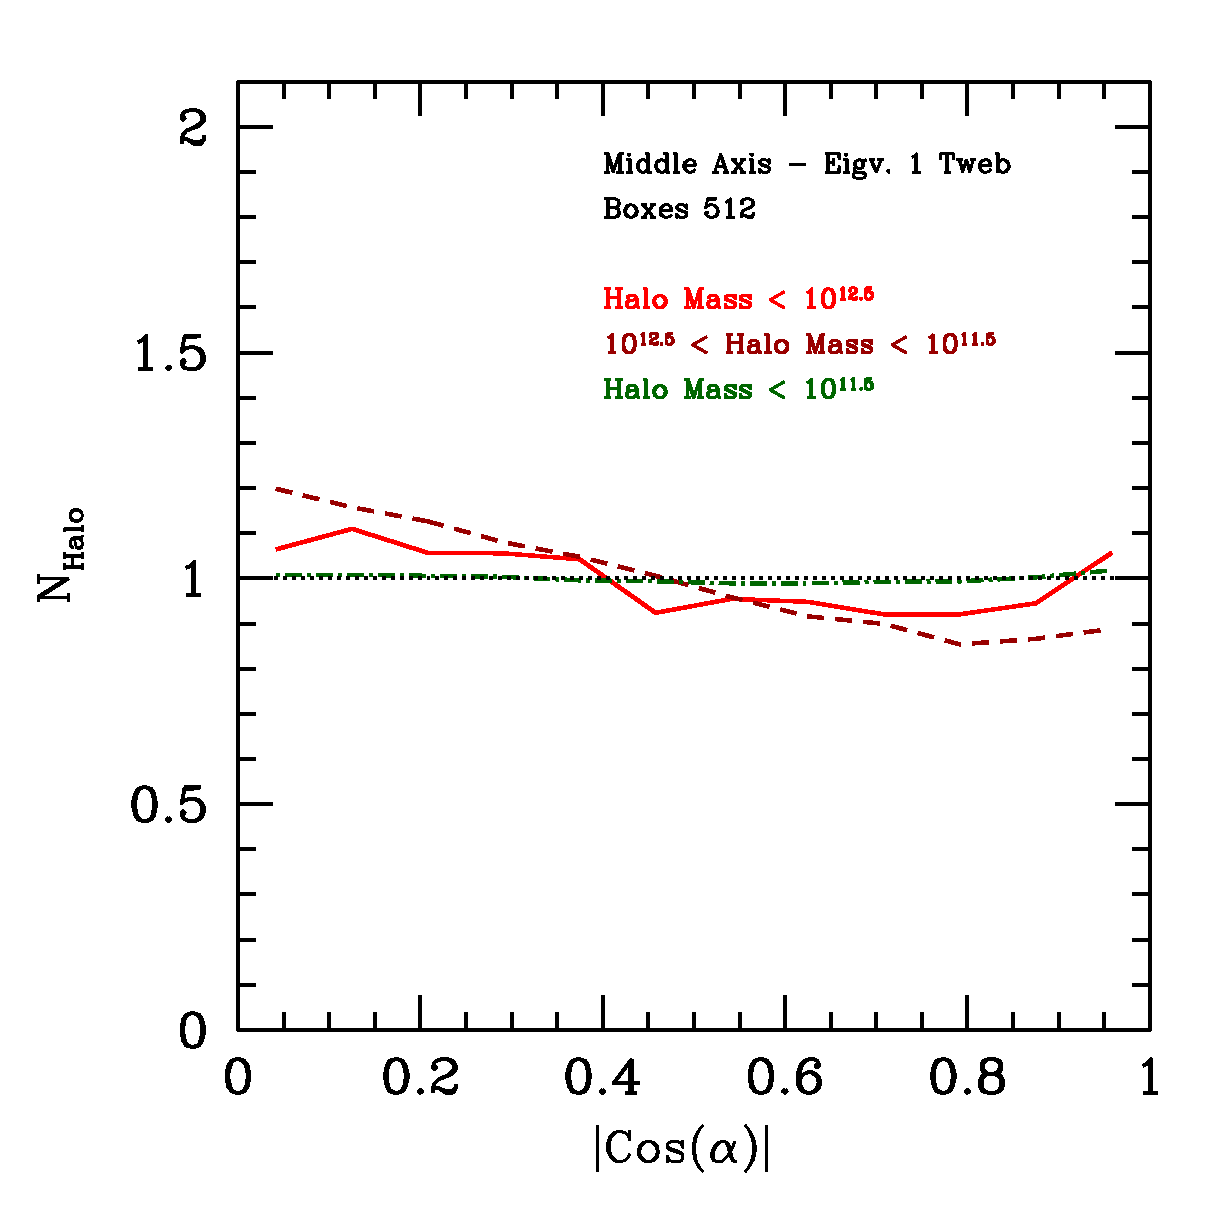
\includegraphics[width=0.30\textwidth]{../plot2/Ax2_VT/512_AX2_T1.ps}
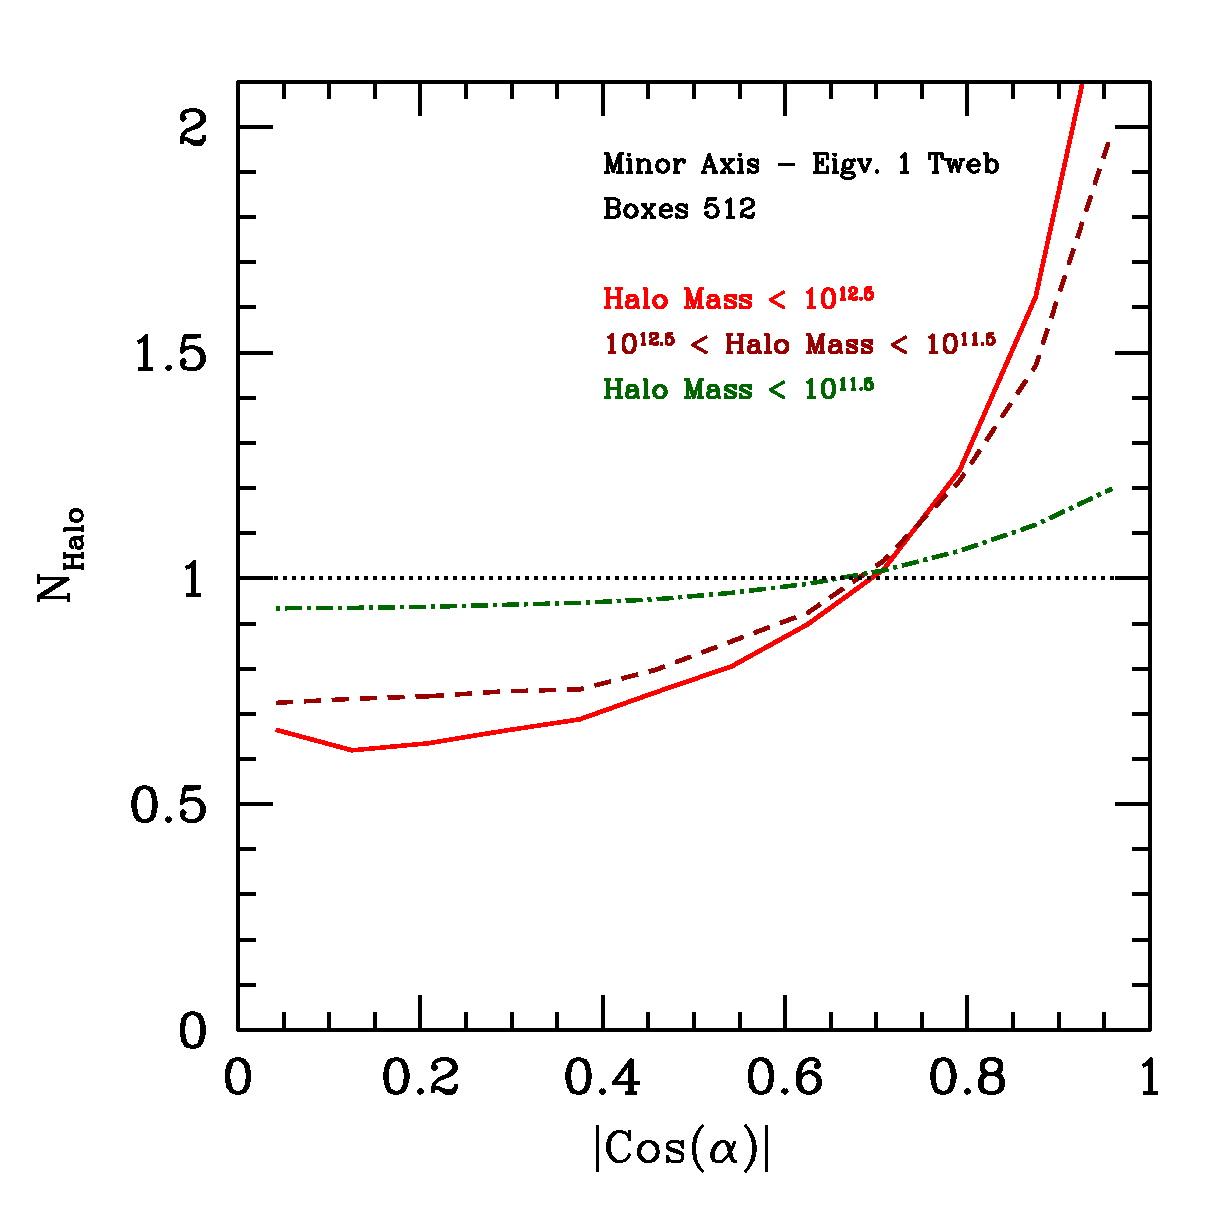
\includegraphics[width=0.30\textwidth]{../plot2/Ax3_VT/512_AX3_T1.ps}
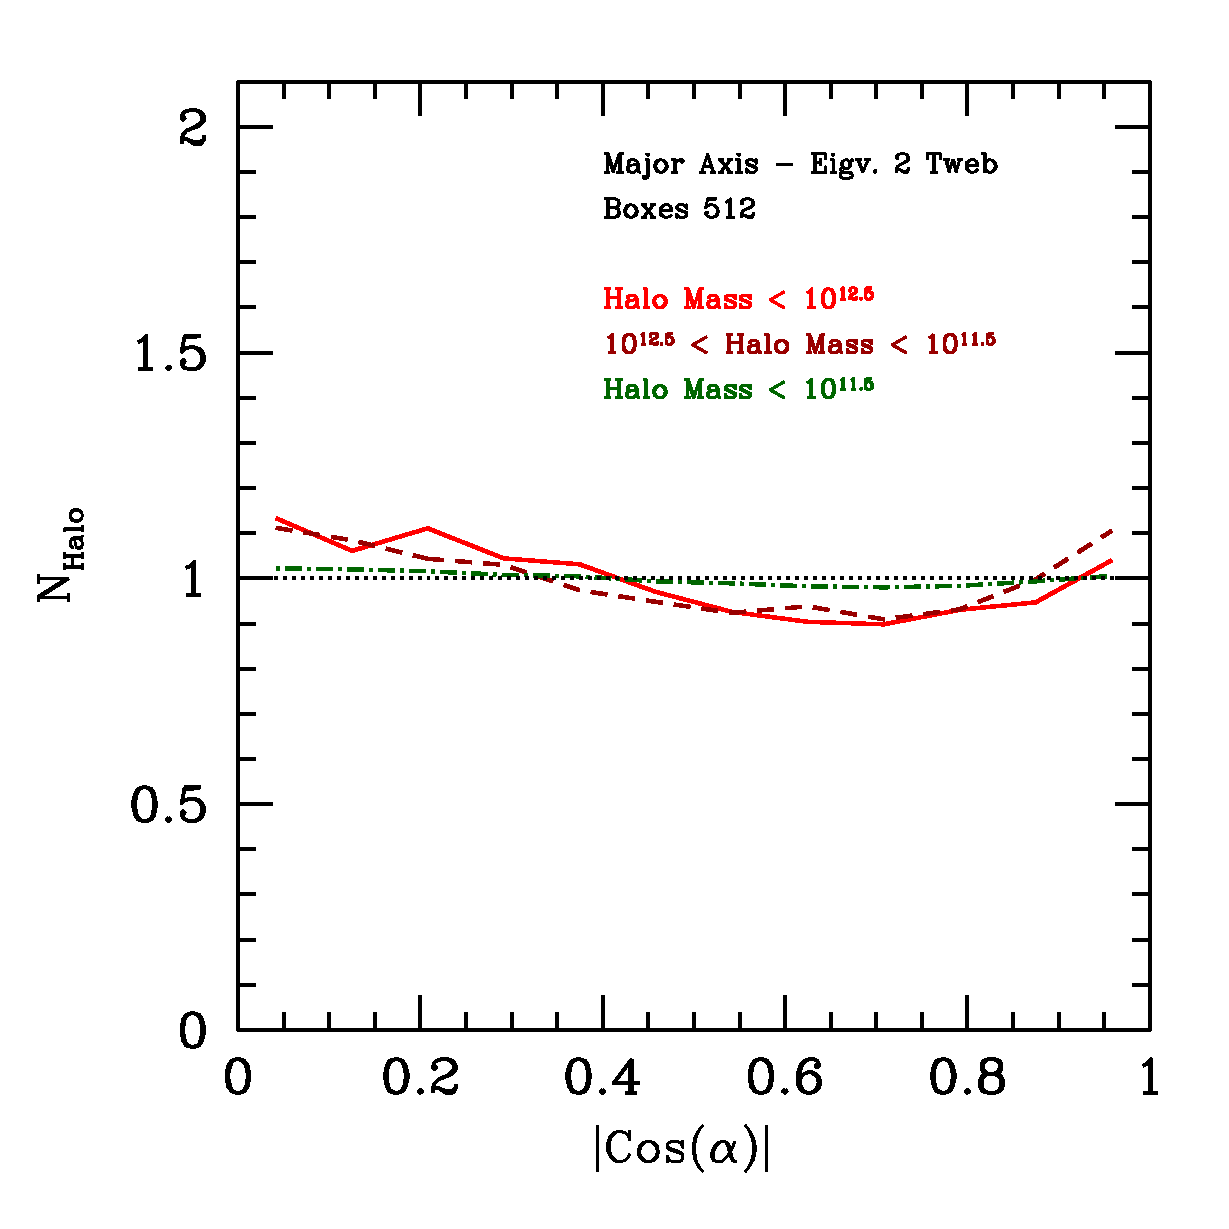
\includegraphics[width=0.30\textwidth]{../plot2/Ax1_VT/512_AX1_T2.ps}
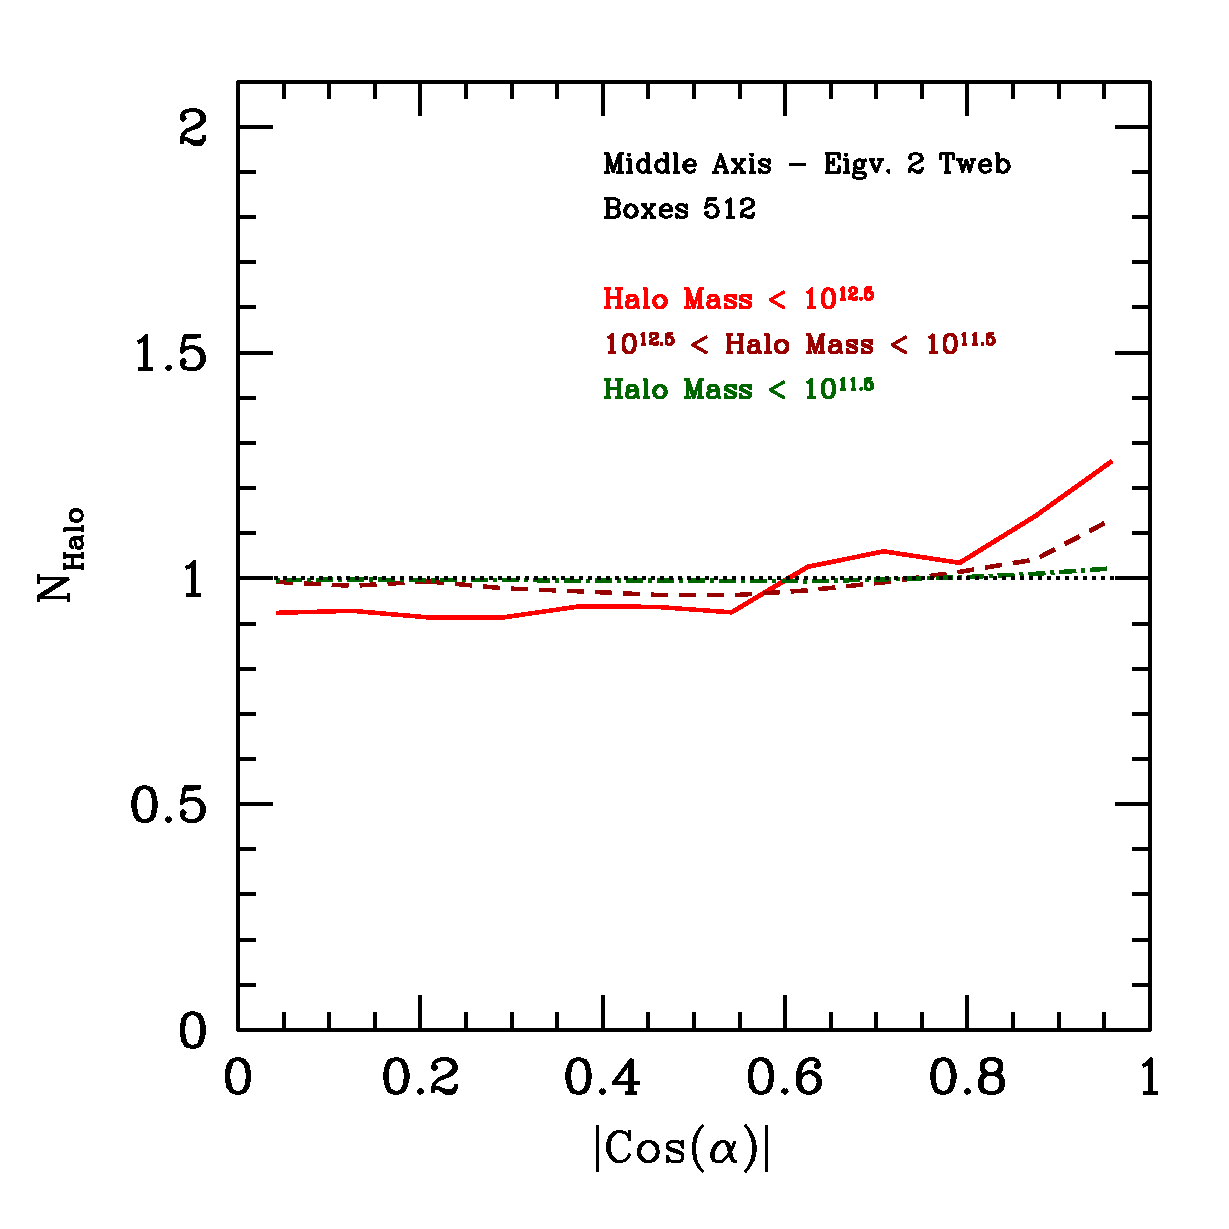
\includegraphics[width=0.30\textwidth]{../plot2/Ax2_VT/512_AX2_T2.ps}
\includegraphics[width=0.30\textwidth]{../plot2/Ax3_VT/512_AX3_T2.ps}
\includegraphics[width=0.30\textwidth]{../plot2/Ax1_VT/512_AX1_T3.ps}
\includegraphics[width=0.30\textwidth]{../plot2/Ax2_VT/512_AX2_T2.ps}
\includegraphics[width=0.30\textwidth]{../plot2/Ax3_VT/512_AX3_T3.ps}
\caption{Shape alignment for the tweb at $512^3$ resolution.}
\end{figure*}




\newpage
\subsection{Angular Momentum Alignment}

\begin{figure*}
\includegraphics[width=0.30\textwidth]{../plot2/J/256_J_V1.ps}
\includegraphics[width=0.30\textwidth]{../plot2/J/256_J_V2.ps}
\includegraphics[width=0.30\textwidth]{../plot2/J/256_J_V3.ps}
\caption{Angular momentum alignment with the Vweb for $256^3$ grid resolution.}
\end{figure*}


\begin{figure*}
\includegraphics[width=0.30\textwidth]{../plot2/J/512_J_V1.ps}
\includegraphics[width=0.30\textwidth]{../plot2/J/512_J_V2.ps}
\includegraphics[width=0.30\textwidth]{../plot2/J/512_J_V3.ps}
\caption{Angular momentum alignment with the Vweb for $512^3$ grid resolution.}
\end{figure*}


\begin{figure*}
\includegraphics[width=0.30\textwidth]{../plot2/J/256_J_T1.ps}
\includegraphics[width=0.30\textwidth]{../plot2/J/256_J_T2.ps}
\includegraphics[width=0.30\textwidth]{../plot2/J/256_J_T3.ps}
\caption{Angular momentum alignment with the Tweb for $256^3$ grid resolution.}
\end{figure*}


\begin{figure*}
\includegraphics[width=0.30\textwidth]{../plot2/J/512_J_T1.ps}
\includegraphics[width=0.30\textwidth]{../plot2/J/512_J_T2.ps}
\includegraphics[width=0.30\textwidth]{../plot2/J/512_J_T3.ps}
\caption{Angular momentum alignment with the Tweb for $512^3$ grid resolution.}
\end{figure*}



\subsection{Peculiar velocity Alignment}

\begin{figure*}
\includegraphics[width=0.30\textwidth]{../plot2/Vel/256_vel_V1.ps}
\includegraphics[width=0.30\textwidth]{../plot2/Vel/256_vel_V2.ps}
\includegraphics[width=0.30\textwidth]{../plot2/Vel/256_vel_V3.ps}
\caption{Peculiar velocity alignment with the Vweb for $256^3$ grid resolution.}
\end{figure*}


\begin{figure*}
\includegraphics[width=0.30\textwidth]{../plot2/Vel/512_vel_V1.ps}
\includegraphics[width=0.30\textwidth]{../plot2/Vel/512_vel_V2.ps}
\includegraphics[width=0.30\textwidth]{../plot2/Vel/512_vel_V3.ps}
\caption{Peculiar velocity alignment with the Vweb for $512^3$ grid resolution.}
\end{figure*}


\begin{figure*}
\includegraphics[width=0.30\textwidth]{../plot2/Vel/256_vel_T1.ps}
\includegraphics[width=0.30\textwidth]{../plot2/Vel/256_vel_T2.ps}
\includegraphics[width=0.30\textwidth]{../plot2/Vel/256_vel_T3.ps}
\caption{Peculiar velocity alignment with the Tweb for $256^3$ grid resolution.}
\end{figure*}


\begin{figure*}
\includegraphics[width=0.30\textwidth]{../plot2/Vel/512_vel_T1.ps}
\includegraphics[width=0.30\textwidth]{../plot2/Vel/512_vel_T2.ps}
\includegraphics[width=0.30\textwidth]{../plot2/Vel/512_vel_T3.ps}
\caption{Peculiar velocity alignment with the Tweb for $512^3$ grid resolution.}
\end{figure*}



\section{Discussion}
\label{sec:discussion}


\section{Conclusions}
\label{sec:conclusions}


\section*{Acknowledgments} 

\bibliographystyle{mn2e}
\bibliography{references} 



\end{document}
